%  A simple AAU PhD thesis template (collection of papers).
%  2016-08-01 v. 1.3.1
%  Copyright 2012-2016 by Jesper Kjær Nielsen <jkn@es.aau.dk>
%
%  This is free software: you can redistribute it and/or modrighte{caption}
\captionsetup{%
  font=footnotesize,% set font size to footnotesize
  labelfont=bf % bold label (e.g., Figure 3.2) font
}
% Make the standard latex tables look so much better
\usepackage{array,booktabs}
\usepackage{tabularx}
\usepackage{multirow}
% Enable the use of frames around, e.g., theorems
% The framed package is used in the example environment
\usepackage{framed}
% Create beautiful plots using TikZ and PGFPLOTS
\usepackage{tikz,pgfplots}
%%%%%%%%%%%%%%%%%%%%%%%%%%%%%%%%%%%%%%%%%%%%%%%%
% Mathematics
% http://en.wikibooks.org/wiki/LaTeX/Mathematics
%%%%%%%%%%%%%%%%%%%%%%%%%%%%%%%%%%%%%%%%%%%%%%%%
% Defines new environments such as equation,
% align and split 
\usepackage{amsmath}
% Adds new math symbols
\usepackage{amssymb}
\usepackage{mathtools}

% Use theorems in your document
% The ntheorem package is also used for the example environment
% When using thmmarks, amsmath must be an option as well. Otherwise \eqref doesn't work anymore.
\usepackage[framed,amsmath,amsthm,thmmarks]{ntheorem}

%%%%%%%%%%%%%%%%%%%%%%%%%%%%%%%%%%%%%%%%%%%%%%%%
% Page Layout and appearance
% http://en.wikibooks.org/wiki/LaTeX/Page_Layout
%%%%%%%%%%%%%%%%%%%%%%%%%%%%%%%%%%%%%%%%%%%%%%%%
% Change margins, papersize, etc of the document
\usepackage[
  paperwidth=17cm, % width of a page
  paperheight=24cm, % height of a page
  outer=2.5cm, % right margin on an odd page
  inner=2.5cm, % left margin on an odd page
  top=2.5cm, % top margin
  bottom=2.5cm % bottom margin
  ]{geometry}
% Enable the crop package if you want to print on a4 paer
%\usepackage[a4,cam,center]{crop}
% Modify how \chapter, \section, etc. look
% \renewcommand{\thesection}{\arabic{section}}
% The titlesec package is very configureable
\usepackage{titlesec}
\titleformat*{\section}{\normalfont\Large\bfseries\color{aaublue}}
\titleformat*{\subsection}{\normalfont\large\bfseries\color{aaublue}}
\titleformat*{\subsubsection}{\normalfont\normalsize\bfseries\color{aaublue}}
%\titleformat*{\paragraph}{\normalfont\normalsize\bfseries\color{aaublue}}
%\titleformat*{\subparagraph}{\normalfont\normalsize\bfseries\color{aaublue}}
% Change some default names
\addto\captionsenglish{%this line is required when using the babel package
  % \renewcommand\appendixname{Paper} % change Appendix to Paper
  \renewcommand\bibname{References} % change Bibliography to references
  \renewcommand\figurename{Fig.} % change Figure to Fig.
}

% Change the headers and footers
\usepackage{fancyhdr}
\pagestyle{fancy}
\fancyhf{} %delete everything
\renewcommand{\headrulewidth}{0pt} %remove the horizontal line in the header
\fancyhead[CE]{\color{aaublue}\small\nouppercase\leftmark} %even page - chapter title
\fancyhead[CO]{\color{aaublue}\small\nouppercase\rightmark} %uneven page - section title
\fancyfoot[CE,CO]{\thepage} %page number on all pages
% Do not stretch the content of a page. Instead,
% insert white space at the bottom of the page
\raggedbottom
% Enable arithmetics with length. Useful when
% typesetting the layout.
\usepackage{calc}
% fix the marginpar command so it is always on the correct side
\usepackage{mparhack}


\usepackage{longtable}

%%%%%%%%%%%%%%%%%%%%%%%%%%%%%%%%%%%%%%%%%%%%%%%%
% Bibliography
% http://en.wikibooks.org/wiki/LaTeX/Bibliography_Management
%%%%%%%%%%%%%%%%%%%%%%%%%%%%%%%%%%%%%%%%%%%%%%%%
% Bibliography for each chapter
% \usepackage[sectionbib]{chapterbib}
% Custom bibliograhy - used in the list of papers
\usepackage[resetlabels]{multibib}
% \usepackage[style=ieee, backend=biber]{biblatex}
% \addbibresource{bib/mybib.bib}

\newcites{main}{References}
\newcites{A}{Main Publications}
\newcites{B}{Publications with a Supervisory Role}
\newcites{C}{Miscellaneous Publications}
% \renewcommand*{\bibliographyitemlabel}{[\alph{enumiv}]}

% \makeatletter
% \newrobustcmd*{\mknumAlph}[1]{%
%   \begingroup
%   \blx@tempcnta=#1\relax
%   \ifnum\blx@tempcnta>702 %
%   \else
%     \ifnum\blx@tempcnta>26 %
%       \advance\blx@tempcnta\m@ne
%       \divide\blx@tempcnta26\relax
%       \blx@numalph\blx@tempcnta
%       \multiply\blx@tempcnta26\relax
%       \blx@tempcnta=\numexpr#1-\blx@tempcnta\relax
%     \fi
%   \fi
%   \blx@numAlph\blx@tempcnta
%   \endgroup}
% \def\blx@numAlph#1{%
%   \ifcase#1\relax\blx@warning@entry{Value out of range}\number#1\or
%   A\or B\or C\or D\or E\or F\or G\or H\or I\or J\or K\or L\or M\or
%   N\or O\or P\or Q\or R\or S\or T\or U\or V\or W\or X\or Y\or Z\else
%   \blx@warning@entry{Value out of range}\number#1\fi}
% \makeatother

% \DeclareFieldFormat{labelnumber}{\ifkeyword{mine}{\mknumAlph{#1}}{#1}}



% Change [1,2,3,4] into [1-4]
% \usepackage{cite}

%%%%%%%%%%%%%%%%%%%%%%%%%%%%%%%%%%%%%%%%%%%%%%%%
% Misc
%%%%%%%%%%%%%%%%%%%%%%%%%%%%%%%%%%%%%%%%%%%%%%%%
% Add bibliography and index to the table of
% contents
\usepackage{tocbibind}
% Enable subappendices
\usepackage{appendix}
\renewcommand{\setthesection}{\Alph{section}} % remove the chapter numbering
% Add the command \pageref{LastPage} which refers to the
% page number of the last page
\usepackage{lastpage}
% Add notes to in your document
\usepackage[
%  disable, %turn off todonotes
  colorinlistoftodos, %enable a coloured square in the list of todos
  textwidth=2cm, %set the width of the todonotes
  textsize=scriptsize, %size of the text in the todonotes
  ]{todonotes}
\setlength{\marginparwidth}{2cm}

%%%%%%%%%%%%%%%%%%%%%%%%%%%%%%%%%%%%%%%%%%%%%%%%
% Hyperlinks
% http://en.wikibooks.org/wiki/LaTeX/Hyperlinks
%%%%%%%%%%%%%%%%%%%%%%%%%%%%%%%%%%%%%%%%%%%%%%%%
% Enable hyperlinks and insert info into the pdf
% file. Hypperref should be loaded as one of the 
% last packages
\usepackage{hyperref}
\hypersetup{%
	pdfpagelabels=true,%
	plainpages=false,%
	pdfauthor={Author},%
	pdftitle={Title},%
	pdfsubject={Subject},%
	bookmarksnumbered=true,%
	colorlinks=true,%
	citecolor=aaublue,%
	filecolor=aaublue,%
	linkcolor=aaublue,% you should probably change this to black before printing
	urlcolor=aaublue,%
	pdfstartview=FitH%
}

\usepackage{xcolor}
\def\SBcomment[#1]{\textcolor{Red}{#1}}
\def\SWcomment[#1]{\textcolor{Cyan}{#1}}
\def\MDcomment[#1]{\textcolor{Green}{#1}}
\def\SScomment[#1]{\textcolor{Bittersweet}{#1}}

\usepackage{cases}
\usepackage[final]{pdfpages}

\usepackage{dirtytalk}
\usepackage{subfig}

\usepackage{tikz}
\tikzset{>=latex}
\tikzstyle{block} = [draw,minimum size=0.5cm]
\usetikzlibrary{math,arrows,positioning,shapes.geometric, decorations.markings}

\usepackage{listings}
\usepackage{courier}

\usepackage[most]{tcolorbox}
\usepackage{tabstackengine}
\stackMath


\def\eqrefMatlab[#1]{%
    \hypersetup{linkcolor=[HTML]008400}%
    \color[HTML]{008400}{\texttt{(\ref{#1}})}
}

\renewcommand{\lstlistingname}{Algorithm}% 
\def\setlstCpp
{
  \lstset{ %
  backgroundcolor=\color{black!0},   % choose the background color; you must add \usepackage{color} or \usepackage{xcolor}
  basicstyle=\footnotesize\ttfamily,        % the size of the fonts that are used for the code
  breakatwhitespace=true,         % sets if automatic breaks should only happen at whitespace
  breaklines=true,                 % sets automatic line breaking
  captionpos=b,                    % sets the caption-position to bottom
  commentstyle=\color[HTML]{008400},    % comment style
  % escapeinside={\%*}{*)},          % if you want to add LaTeX within your code
  extendedchars=true,              % lets you use non-ASCII characters; for 8-bits encodings only, does not work with UTF-8
  frame=tb,	                   	   % adds a frame around the code
  keepspaces=true,                 % keeps spaces in text, useful for keeping indentation of code (possibly needs columns=flexible)
  keywordstyle=\color[HTML]{B82BA1},       % keyword style
  language=C++,                 % the language of the code (can be overrided per snippet)
  % otherkeywords={*,...},           % if you want to add more keywords to the set
  numbers=none,                    % where to put the line-numbers; possible values are (none, left, right)
  numbersep=5pt,                   % how far the line-numbers are from the code
  numberstyle=\tiny\color{black},%\noncopynumber, % the style that is used for the line-numbers
  rulecolor=\color{black},         % if not set, the frame-color may be changed on line-breaks within not-black text (e.g. comments (green here))
  showspaces=false,                % show spaces everywhere adding particular underscores; it overrides 'showstringspaces'
  showstringspaces=false,          % underline spaces within strings only
  showtabs=false,                  % show tabs within strings adding particular underscores
  stepnumber=1,                    % the step between two line-numbers. If it's 1, each line will be numbered
  stringstyle=\color[HTML]{D12F1B}, % string literal style
  tabsize=2,	                   % sets default tabsize to 2 spaces
  title=\lstname,                  % show the filename of files included with \lstinputlisting; also try caption instead of title
  columns=fixed,                    % Using fixed column width (for e.g. nice alignment),
  deletekeywords={*, float},            % if you want to delete keywords from the given language
  }
}

\def\setlstMAT
{
  \lstset{ %
    backgroundcolor=\color[HTML]{FCFDDB},   % choose the background color; you must add \usepackage{color} or \usepackage{xcolor}
    basicstyle=\footnotesize\ttfamily,        % the size of the fonts that are used for the code
    breakatwhitespace=false,         % sets if automatic breaks should only happen at whitespace
    breaklines=true,                 % sets automatic line breaking
    captionpos=b,                    % sets the caption-position to bottom
    commentstyle=\color[HTML]{008400},    % comment style
    escapeinside={\%*}{*)},          % if you want to add LaTeX within your code
    extendedchars=true,              % lets you use non-ASCII characters; for 8-bits encodings only, does not work with UTF-8
    frame=tb,	                   	   % adds a frame around the code
    keepspaces=true,                 % keeps spaces in text, useful for keeping indentation of code (possibly needs columns=flexible)
    keywordstyle=\color[HTML]{0000FF},       % keyword style
    language=MATLAB,                 % the language of the code (can be overrided per snippet)
    otherkeywords={...},           % if you want to add more keywords to the set
    numbers=left,                    % where to put the line-numbers; possible values are (none, left, right)
    numbersep=5pt,                   % how far the line-numbers are from the code
    numberstyle=\tiny\color{black},%\noncopynumber, % the style that is used for the line-numbers
    rulecolor=\color{black},         % if not set, the frame-color may be changed on line-breaks within not-black text (e.g. comments (green here))
    showspaces=false,                % show spaces everywhere adding particular underscores; it overrides 'showstringspaces'
    showstringspaces=false,          % underline spaces within strings only
    showtabs=false,                  % show tabs within strings adding particular underscores
    stepnumber=1,                    % the step between two line-numbers. If it's 1, each line will be numbered
    stringstyle=\color[HTML]{A100F4}, % string literal style
    tabsize=2,	                   % sets default tabsize to 2 spaces
    title=\lstname,                  % show the filename of files included with \lstinputlisting; also try caption instead of title
    columns=fixed,                   % Using fixed column width (for e.g. nice alignment)
    deletekeywords={pi, zeros, plot, round, ceil, floor, cos, sin},            % if you want to delete keywords from the given language
    morestring=[b]"
  }
}

% package inclusion and set up of the document
\input{setup/hyphenations.tex}% 
\input{setup/macros.tex}% my new macros

\begin{document}
\DeclareGraphicsExtensions{.png,.jpg,.pdf, eps.}

% \def\bLabel{\renewcommand\@biblabel[1]{[##1]}}
% \def\citeP[#1]{[\hyperref[ch:listOfPublications]{#1}]}
\def\citeP[#1]{[\ref{paper:#1}]}

\def\ctxt{\text{c}} %connection subscript (text)
\def\stxt{\text{s}} %string subscript (text)
\def\ptxt{\text{p}} %plate subscript (text)
\def\mtxt{\text{m}} %mass subscript (text)
\def\itxt{\text{i}} %point of 'interest' subscript (text)
\def\Btxt{\text{B}} %bow subscript (text)
\def\etxt{\text{e}} %excitation subscript (text)
\def\rtxt{\text{r}} %lip reed subscript (text)
\def\ttxt{\text{t}} %tube subscript (text)

\def\sgn{\text{sgn}}
\def\sm{\text{sm}} %string-mass interaction tromba
\def\mp{\text{mp}} %mass-plate interaction tromba

\def\Nfrac{\mathcal{N}}
\def\flip{\leftarrow}
\def\Ucal{\mathbfcal{U}}

% states
\def\uln{u_l^n}
\def\wln{w_l^n}
\def\wmn{w_m^n}
\def\un{u^n}
\def\ulmn{u_{l,m}^n}
\def\ulm{u_{l,m}}
\def\uqn{u_q^n}

\def\wlmn{w_{l,m}^n}
\def\zlmn{z_{l,m}^n}
\def\ubr{u_\text{br}}
\def\zbr{z_\text{br}}

\def\qln{q_l^n}
\def\ulun{u_{l_u}^n}
\def\ulcn{u_{l_\ctxt}^n}
\def\wlwn{w_{l_w}^n}
\def\wmcn{w_{m_\ctxt}^n}

\def\wmn{w_m^n}

\def\Psiln{\Psi_l^n}
\def\Psinp{\Psi_l^{n+1}}
\def\Psinm{\Psi_l^{n-1}}
\def\Psilp{\Psi_{l+1}^n}
\def\Psilm{\Psi_{l-1}^n}

% bold symbols (state vectors and matrices)
\def\u{\mathbf{u}}
\def\w{\mathbf{w}}
\def\I{\mathbf{I}}
\def\A{\mathbf{A}}
\def\B{\mathbf{B}}
\def\C{\mathbf{C}}
\def\Q{\mathbf{Q}}
\def\U{\mathbf{U}}
\def\J{\mathbf{J}}
\def\i{\mathbf{i}}
\def\j{\mathbf{j}}

% interpolators
\def\Iu{I_{l, u}(x_\ctxt)}
\def\Iw{I_{m, w}(\chi_\ctxt)}
\def\Ju{J_{l, u}(x_\ctxt)}
\def\Jw{J_{m, w}(\chi_\ctxt)}
\def\Iq{I_q(\chi_\ctxt)}
\def\Ilm{I_{l,m}(x_\ctxt)}

\def\uStack{\boldsymbol{u}}
% mathfraks
\def\H{\mathfrak{H}}
\def\h{\mathfrak{h}}
\def\t{\mathfrak{t}}
\def\v{\mathfrak{v}}
\def\q{\mathfrak{q}}
\def\b{\mathfrak{b}}
\def\p{\mathfrak{p}}
% continuous operators
\def\ptt{\partial_t^2} 
\def\pxx{\partial_x^2}
\def\pxxx{\partial_x^3}
\def\pxxxx{\partial_x^4}

\def\pyy{\partial_y^2}

\def\pt{\partial_t} 
\def\px{\partial_x} 
\def\py{\partial_y} 

% discrete operators
\def\dtt{\delta_{tt}} 
\def\dxx{\delta_{xx}}
\def\dxxx{\delta_{xxx}}
\def\dxxxx{\delta_{xxxx}}
\def\dcc{\delta_{\chi\chi}}
\def\dcccc{\delta_{\chi\chi\chi\chi}}

\def\dtd{\delta_{t\cdot}} 
\def\dtp{\delta_{t+}} 
\def\dtm{\delta_{t-}} 

\def\dxd{\delta_{x\cdot}} 
\def\dxp{\delta_{x+}} 
\def\dxm{\delta_{x-}} 
\def\dyd{\delta_{y\cdot}} 
\def\dyp{\delta_{y+}} 
\def\dym{\delta_{y-}} 

\def\mtt{\mu_{tt}} 
\def\mtd{\mu_{t\cdot}} 
\def\mtp{\mu_{t+}} 
\def\mtm{\mu_{t-}} 

\def\mxx{\mu_{xx}} 
\def\mxd{\mu_{x\cdot}} 
\def\mxp{\mu_{x+}} 
\def\mxm{\mu_{x-}} 

\def\dDelta{\delta_{\Delta}}
% \def\dDbox{\delta_{\Delta\boxplus}}
\def\dyy{\delta_{yy}}

% matrix operators
\def\Dxx{\mathbf{D}_{xx}}
\def\Dxxxx{\mathbf{D}_{xxxx}}
\def\DDeltamat{\mathbf{D}_\Delta}
\def\DDeltaDelta{\mathbf{D}_{\Delta\Delta}}

\def\Dyy{\mathbf{D}_{yy}}

% often-used variables
\def\sz{\sigma_{0}}
\def\so{\sigma_{1}}
\def\vrel{v_\text{rel}}
\def\Sbar{\bar{S}}
\def\Sm{S_{l-1/2}}
\def\Sp{S_{l+1/2}}

\def\szX[#1]{\sigma_{0,{#1}}}
\def\soX[#1]{\sigma_{1,{#1}}}

\def\fs{f_\text{s}}
\def\el{\epsilon_\text{l}}
\def\er{\epsilon_\text{r}}
% mathcals
\def\D{\mathcal{D}}
\def\L{\mathcal{L}}
\def\OO{\mathcal{O}}
\def\S{\mathcal{S}}

% flooring ceiling
\def\floor[#1]{\left\lfloor #1 \right\rfloor}
\def\ceil[#1]{\left\lceil #1 \right\rceil}
\def\ansatz{\ \overset{\mathcal{A}}{\Longrightarrow}\ }
% other
\def\qaq{\quad \text{and} \quad}
\def\qwiq{\quad \text{with} \quad}
\def\qwhq{\quad \text{where} \quad}

\def\mystrut{\rule[-.2\baselineskip]{0pt}{\baselineskip}}

\def\th{\textsuperscript{th} }
\def\thOrder{\textsuperscript{th}-order }

\def\boldPhi{\boldsymbol{\phi}}
\def\boldPsi{\boldsymbol{\Psi}}
\def\eig{\text{eig}}

%frontmatter
\frontmatter
\pagestyle{empty} %disable headers and footers
\pagenumbering{roman} %use roman page numbering in the frontmatter
\papertitlepage{%
Resurrecting the Tromba Marina: A Bowed Virtual Reality Instrument using Haptic Feedback and Accurate Physical Modelling}{paper:E}{%
  Silvin Willemsen, Razvan Paisa and Stefania Serafin
}{%
  The paper has been published in the\\
  \textit{Proceedings of the 17th Sound and Music Computing (SMC) Conference}, pp. 300--307, 2020.
}{%
  \copyright 2020 Silvin Willemsen et al. This is an open-access article distributed under the terms of the Creative Commons Attribution 3.0 Unported License, which permits unrestricted use, distribution, and reproduction in any medium, provided the original author and source are credited. The layout has been revised.
}
\thispagestyle{empty}
\noindent
\fontsize{9.5}{12}\selectfont % so that the department fits on the line
\begin{tabularx}{\textwidth}{@{}lX}
    Thesis submitted: & July 31, 2021\\
    \\
    PhD Supervisor: & Prof.\ Stefania Serafin\\
                    & Aalborg University\\
                    \\
    PhD Committee:  & Assoc. Prof. Olga Timcenko\\
                    & Aalborg University\\
                    \\
                    & Prof. Julius O. Smith \\
                    & Stanford University\\
                    \\
                    & Prof. Augusto Sarti\\
                    & Politecnico di Milano\\
                   \\
    PhD Series:    & Technical Faculty of IT and Design, Aalborg University\\
    \\
    Department: & Department of Architecture, Design and Media Technology
\end{tabularx}
\normalsize
\strut\vfill
\noindent
\begin{tabularx}{\textwidth}{@{}lX}
    ISSN: & xxxx-xxxx\\
    ISBN: & xxx-xx-xxxx-xxx-x\\
\end{tabularx}
\strut\vfill
\noindent Published by:\newline
Aalborg University Press\newline
Skjernvej 4A, 2nd floor\newline
DK – 9220 Aalborg Ø\newline
Phone: +45 99407140\newline
aauf@forlag.aau.dk\newline
forlag.aau.dk
\strut\vfill
\noindent \copyright{} Copyright: Silvin Willemsen\newline
\strut\vfill
\noindent Printed in Denmark by Rosendahls, 2021
\clearpage


% mainfile: ../master.tex
\chapter*{Author CV\markboth{Author CV}{Author CV}}\label{ch:cv}
\pagestyle{fancy}
% \addcontentsline{toc}{chapter}{Curriculum Vitae}
% \begin{tabularx}{\textwidth}{@{}Xr}
%     \Large Silvin Willemsen & \raisebox{-\totalheight/2}{\includegraphics[width=2cm]{frontmatter/cvPicture.png}}\\
% \end{tabularx}\par
% \vspace{0.5cm}\noindent
Silvin Willemsen received his BSc. in Industrial Design from Eindhoven  University of Technology in 2015 and his MSc. in Sound and Music Computing from Aalborg University in 2017. In 2018, he was appointed as a PhD Stipend at the Department of Architecture, Design and Media Technology at Aalborg University Copenhagen and was affiliated with the Multisensory Experience Lab. During the PhD project he supervised students following the Sound and Music Computing masters programme, and was involved with teaching the courses \textit{Physical Modelling for Sound Synthesis} and \textit{Sound Processing}.
% \chapter*{Acknowledgements\markboth{Acknowledgements}{Acknowledgements}}\label{ch:acknowledgements}
\pagestyle{fancy}
\addcontentsline{toc}{chapter}{Acknowledgements}

I would like to thank my mom..
% mainfile: ../master.tex
\chapter*{Abstract\markboth{Abstract}{Abstract}}\label{ch:Abstract}
\addcontentsline{toc}{chapter}{Abstract}
Over the past few decades, numerous strategies to virtualise traditional instruments have been developed. Although one could create digital musical instruments using pre-recorded samples of their real-life counterparts, the playability will not be captured. Instead, a simulation of the underlying physics of the instrument could be created, and is much more flexible to player interaction. This \textit{physical model} will allow a musician to be much more expressive when playing the digital instrument than if static samples were to be used. Using ad hoc hardware to control the simulation could potentially make the simulated instrument feel identical to the original.

% Physical models can be used to simulate traditional musical instruments that are too rare or valuable to be played. These cases 

% Furthermore, 
Applications of physical modelling for musical instruments include simulating instruments that are unplayable as they are too rare or vulnerable. A model of the underlying physics of the instrument could potentially resurrect the instrument making it available to the public again. 
Furthermore, as a simulation is not restricted by the laws of physics, one could extend the possibilities of the original instrument. Properties such as the material or geometry of an instrument could be dynamically changed which broadens the range of expression of the musician. One could even imagine physically impossible musical instruments which still exhibit a natural sound due to the underlying models.

In this project, finite-difference time-domain (FDTD) methods have been chosen, as they have an advantage in terms of generality and flexibility regarding the systems they can model. A drawback of these methods is that they are quite computationally expensive, and although many highly accurate models based on these methods have existed for years, the computing power to run them in real time has only recently become available. The main challenge %introduced by these methods 
% and physical modelling in general are: 
% \begin{enumerate}
%     \item the underlying physical model needs to be formulated, which gets increasingly complex for higher accuracy, and
%     \item  
is thus to run the simulations in real time to allow for proper player interaction.

This thesis presents the development and real-time implementation of various physical models of traditional musical instruments based on FDTD methods. These instruments include the trombone and more obscure instruments such as the hurdy gurdy and the tromba marina. Furthermore, a novel method is presented that paves the way for dynamic FDTD-based musical instrument simulations allowing for physically impossible instrument manipulations. Finally, this work doubles as an aid for beginners in the field of musical instrument simulations based on FDTD methods, and aims to provide a low-entry-level explanation of the literature and theory that the physical models are based on. 

\chapter*{Resum{\'e}\markboth{Resum{\'e}}{Resum{\'e}}}\label{ch:Resume}
\addcontentsline{toc}{chapter}{Resum{\'e}}
I l{\o}bet af de sidste {\aa}rtier, er der blevet udviklet adskillige strategier til at lave virtuelle udgaver af traditionelle musikinstrumenter. Selvom digitale musikinstrumenter baseret p{\aa} traditionelle musikinstrumenter, kan skabes ved hj{\ae}lp af lydoptagelser af deres virkelige modstykke, er det ofte p{\aa} bekostning instrumenternes spilbarhed.
En anden strategi ville v{\ae}re at implementere en digital simulering af instrumentets underliggende fysik, hvilket ville give en mere fleksibel og naturlig interaktion. Denne digitale simulering, en fysisk model af instrumentet, ville g{\o}re det muligt for en musiker at v{\ae}re mere udtryksfuld n{\aa}r han eller hun spiller p{\aa} det digitale musikinstrument end med statiske lydoptagelser. Derudover, ved at bruge ad hoc hardware til at styre simuleringen, kunne man potentielt f{\aa} det digitale musikinstrument til at f{\o}les identisk med originalen. 

Fysisk modellering af musikinstrumenter kan ogs{\aa} anvendes til at simulere musikinstrumenter, der er sj{\ae}ldne eller for s{\aa}rbare til at m{\aa} spilles p{\aa}. Her ville en model af instrumentets underliggende fysik potentielt kunne genoplive instrumentet ved g{\o}re det tilg{\ae}ngeligt og spilbart igen. Ydermere, kunne man forbedre det originale instrument, eftersom en digital simulering ikke er begr{\ae}nset af fysikkens love. Egenskaber som instruments materiale eller geometri kunne dynamisk {\ae}ndres og udvide musikerens udtryksmuligheder. Man kunne endda forestille sig fysisk umulige musikinstrumenter, der stadig har en naturlig klang p{\aa} grund af de underliggende modelleringsprincipper. 

Til dette projekt er finite-difference time-domain (FDTD) metoderne blevet valgt som modelleringsteknik, siden disse metoder er generelle og fleksible og derfor har en fordel i forhold til de forskellige typer af systemer som de kan modellere.  En ulempe ved FDTD metoderne er at de er beregningstunge, og selvom der har eksisteret n{\o}jagtige modeller baseret p{\aa} disse metoder i {\aa}revis, er computer regnekraften til at k{\o}re dem i realtid f{\o}rst blevet tilg{\ae}ngelig for nyligt. Den st{\o}rste udfordring er derfor at k{\o}re simuleringerne i realtid og at opn{\aa} naturlig interaktion imellem ud{\o}veren og simuleringen. 

Denne afhandling beskriver udviklingen og implementeringen af forskellige fysiske modeller af traditionelle musikinstrumenter baseret p{\aa} FDTD metoder i realtid. Disse instrumenter inkluderer trombone og mindre kendte instrumenter som drejelire og tromba marina. Desuden pr{\ae}senteres en ny metode, der muligg{\o}r dynamiske parametre i FDTD-baserede musikinstrumentsimuleringer og tillader instrumentmanipulationer som er umulige i den virkelige verden. 
Derudover, kan denne afhandling bruges som et hj{\ae}lpemiddel til begyndere inden for simuleringer af musikinstrumenter, og sigter mod at give en begyndervenlig forklaring af den litteratur og teori, som de fysiske modeller er baseret p{\aa}. 

% mainfile: ../master.tex
\chapter*{Preface\markboth{Preface}{Preface}}\label{ch:preface}
\pagestyle{fancy}
\addcontentsline{toc}{chapter}{Preface}

Starting this PhD, I did not have a background in mathematics, physics or computer science, which were three equally crucial components in creating the result of this project. This is why I decided to write this thesis a bit more pedagogical than what could be expected. As I felt that the literature lacks a lot of intuition I wanted to give that to the reader. Some basic calculus knowledge is assumed.  

I wanted to show my learning process and (hopefully) explain topics such as \textit{Energy Analysis}, \textit{Stability Analysis}, etc. in a way that others lacking the same knowledge %(/ with the same background) 
will be able to understand.

\textit{Interested in physically impossible manipulations of now-virtual instruments.}

\vfill
\hfill Silvin Willemsen

\hfill Aalborg University, \today

\chapter*{List of Publications\markboth{List of Publications}{List of Publications}}\label{ch:listOfPublications}
\pagestyle{fancy}
\addcontentsline{toc}{chapter}{List of Publications}
Listed below are the publications made during the PhD project, (co)authored by the PhD student. These are grouped by: the main publications, which are also included in Part \ref{part:papers}, papers with a supervisory role, and finally, other publications from various collaborative efforts.
{
 % make the scope for publications smaller
\makeatletter
\renewenvironment{thebibliography}[1]
     {\subsubsection*{\bibname}%
      \@mkboth{\MakeUppercase\bibname}{\MakeUppercase\bibname}%
      \list{\@biblabel{\@Alph\c@enumiv}}%
           {\settowidth\labelwidth{\@biblabel{\@Alph#1}}%
            \leftmargin\labelwidth
            \advance\leftmargin\labelsep
            \@openbib@code
            \usecounter{enumiv}%
            \let\p@enumiv\@empty
            \renewcommand\theenumiv{\@Alph\c@enumiv}}%
      \sloppy
      \clubpenalty4000
      \@clubpenalty \clubpenalty
      \widowpenalty4000%
      \sfcode`\.\@m}
     {\def\@noitemerr
       {\@latex@warning{Empty `thebibliography' environment}}%
      \endlist}
\makeatother

% removed the S-es here to unsort
\nociteM{*}
\bibliographystyleM{IEEEtran} 
\bibliographyM{bib/mainPapers}

\makeatletter
\renewenvironment{thebibliography}[1]
     {\subsubsection*{\bibname}%
      \@mkboth{\MakeUppercase\bibname}{\MakeUppercase\bibname}%
      \list{\@biblabel{S\@arabic\c@enumiv}}%
           {\settowidth\labelwidth{\@biblabel{S#1}}%
            \leftmargin\labelwidth
            \advance\leftmargin\labelsep
            \@openbib@code
            \usecounter{enumiv}%
            \let\p@enumiv\@empty
            \renewcommand\theenumiv{S\@arabic\c@enumiv}}%
      \sloppy
      \clubpenalty4000
      \@clubpenalty \clubpenalty
      \widowpenalty4000%
      \sfcode`\.\@m}
     {\def\@noitemerr
       {\@latex@warning{Empty `thebibliography' environment}}%
      \endlist}
\makeatother

\nociteS{*}
\bibliographystyleS{IEEEtran}
\bibliographyS{bib/supervisoryPapers}

\makeatletter
\renewenvironment{thebibliography}[1]
     {\subsubsection*{\bibname}%
      \@mkboth{\MakeUppercase\bibname}{\MakeUppercase\bibname}%
      \list{\@biblabel{O\@arabic\c@enumiv}}%
           {\settowidth\labelwidth{\@biblabel{M#1}}%
            \leftmargin\labelwidth
            \advance\leftmargin\labelsep
            \@openbib@code
            \usecounter{enumiv}%
            \let\p@enumiv\@empty
            \renewcommand\theenumiv{O\@arabic\c@enumiv}}%
      \sloppy
      \clubpenalty4000
      \@clubpenalty \clubpenalty
      \widowpenalty4000%
      \sfcode`\.\@m}
     {\def\@noitemerr
       {\@latex@warning{Empty `thebibliography' environment}}%
      \endlist}
\makeatother

\nociteO{*}
\bibliographystyleO{IEEEtran}
\bibliographyO{bib/otherPapers}

% \nociteA{*}
% {\bibliographystyleA{IEEEtranS}\bibliographyA{bib/mainPapers}}
% \nociteB{*}
% {\bibliographystyleB{IEEEtranS}\bibliographyB{bib/supervisoryPapers}}
% \nociteC{*}
% {\bibliographystyleC{IEEEtranS}\bibliographyC{bib/otherPapers}}

% \makeatletter
% \renewcommand\@bibitem[1]{\item\if@filesw \immediate\write\@auxout
%     {\string\bibcite{#1}{A\the\value{\@listctr}}}\fi\ignorespaces}% <------------
% \def\@biblabel#1{[A#1]}% <-------------------
% \makeatother
}
\chapter*{List of Symbols}\label{app:listOfSymbols}
The list of symbols found below contains often-used symbols in the thesis in the context that they are normally used. Depending on the context they might carry a different meaning ($y$ being displacement of the lip-reed in Chapter \ref{ch:trombone} but the vertical spatial coordinate for 2D systems in fx. Chapter \ref{ch:2Dsyst}). Some might also be accompanied by a subscript in the main document

{\centering\renewcommand{\arraystretch}{1.1}
\begin{longtable}{ p{2cm} p{6.5cm} p{2.5cm}  }
 Symbol & Description & Unit\\
 \hline\\
 \endhead
 $\alpha$ & Fractional part of & \\
 $A$ & Cross-sectional area of string & m$^2$\\
 $c$ & Wave speed & m/s\\
 $\frac{d^n}{dt^n}$ & $n$\textsuperscript{th} order derivative with respect to $t$ & - \\
 $\pt^n$ & $n$\textsuperscript{th} order partial derivative with respect to $t$ & - \\
 $\dtp$, $\dtm$, $\dtd$ & Forward, backward and centred difference in time operator & - \\
 $\dxp$, $\dxm$, $\dxd$ & Forward, backward and centred difference in space operator& - \\
 $\dtt$& Second order difference in time operator& - \\
 $\dxx$& Second order difference in space operator& - \\
 $\dxxxx$& Fourth order difference in space operator& - \\
 $\mtp$, $\mtm$, $\mtd$ & Forward, backward and centred average in time operator& - \\
 $\mxp$, $\mxm$, $\mxd$ & Forward, backward and centred average in space operator& - \\
 $\mtt$ & Second order average in time operator& -\\
 $\mxx$ & Second order average in space operator& -\\
 $E$ & Young's Modulus & Pa (kg$\cdot$m$^{-1}\cdot$s$^{-2}$)\\
 $f$ & Force & N\\
 $f$ & Frequency & Hz\\
 $f_\text{s}$ & Sample rate & Hz\\
 $h$ & Grid spacing & m \\ 
 $H$ & Membrane / Plate thickness & m \\ 
 $I$ & Area moment of inertia & m$^4$\\
 $l$ & Spatial index of a grid function & - \\
 $l,m$ & Spatial index of a 2D grid function & - \\
 $L$ & Length & m\\
 $L_x$ & Length in $x$-direction (2D) & m\\
 $L_y$ & Length in $y$-direction (2D) & m\\
 $k$ & Time step ($=1/f_\text{s}$) & s\\
 $K$ & Spring coefficient & N/m\\
 $\kappa$ & Stiffness coefficient & m$^2$/s \\
 $n$ & Sample index to grid function & - \\
 $N$ & Number of points string & -\\
 $N_x$ & Number of points $x$-direction (2D) & -\\
 $N_y$ & Number of points $y$-direction (2D) & -\\
 $\mathbb{N}^0$ & Set of non-negative integers %($\mathbb{N}^0 = 0, 1, 2, \hdots$) 
 & -\\
 $p$ & Pressure & Pa\\
 $r$ & Radius & m\\
 $S$ & Cross-sectional area (brass) & m$^2$\\
 $t$ & Time & s\\
 $T$ & Tension & N (1D)\\
 & & N/m (2D)\\
 $u$ & State variable & m\\ 
 $v$ & Particle velocity & m/s\\ 
 $x$ & Spatial dimension & m\\
 $y$ & Spatial dimension (2D) & m\\
 $\gamma$ & Scaled wave speed & s$^{-1}$\\
 $\lambda$ & Courant number for 1D wave eq. ($=ck/h$) & -\\
 $\mu$ & Stiffness \SWcomment[free parameter] & -\\
 $\nu$ & Poisson's ratio & -\\
 $\eta$ & Relative displacement & m\\
 $\rho$ & Material density & kg$\cdot$m$^{-3}$\\
 \\
    \hline {\bf Operations}\\\hline
 \\
 $\mathfrak{I}(\cdot)$ & Imaginary part of &\\
 $\mathfrak{R}(\cdot)$ & Real part of & \\
 $\floor[\cdot]$ & Flooring operation &\\
 $\ceil[\cdot]$ & Ceiling operation &\\
 \\\hline
 {\bf Subscripts}\\\hline
 \\
 $\ctxt$ & Connection &\\
 $\ptxt$ & Plate &\\
 $\stxt$ & String &
\end{longtable}}
\chapter{List of Abbreviations}
{\renewcommand{\arraystretch}{1.1}
\begin{tabular}{ p{3cm} p{7cm} p{4cm}  }
 Abbreviation & Definition\\
 \hline\\
 FDS & Finite-difference scheme\\
 FDTD & Finite-difference time-domain
\end{tabular}}

\cleardoublepage
\pdfbookmark[0]{Contents}{label:contents}
\pagestyle{fancy} %enable headers and footers again
\tableofcontents
% \listoffigures
% \listoftables 

\listoftodos
\cleardoublepage

\def\makeAlph[#1]{\symbol{\numexpr96+#1}}

%mainmatter
\mainmatter

\part{Introduction}\label{part:introduction}
\chapter*{Exciters}
Several resonators have been introduced in part \ref{part:resonators}, different mechanisms to excite them will be introduced here. First, different examples of 

and have a great effect on the eventual timbre of the sound. 
Chapter \ref{ch:physInspExcitations} presents various physically inspired excitations some of which made a brief appearance in Part \ref{part:resonators}. Chapter \ref{ch:bow} introduces a static and a dynamic friction model that can be used for bowing resonators. Additionally, this chapter presents the contribution made in \citeP[C]: the elasto-plastic friction model applied to FDTD stiff strings. Finally, Chapter \ref{ch:lipreed} presents the lip reed as a way to excite brass instruments. 


\part{Resonators}\label{part:resonators}
\chapter*{Exciters}
Several resonators have been introduced in part \ref{part:resonators}, different mechanisms to excite them will be introduced here. First, different examples of 

and have a great effect on the eventual timbre of the sound. 
Chapter \ref{ch:physInspExcitations} presents various physically inspired excitations some of which made a brief appearance in Part \ref{part:resonators}. Chapter \ref{ch:bow} introduces a static and a dynamic friction model that can be used for bowing resonators. Additionally, this chapter presents the contribution made in \citeP[C]: the elasto-plastic friction model applied to FDTD stiff strings. Finally, Chapter \ref{ch:lipreed} presents the lip reed as a way to excite brass instruments. 

\chapter{Stiff string}\label{ch:stiffString}
Earlier, the case of the ideal string was presented (Section \ref{sec:1DWave}) modelled using the 1D wave equation. As shown, the model generates an output with harmonic partials that are integer multiples of the fundamental frequency. In the real world, however, strings exhibit a phenomenon called \textit{inharmonicity} due to stiffness in the material. 

The restoring force of the 1D wave equation is only due to tension. In the real world, however, this force is also due to stiffness, dependent on the material and geometry of the string. This stiffness causes frequency dispersion and inharmonicity: the partials get exponentially further apart with frequency. 

The stiff string played a prominent part in many of the published works:
\citeP[A], \citeP[B], \citeP[C], \citeP[D] and \citeP[E]. 

This chapter 

\section{Continuous time}
Consider the transverse displacement of a lossless \todo{should I even include the lossless one? It's just so that we can slowly build up to the damped model...}stiff string of length $L$ described by $u=u(x,t)$ defined for $x\in \D$ with domain $\D = [0, L]$ and time $t\geq 0$. The PDE describing its motion is 
\begin{equation}\label{eq:stiffStringPDENoLosses}
    \rho A \ptt u = T \pxx u - EI \pxxxx u
\end{equation}
parameterised by material density $\rho$ (in kg/m$^3$), cross-sectional area $A = \pi r^2$ (in m$^2$), radius $r$ (in m) tension $T$ (in N), Young's modulus $E$ (in Pa) and area moment of inertia $I = \pi r^4/4$ (in m$^4$). If either $E$ or $I$ is 0, Eq \eqref{eq:stiffStringPDENoLosses} reduces to the 1D wave equation in \eqref{eq:1DwavePDE} where $c = \sqrt{T/\rho A}$. If instead $T = 0$, Eq. \eqref{eq:stiffStringPDENoLosses} reduces to the \textit{ideal bar} equation.


\subsubsection{Dispersion Analysis}
The 4th-order spatial derivative models \textit{frequency dispersion}, a phenomenon that causes different frequencies to travel at different speeds. As opposed to the undesired numerical dispersion 

\subsection{Adding Losses}
Before moving on to the discretisation of Eq. \eqref{eq:stiffStringPDENoLosses}, losses can be added to the system. This is done by simply adding terms to \eqref{eq:stiffStringPDENoLosses} according to \todo{First appeared in \cite{Bensa2003}}
\begin{equation}\label{eq:stiffStringPDE}
    \rho A \ptt u = T \pxx u - EI \pxxxx u - 2 \sz \rho A \pt u + 2 \so \rho A\pt \pxx u
\end{equation}
where the loss coefficients $\sz$ (in s$^{-1}$) and $\so$ (in m$^2$/s) describe the frequency dependent and frequency independent losses respectively. 

A more compact way to write Eq. \eqref{eq:stiffStringPDE}, and as is also found often in the literature \cite{theBible} \todo{etc.} is to divide both sides by $\rho A$ to get
\begin{equation}\label{eq:stiffStringPDECompact}
    \ptt u = c^2 \pxx u - \kappa^2 \pxxxx u - 2 \sz \pt u + 2 \so \pt \pxx u
\end{equation}
where $c=\sqrt{T/\rho A}$ is the wave speed \todo{check wavespeed or wave speed (entire document)} (in m/s) as in the 1D wave equation in \eqref{eq:1DwavePDE} and $\kappa = \sqrt{EI / \rho A}$ is a \textit{stiffness coefficient} (in m$^2$/s).

\subsubsection{Intuition}
Although Eq. \eqref{eq:stiffStringPDE} might look daunting at first, the principle of Newton's second law remains the same. 

Something about the 4th spatial derivative and the loss terms here...

\subsubsection{Boundary Conditions}
The boundary conditions found in Eq. \eqref{eq:boundaryCond1DWave} can be extended to
\begin{subequations}\label{eq:stiffStringBoundConds}
    \begin{align}
        u = \px u &= 0 \quad \text{(clamped)}\label{eq:BCclamped}\\
        u = \pxx u &= 0 \quad \text{(simply supported)}\label{eq:BCsimplySupported}\\
        \pxx u = \pxxx u &= 0 \quad \text{(free)}\label{eq:BCfree}
    \end{align}
\end{subequations}
at $x = 0, L$.
\todo{insert figure showing virtual grid points}

\section{Discrete Time}
For the sake of brevity, we continue with Eq. \eqref{eq:stiffStringPDECompact} (rather than Eq. \eqref{eq:stiffStringPDE}) which can be discretised as 
\begin{equation}\label{eq:stiffStringFDS}
    \dtt \uln = c^2 \dxx \uln - \kappa^2 \dxxxx \uln - 2 \sz \dtd \uln + 2 \so\dtm\dxx \uln,
\end{equation}
And domain $l\in\{0, \hdots, N\}$ and number of grid points $N+1$. The stability condition will be derived in Section \ref{sec:stiffStringStability} 

The $\dxxxx$ operator is the second-order spatial difference in Eq. \eqref{eq:discSecondSpace} applied to itself
\begin{equation}\label{eq:dxxxx}
    \dxxxx = \dxx\dxx = \frac{1}{h^4}\left(e_{x+}^2 - 4e_{x+}+6 - 4e_{x-}+e_{x-}^2\right).
\end{equation} \todo{explain the mixed operator here}

The reason a backwards difference is used here is to keep the system explicit. A centred operator could potentially be used, but then neighbouring points at the next time step, i.e., $u^{n+1}_{l+1}$ and $u^{n+1}_{l-1}$ would be needed to calculate $u^{n+1}_l$. 


Using 
\begin{equation}
    \lambda = \frac{ck}{h} \qaq \mu = \frac{\kappa k}{h^2},
\end{equation}
we can expand the operators and collect the terms to obtain the following update equation
\begin{equation}
    \begin{aligned}
    % (1+\sz k) u_l^{n+1} =&\ \left(2 - 2\lambda^2 - 6\mu^2 - \frac{4\so k}{h^2}\right) \uln\\
    % & + \left(\lambda^2 + 4\mu^2 + \frac{2\so k}{h^2}\right) (u_{l+1}^n + u_{l-1}^n) \\
    % &- \mu^2 (u_{l+2}^n + u_{l-2}^n) + \left(-1+\sz k + \frac{4\sz k}{h^2}\right)u_l^{n-1}\\
    % & - \frac{2\so k}{h^2}(u_{l+1}^{n-1} + u_{l-1}^{n-1})
    % \end{aligned}
    Au_l^{n+1} = &\ B_0 \uln + B_1 (u_{l+1}^n + u_{l-1}^n) + B_2 (u_{l+2}^n + u_{l-2}^n) \\
    &+ C_0 u_l^{n-1} + C_1(u_{l+1}^{n-1} + u_{l-1}^{n-1}) 
    \end{aligned}
\end{equation}
with coefficients
\begin{gather*}
    B_0 = 2 - 2\lambda^2 - 6\mu^2 - \frac{4\so k}{h^2}, \quad B_1 = \lambda^2 + 4\mu^2 + \frac{2\so k}{h^2}, \quad B_2 =- \mu^2, \\[1em]
    C_0 =  -1+\sz k + \frac{4\so k}{h^2},\quad C_1 = - \frac{2\so k}{h^2}, \qaq A = 1+\sz k.
\end{gather*}
Note that the division by $A$ has been left for implementation. 
\begin{figure}[h]
    \centering
    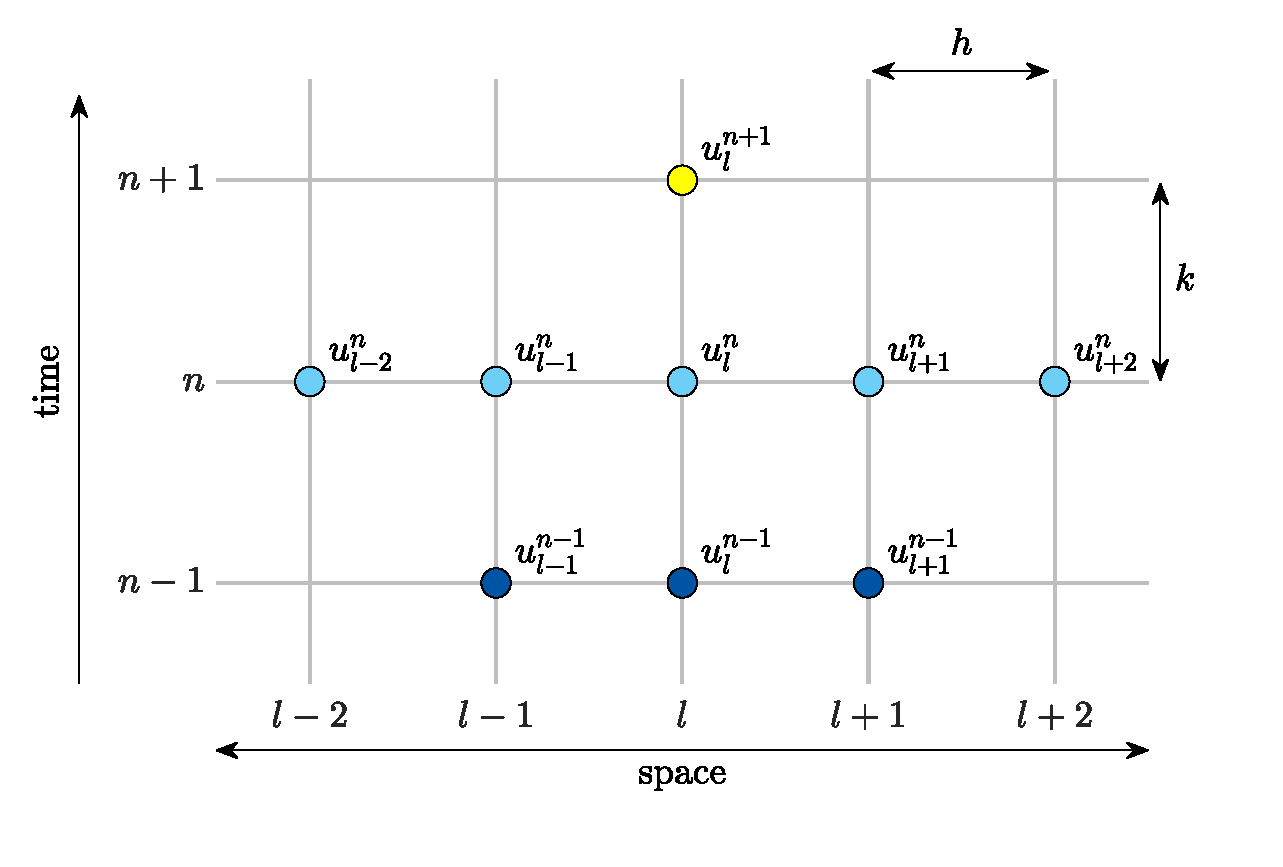
\includegraphics[width=0.8\textwidth]{figures/resonators/stencilDampedStiffString.eps}
    \caption{The stencil for the damped stiff string scheme in \eqref{eq:stiffStringFDS}.\label{fig:stencilStiffString}}
\end{figure}

\subsection{Stability condition}\label{sec:stiffStringStability}
Following the same steps as in 

The stability condition can be shown to be 
\begin{equation}
    h \geq \sqrt{\frac{c^2k^2+4\so k + \sqrt{(c^2k^2 + 4\so k)^2+16\kappa^2k^2}}{2}}
\end{equation}

\subsection{Boundary conditions}
Due to the fourth-order spatial derivative, two virtual grid points need to be accounted for at the boundaries of the system. Discretising the boundary conditions in \eqref{eq:stiffStringBoundConds} yields
\begin{subequations}\label{eq:stiffStringBoundCondsDisc}
    \begin{align}
        \uln = \delta_{x\pm} \uln &= 0 \quad \text{(clamped)}\label{eq:BCclampedDisc}\\
        \uln = \dxx \uln &= 0 \quad \text{(simply supported)}\label{eq:BCsimplySupportedDisc}\\
        \dxx \uln = \dxd\dxx \uln &= 0 \quad \text{(free)}\label{eq:BCfreeDisc}
    \end{align}
\end{subequations}
at $l = 0, L$. The operator in the clamped condition is $\dxp$ at $l = 0$ and $\dxm$ at $l = N$. Expanding these operators for the clamped condition yields 
\begin{equation}
    u_0^n = u_1^n = 0 \qaq u_{N-1}^n = u_N^n = 0.
\end{equation}
This can be simplified by reducing the range of calculation to $l\in \{ 2, \hdots, N-2\}$.

As the end points of a system with simply supported boundary conditions are $0$ at all times, the range of calculation can be reduced to $l\in \{ 1, \hdots, N-1\}$. At $l=1$ and $l=N-1$ the virtual grid points $u_{-1}^n$ and $u_{N+1}^n$ are needed. A definition for $u_{-1}^n$ can be found by expanding Eq. \eqref{eq:BCsimplySupportedDisc} at $l = 0$:
\begin{align}
    &\frac{1}{h^2}\left(u_1^n - 2 u_0^n + u_{-1}^n\right) = 0\nonumber\\[-1em]
    \xLeftrightarrow{\mystrut\ u^n_0 = 0\ } \quad & u_1^n + u_{-1}^n = 0\nonumber\\[0.25em]
    &u_{-1}^n = -u_1^n,\label{eq:simplySupportedResult}
\end{align}
and similarly for $u_{N+1}^n$ by expanding the condition at $l=N$
\begin{equation*}
    u_{N+1}^n = -u_{N-1}^n.
\end{equation*}
The update equations for $l=1$ then becomes
\begin{equation}
    Au_1^{n+1} = B_0 u_1^n + B_1 u_2^n + B_2 (u_3^n - u_1^n) + C_0 u_1^{n-1} + C_1(u_2^{n-1} 
\end{equation}
and for $l=N-1$
\begin{equation}
    Au_{N-1}^{n+1} = B_0 u_{N-1}^n + B_1 u_{N-2}^n + B_2 (u_{N-3}^n - u_{N-1}^n) + C_0 u_{N-1}^{n-1} + C_1(u_{N-2}^{n-1}
\end{equation}

Finally, the free boundary condition requires all points to be calculated and $l\in\{0, \hdots, N\}$. 

The combined operator in Eq. \eqref{eq:BCfreeDisc} is defined as:
\begin{align}
    \dxd\dxx &= \frac{1}{2h^3}\left(e_{x+}-e_{x-}\right)\left(e_{x+}-2+e_{x-}\right),\nonumber\\
    &=\frac{1}{2h^3}\left(e_{x+}^2 - 2e_{x+} + 1 - (1 - 2e_{x-} + e_{x-}^2\right),\nonumber\\
    &=\frac{1}{2h^3}\left(e_{x+}^2 - 2e_{x+} + 2e_{x-} -e_{x-}^2\right).
\end{align}
This can be used to solve for the virtual grid points in the free condition at $l=0$:

\begin{align*}
    \frac{1}{2h^3} &\left(u_2^n - 2 u_1^n + u_{-1}^n - u_{-2}^n\right) = 0\\
    u_{-2}^n &= u_2^n - 2 u_1^n + u_{-1}^n\\
    \xLeftrightarrow{\mystrut\ \dxx \uln = 0\ \Rightarrow\ \text{ Eq. \eqref{eq:simplySupportedResult}}\ }
    \quad u_{-2}^n &= u_2^n - 3 u_1^n 
\end{align*}

\subsection{Combining operators}\label{sec:combiningOperators}
Operators can be combined by simply multiplying their definitions. Recalling the definitions for $\dtm$ in Eq. \eqref{eq:backwardTimeOperator} and $\dxx$ Eq. \eqref{eq:discSecondSpace} their combination results in
\begin{align*}
    \dtm\dxx &= \frac{1}{k}\left(1-e_{t-}\right)\frac{1}{h^2}\left(e_{x+}-2+e_{x-}\right), \\
    &= \frac{1}{kh^2}\left(e_{x+}-2+e_{x-} - e_{t-}(e_{x+}-2+e_{x-})\right).
\end{align*}
%
% Taking the mixed derivative for the 
% \begin{equation*}
%         \dtm \dxx \uln =
%         \begin{cases}
%             \frac{1}{k}\left(\dxx \uln - \dxx u_l^{n-1}\right) & \text{expanding}\ \dtm\\
%             \frac{1}{h^2}\left(\dtm u_{l+1}^n - 2\dtm \uln + \dtm u_{l-1}^n\right) & \text{expanding}\ \dxx
%         \end{cases}
% \end{equation*}
% and after expansion of the second operator both result in
A multiplication of two (different) shift operators applied to a grid function simply means to apply each shift individually. The $\dtm\dxx$ operator applied to $\uln$ thus yields
\begin{equation}
    \dtm \dxx \uln = \frac{1}{hk^2}\left(u_{l+1}^n - 2 \uln + u_{l-1}^n - u_{l+1}^{n-1} + 2 u_l^{n-1} - u_{l-1}^{n-1}\right).
\end{equation}



\section{Modal analysis}
To perform a modal analysis on the FD scheme of the damped stiff string in \eqref{eq:stiffStringFDS} 

The matrix form of the $\dxxxx$ operator in \eqref{eq:dxxxx} with simply supported boundary conditions can be obtained by multiplying two $\Dxx$ matrices according to
\begin{equation}
    \Dxx\Dxx = \mathbf{D}_{xxxx} = \frac{1}{h^4}\begin{bmatrix}
        5& -4 & 1 & & & \mathbf{0}& \\
        -4 & 6 &\ddots &\ddots & & & \\
        1& \ddots & \ddots & -4 & 1 & & \\
        & \ddots& -4 & 6 & -4 & \ddots& \\
        & & 1 & -4 & \ddots & \ddots &1 \\
        & & & \ddots & \ddots & 6 & -4 \\
        & \mathbf{0} & & & 1& -4 & 5 \\
    \end{bmatrix}.
\end{equation}

\chapter{2D Systems}\label{ch:2Dsyst}



In this work, it is mainly used to model a simplified body in papers...


Rectangular system described by state variable $u = u(x,y,t)$  where $t\geq 0$ and $(x,y) \in \D$ where $\D$ is 2-dimensional. The state variable can then be discretised according to $u(x, y, t) \approx \ulmn$ with space $x = lh$ and $y = mh$ and time $t = nk$ and $k=1/\fs$. For simplicity, this work assumes the grid spacing in both the $x$ and $y$ directions are set to be the same.

Circular or elliptical systems can be modelled using a staircase approximation or radial coordinates \cite{theBible}. 

In continuous time the  operators:
\begin{equation}\label{eq:laplacian}
    \Delta = \pxx + \pyy
\end{equation}


The same shift operators as defined in Chapter \ref{ch:FDTD} can be applied to grid function $\ulmn$. Additional ones are
\begin{equation}
    e_{y+}\ulmn = u_{l, m+1}^n,\quad \text{and}\quad e_{y-}\ulmn= u_{l, m-1}^n.
\end{equation}

\section{Analysis Techniques in 2D}\label{sec:analysis2D}
Here, some of the differences between the analysis techniques presented in Chapter \ref{ch:analysis} and those in 2D will be elaborated on. Although, modal analysis remains the same

\subsection{Frequency Domain Analysis}
$p_x + p_y$

ansatz:
\begin{equation}
    \ulmn = z^n e^{jh(l\beta_x + m\beta_y)}
\end{equation}


\subsection{Modal Analysis}
Stacked matrix form

\section{2D Wave Equation}
The 2D wave equation be used to model an ideal membrane such as done in 

It has identical behaviour to the 2D waveguide mesh presented by van Duyne and Smith \cite{Duyne1993}.

This section will present the 2D wave equation in continuous time and discretise it afterwards. Then it will be used as a test-case to explain the various analysis techniques presented in Chapter \ref{ch:analysis} in 2D and the differences with 1D highlighted.

\subsection{Continuous time}
Consider a square ideal membrane with side lengths $L_x$ and $L_y$ (both in m) and its transverse displacement described by $u = u(x,y,t)$. The membrane is defined over $(x,y) \in \D$ with domain $\D = [0, L_x] \times[0, L_y]$ and its motion is described by the following PDE
\begin{equation}\label{eq:2DwavePDE}
    \ptt u = c^2\Delta u
\end{equation}
with wave speed $c = \sqrt{T/\rho H}$ (in m/s), tension per unit length (applied to the boundary)\todo{check whether this is right..}$T$ (in N/m), material density $\rho$ (in kg/m$^3$) and thickness $H$.



\subsection{Energy Analysis in 2D}
Analogous to the continuous 2D domain $\D$, one can define a 2D discrete domain $d\in \{0, \hdots, N_x\} \times \{0, \hdots, N_y\}$
\begin{equation}\label{eq:2DInnerProd}
    \langle f^n_{l, m}, g^n_{l, m} \rangle_d = \sum_{l = 0}^{N_x}\sum_{m = 0}^{N_y} h^2 f_{l,m}^n g_{l,m}^n
\end{equation}

Reduced domains are defined as $\underline{d} = \{0, \hdots, N_x-1\} \times \{0, \hdots, N_y-1\}$ and $\underline{\overline{d}} = \{1, \hdots, N_x-1\}\times\{1, \hdots, N_y-1\}$.

\section{Thin plate}\label{sec:thinPlate}
Used in \citeP[A], \citeP[B], \citeP[D] and \citeP[E]
biharmonic operator, Laplacian in \eqref{eq:laplacian} applied to itself.
\begin{equation}\label{eq:platePDENoLosses}
    \rho H \ptt u = -D\Delta\Delta u
\end{equation}
where $D = EH^3/12(1-\nu^2)$.

Adding losses to \eqref{eq:platePDE} yields 

\begin{equation}\label{eq:platePDE}
    \rho H \ptt u = -D\Delta\Delta u - 2\sz \rho H \pt u + 2 \so\rho H  \pt \Delta u
\end{equation}

\begin{equation}\label{eq:plateUpdate}
    \ulm^{n+1}
\end{equation}

\def\figSpacing{0.01\textwidth}
\def\figWidth{0.49\textwidth}

\begin{figure}[t]
    \centering
    \subfloat[Full stencil.\label{fig:fullStencilPlate}]{\includegraphics[width=\figWidth]{figures/resonators/2d/fullPlate.eps}}\\
    \subfloat[Stencil of $u_{l,m}^n$. \label{fig:curStencilPlate}]{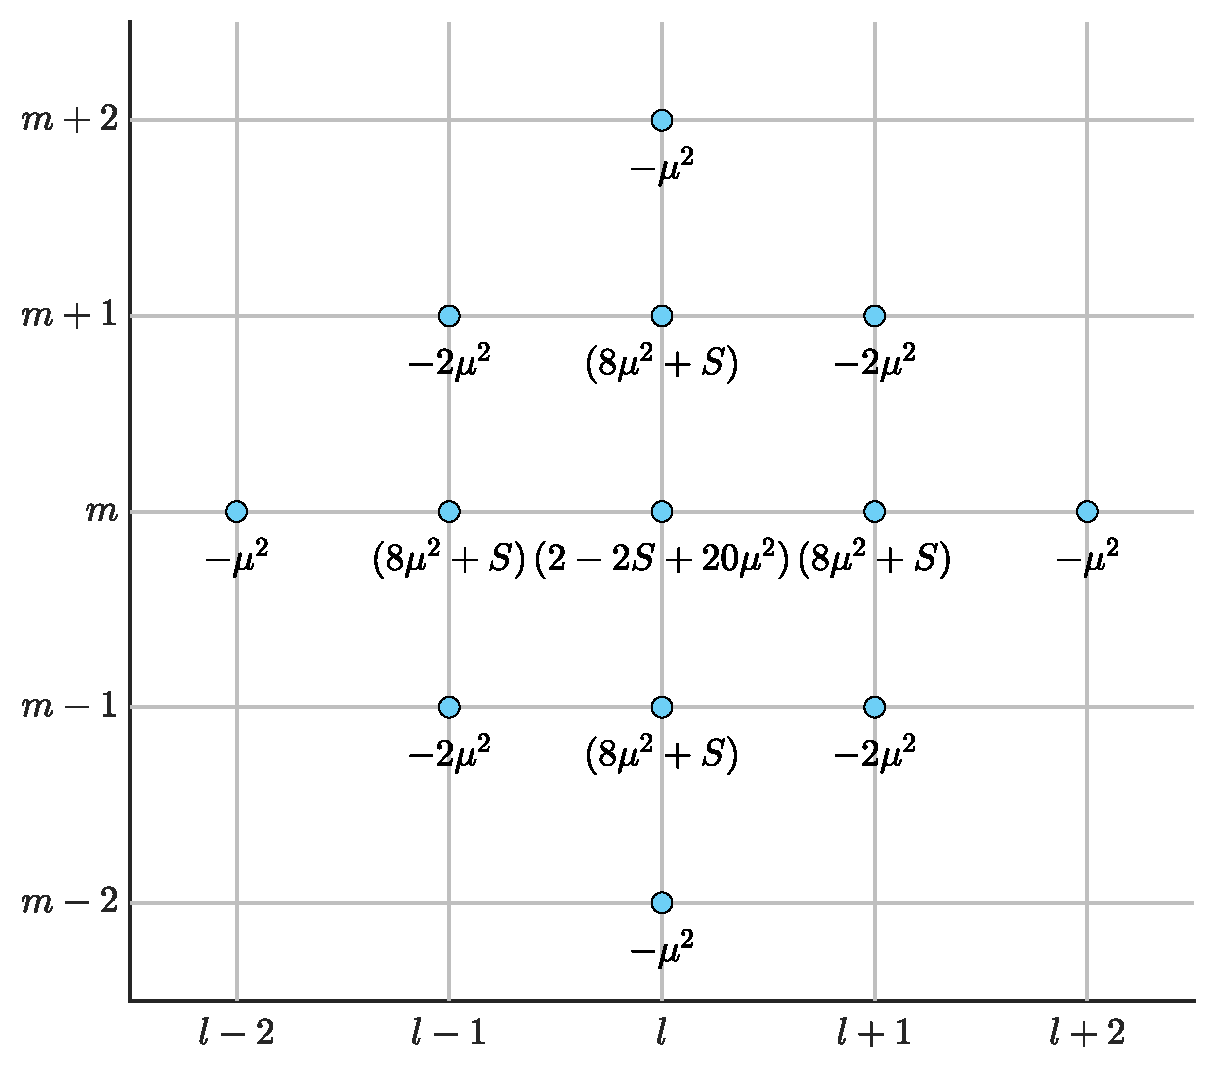
\includegraphics[width=\figWidth]{figures/resonators/2d/curPlateStencil.eps}}\hspace{\figSpacing}
    \subfloat[Stencil of $u_{l,m}^{n-1}$.\label{fig:prevStencilPlate}]{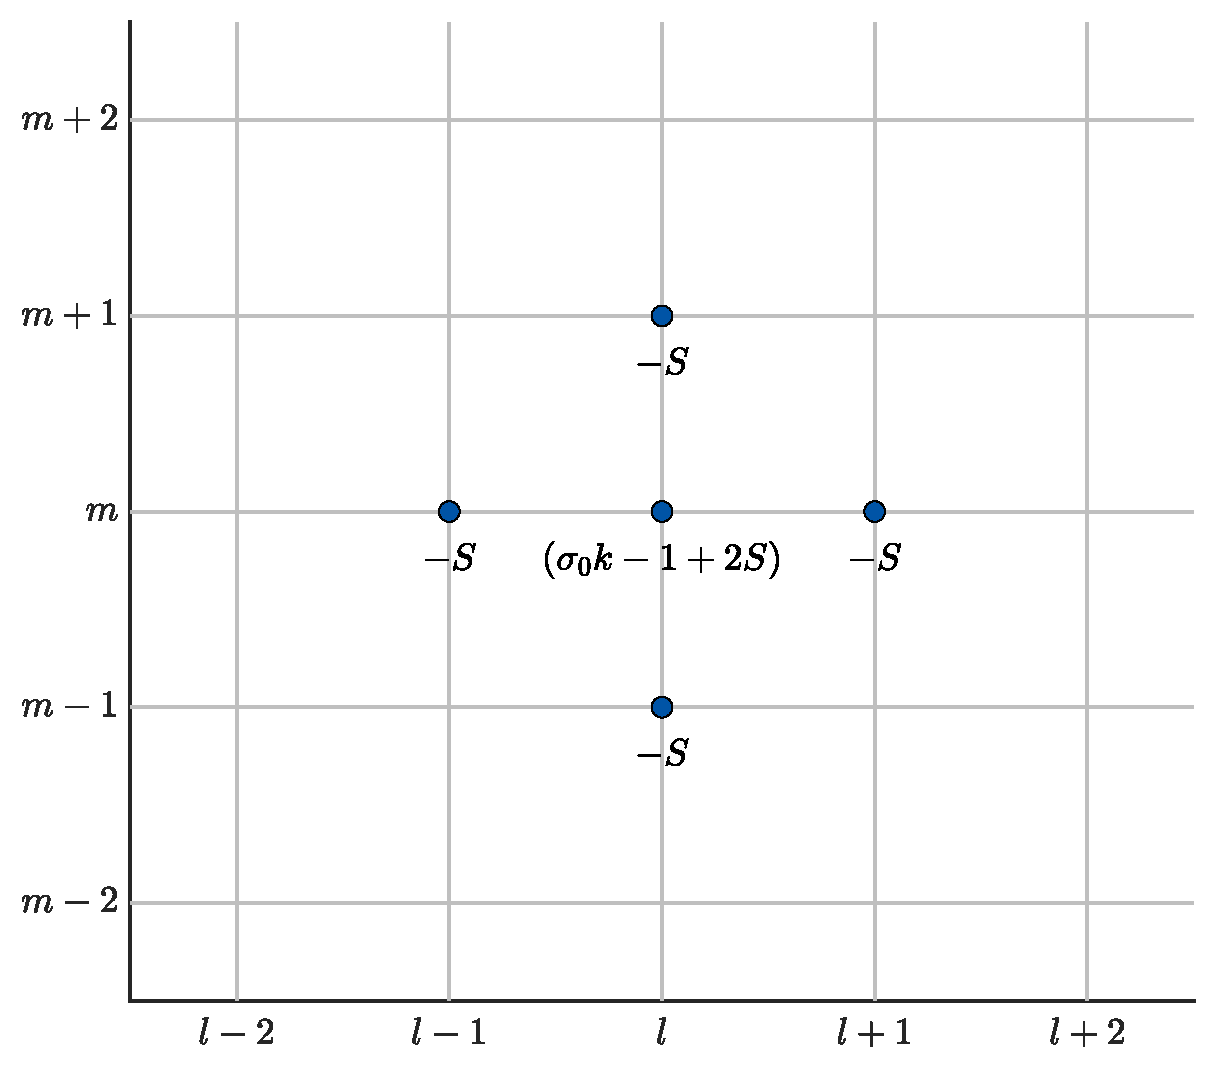
\includegraphics[width=\figWidth]{figures/resonators/2d/prevPlateStencil.eps}}
    \caption{The stencil of the plate with various parts of update equation \eqref{eq:plateUpdate} shown (using $S = 2\so k/h^2$ for brevity). (a) An overview. (b) The current time-step $n$. (c) The previous time-step $n-1$. \label{fig:plateStencil}}
\end{figure}

\subsection{Energy Analysis}
\begin{equation}
    \dtp \h = -\q 
\end{equation}
where 
\begin{equation}\label{eq:energyBalanceThinPlate}
    \begin{gathered}
        \h = \t + \v, \qwiq \t = \frac{\rho H}{2} \left\lVert\delta_{t-}\ulmn\right\rVert_{d}^2 \quad \text{and} \\
        \v = \frac{D}{2}\langle\delta_{\Delta\boxplus} \ulmn, e_{t-}\delta_{\Delta\boxplus} \ulmn\rangle_{\overline{\underline{d}}}\ .
    \end{gathered}
\end{equation}
and 
\begin{equation}\label{eq:dampingTermThinPlate}
    \mathfrak{q} = 2\sz \rho A \lVert\dtd\ulmn\rVert_d^2 - 2 \so \rho A \langle \dtd \ulmn, \dtm \delta_{\Delta\boxplus}\uln \rangle_d,
\end{equation}

\section{Stiff membrane}
Like the stiff string, the membrane can be extended with a stiffness term to yield a \textit{stiff membrane} \cite{Fletcher1998}. This model has been used for paper \citeP[F]...
Combining between Eqs. \eqref{eq:2DwavePDE} and \eqref{eq:platePDE} including the losses yields
\begin{equation}\label{eq:stiffMembrane}
    \rho H \ptt u = T\Delta u - D
    \Delta\Delta u
\end{equation}


Is essentially a 2D stiff string. 
\chapter{Brass}\label{ch:brass}

Bore

\section{Second-order system}

The first main difference between the 1D brass PDE and the 1D wave equation is the possibility of having a variable cross-section. Following Section 19.3 from \cite{Bilbao2018}, the PDE for a 1D (axially symmetric) acoustic tube with variable cross-section is (also known as \textit{Webster}'s equation)
\begin{equation}\label{eq:webstersPDE}
    S\partial_t^2\Psi = c^2\partial_x(S\partial_x\Psi),
\end{equation}
with \textit{acoustic potential} $\Psi = \Psi(x,t)$ (m$^2$/s), $S = S(x)$ is the cross sectional area (m$^2$) and wave speed $c$ (m/s).

\subsection{Discretisation}
Introducing interleaved gridpoints at $n-1/2$ and $n+1/2$ for $S$, a we can discretise Eq. \eqref{eq:webstersPDE} (following \cite{Bilbao2018}) to
\begin{equation}\label{eq:discWebster}
    \Sbar \delta_{tt}\Psi^n_l = c^2\dxp(\Sm(\delta_{x-}\Psiln)),
\end{equation}
where
\begin{equation}
    \Sbar = \mu_{t+}\Sm = \frac{\Sp + \Sm}{2}.
\end{equation}
The right side of the equation in \eqref{eq:discWebster} contains an operator applied to two grid functions ($S$ and $\Psi$) multiplied onto each other. In order to expand this, we need to use the product rule (Eq. (2.23) in \cite{theBible}) which is
\begin{equation}
    \dxp (u_lw_l) = (\dxp u_l)(\mxp{w_l}) + (\mxp u_l)(\dxp w_l).
\end{equation}
In the case of \eqref{eq:discWebster}, $u_l \triangleq \Sm$ and $w_l \triangleq \dxm\Psiln$. Expanding (retaining the notation for $\Sbar$) and solving for $\Psinp$ yields (Appendix \ref{app:webstersUpdateEq})
\begin{equation}
    \Psinp = 2(1-\lambda^2)\Psiln-\Psinm+ \frac{\lambda^2\Sp}{\Sbar}\Psilp + \frac{\lambda^2\Sm}{\Sbar}\Psilm,\label{eq:webstersUpdateEq}
\end{equation}
which is identical to Eq. (19.51) in \cite{Bilbao2018}.

\subsection{Boundary Conditions}
The choices for boundary conditions in an acoustic tube are open and closed, defined as \cite{Bilbao2018}
\begin{equation}
    \begin{split}
        \partial_t\Psi &= 0\ \text{(open, Dirichlet)}\\
        \partial_x\Psi &= 0\ \text{(closed, Neumann)},
    \end{split}
\end{equation} 
at the ends of the tube. This might be slightly counter-intuitive as in the case of a string ``closed" might imply the ``clamped" or Dirichlet boundary condition. The opposite can be intuitively shown imagining a wave front with a positive acoustic potential moving through a tube and hitting a closed end. What comes back is also a wave front with a positive acoustic potential, i.e., the sign of the potential does not flip, which also happens using the free or Neumann condition for the string.

In this case we follow \cite[Chapter 9]{theBible} and use the following
\begin{equation}\label{eq:openClosed}
    \partial_x\Psi(0, t) = 0 \quad \text{and} \quad \partial_t\Psi(L, t) = 0
\end{equation}
i.e. closed at the left end and open at the right end. In discrete time we have two choices for the closed condition
\begin{equation}\label{eq:centNonCentBound}
\begin{split}
    \delta_{x\cdot}\Psi_0^n &= 0 \ \Rightarrow \ \Psi_{-1}^n = \Psi_1^n \quad \text{(centered)}\\
    \delta_{x-}\Psi_0^n &= 0\  \Rightarrow \ \Psi_{-1}^n = \Psi_0^n\quad \text{(non-centered)}
\end{split}
\end{equation}
At the left boundary we can now solve Eq. \eqref{eq:webstersUpdateEq} for the centered case:
\begin{equation}
    \begin{aligned}
        \Psi_0^{n+1} &= 2(1-\lambda^2)\Psi_0^n-\Psi_0^{n-1}+ \frac{\lambda^2S_{1/2}}{\bar S_0}\Psi_1^n + \frac{\lambda^2S_{-1/2}}{\bar S_0}\Psi_{-1}^n\nonumber\\
        \Psi_0^{n+1} &= 2(1-\lambda^2)\Psi_0^n-\Psi_0^{n-1}+ \frac{\lambda^2(S_{1/2}+S_{-1/2})}{\bar S_0}\Psi_1^n\nonumber\\
         \Psi_0^{n+1} &= 2(1-\lambda^2)\Psi_0^n-\Psi_0^{n-1}+ 2\lambda^2\Psi_1^n,
    \end{aligned}
\end{equation}
and the non-centered case
\begin{equation}\label{eq:nonCentLeft}
    \Psi_0^{n+1} = 2(1-\lambda^2)\Psi_0^n-\Psi_0^{n-1}+ \frac{\lambda^2S_{1/2}}{\bar S_0}\Psi_1^n + \frac{\lambda^2S_{-1/2}}{\bar S_0}\Psi_0^n.
\end{equation}
As can be seen from the equations above, we need undefined points $\bar S_0$ and $S_{-1/2}$. At the left boundary, we set $\bar S_0 = S_0$ from which, we can calculate $S_{-1/2}$:
\begin{equation}
        S_0 = \frac{1}{2}(S_{1/2} + S_{-1/2}) \ \Rightarrow \  S_{-1/2}
        = 2S_0 - S_{1/2}
\end{equation}
The same can be done for the right boundary ($\bar S_N = S_N$) if this is chosen to be anything else but open (e.g., closed or radiating -- see Section \ref{sec:radiating}):
\begin{equation}
    S_N = \frac{1}{2}(S_{N+1/2} + S_{N-1/2}) \ \Rightarrow \ S_{N+1/2} = 2S_N - S_{N-1/2}.
\end{equation}
For now though, we follow the conditions given in \eqref{eq:openClosed} and we can simply set the right boundary to its initial state
\begin{equation}
    \Psi_N^n = \Psi_N^0
\end{equation}
which is normally $0$. A more realistic open end is a radiating one, which can be found below.
\subsubsection{Radiating end}\label{sec:radiating}
We can change the condition presented in Eq. \eqref{eq:openClosed} to a radiating end,
\begin{equation}\label{eq:radCont}
    \partial_x\Psi(L,t) = -a_1\partial_t\Psi(L,t)-a_2\Psi(L,t)
\end{equation}
where \cite{theBible}
\begin{equation}
    a_1 = \frac{1}{2(0.8216)^2c} \quad \text{and} \quad a_2 = \frac{L}{0.8216\sqrt{S_0S(1)/\pi}}.
\end{equation}
taken from \cite{Atig2004} and are valid for a tube terminating on an infinite plane. The terms in Eq. \eqref{eq:radCont} are a damping and an inertia term where $a_1$ is a loss coefficient (in s/m) and $a_2$ is the \textbf{inertia coefficient} (in m$^{-1}$). The centered and non-centered case are defined as
\begin{equation}\label{eq:rightBoundaryConditions}
\begin{split}
    \delta_{x\cdot}\Psi_N^n &= 0 \ \Rightarrow \ \Psi_{N+1}^n = \Psi_{N-1}^n \quad \text{(centered)}\\
    \delta_{x+}\Psi_N^n &= 0\  \Rightarrow \ \Psi_{N+1}^n = \Psi_N^n\qquad \text{(non-centered)}
\end{split}
\end{equation}
First, we solve Eq. \eqref{eq:radCont} for the centered (Eq. (9.16) in \cite{theBible})
\begin{equation}\label{eq:centRadBound}
    \delta_{x\cdot}\Psi_N^n = -a_1\dtd\Psi_N^n - a_2\mu_{t\cdot}\Psi_N^n
\end{equation}
which can be expanded and solved for $\Psi_{N+1}^n$ according to
\begin{align}
    \frac{1}{2h}(\Psi_{N+1}^n - \Psi_{N-1}^n) &= -\frac{a_1}{2k}(\Psi_N^{n+1} - \Psi_N^{n-1}) - \frac{a_2}{2}(\Psi_N^{n+1} + \Psi_N^{n-1})\nonumber\\
    \Psi_{N+1}^n &= h\left(-\frac{a_1}{k}(\Psi_N^{n+1} - \Psi_N^{n-1}) - a_2(\Psi_N^{n+1} + \Psi_N^{n-1})\right) + \Psi_{N-1}^n,
\end{align}
which can be substituted into Eq. \eqref{eq:webstersUpdateEq} (Appendix \ref{app:centeredRad}) 
\begin{equation}
    \Psi_N^{n+1} = \frac{2(1-\lambda^2)\Psi_N^n-\Psi_N^{n-1}+\frac{h\lambda^2S_{N+1/2}}{\bar S_N}\left(\frac{a_1}{k}-a_2\right)\Psi_N^{n-1} + 2\lambda^2\Psi_{N-1}^n}{\left(1+\left(\frac{a_1}{k}+a_2\right)\frac{h\lambda^2S_{N+1/2}}{\bar S_N}\right)}.
\end{equation}
The same can be done for the non-centered case (Eq. (9.15) in \cite{theBible})
\begin{equation}\label{eq:nonCentRadBound}
    \delta_{x+}\Psi_N^n = -a_1\dtd\Psi_N^n - a_2\mu_{t\cdot}\Psi_N^n
\end{equation}
which when solved for $\Psi_{N+1}^n$ yields
\begin{align}
    \frac{1}{h}(\Psi_{N+1}^n - \Psi_{N}^n) &= -\frac{a_1}{2k}(\Psi_N^{n+1} - \Psi_N^{n-1}) - \frac{a_2}{2}(\Psi_N^{n+1} + \Psi_N^{n-1})\nonumber\\
        \Psi_{N+1}^n &= h\left(-\frac{a_1}{2k}(\Psi_N^{n+1} - \Psi_N^{n-1}) - \frac{a_2}{2}(\Psi_N^{n+1} + \Psi_N^{n-1})\right) + \Psi_{N}^n.
\end{align}
Substituted into Eq. \eqref{eq:webstersUpdateEq} yields (Appendix \ref{app:nonCentRad})
\begin{equation}
    \Psi_N^{n+1} = \frac{2(1-\lambda^2)\Psi_N^n-\Psi_N^{n-1}+\frac{h\lambda^2S_{N+1/2}}{\bar S_N}\left(\frac{a_1}{2k}-\frac{a_2}{2}\right)\Psi_N^{n-1} + \frac{\lambda^2S_{N+1/2}}{\bar S_N}\Psi_{N}^n + \frac{\lambda^2S_{N-1/2}}{\bar S_N}\Psi_{N-1}^n}{\left(1+\left(\frac{a_1}{2k}+\frac{a_2}{2}\right)\frac{h\lambda^2S_{N+1/2}}{\bar S_N}\right)}.
\end{equation}

\section{First-order system}

This will be the first appearance of a first-order system. 




\part{Exciters}\label{part:exciters}
\chapter*{Exciters}
Several resonators have been introduced in part \ref{part:resonators}, different mechanisms to excite them will be introduced here. First, different examples of 

and have a great effect on the eventual timbre of the sound. 
Chapter \ref{ch:physInspExcitations} presents various physically inspired excitations some of which made a brief appearance in Part \ref{part:resonators}. Chapter \ref{ch:bow} introduces a static and a dynamic friction model that can be used for bowing resonators. Additionally, this chapter presents the contribution made in \citeP[C]: the elasto-plastic friction model applied to FDTD stiff strings. Finally, Chapter \ref{ch:lipreed} presents the lip reed as a way to excite brass instruments. 

% \chapter{Unmodelled Excitations}\todo{Different title here?}

\section{Initial conditions}

\subsubsection{Hammer}
Full raised cosine

\subsubsection{Pluck}
\begin{itemize}
    \item Cut-off raised cosine
    \item Triangle (for string)
\end{itemize}


\section{Signals}
\subsection{Pulse train}
For brass

\subsection{Noise}
Noise input

\chapter{Excitations}\label{ch:excitations}

\section{Unmodelled excitations}

\subsection{Impulse}
The simplest way of exciting a system is to add an impulse to 
\subsection{The raised cosine}


\subsubsection{Pluck}
\begin{itemize}
    \item Cut-off raised cosine
    \item Triangle (for string)
\end{itemize}

\subsection{Signals}
\subsubsection{Pulse train}
For brass

\subsubsection{Noise}
Noise input

\section{Preamble: Newton-Raphson}\label{sec:newtonRaphson}
Before moving on to more complex excitation mechanisms, it is useful to go over the process of how to solve some of these. 
Iterative root-finding method that finds answers to nonlinear equations. 

\subsection{Mass-spring Systems Revisited: Adding Damping}

Damping can be added to Eq. \eqref{eq:massSpringPDE}  
\begin{equation}
    M\ddot u = -Ku - R\dot u
\end{equation}
with damping coefficient $R$ (in kg/s). To this system we can add an external force:
\begin{equation}
    M\ddot u = -Ku - R\dot u + F
\end{equation}
where 
\section{The Bow}
The bow

Excites the system with a force due to friction, which has a nonlinear relationship to the relative velocity between the bow and the string. 



Helmholtz motion..

\begin{figure}[h]
    \centering
    \begin{tikzpicture}[->,node distance=3cm,
        thick,main node/.style={circle,draw}]
    
        \node[] (image) at (0,0) {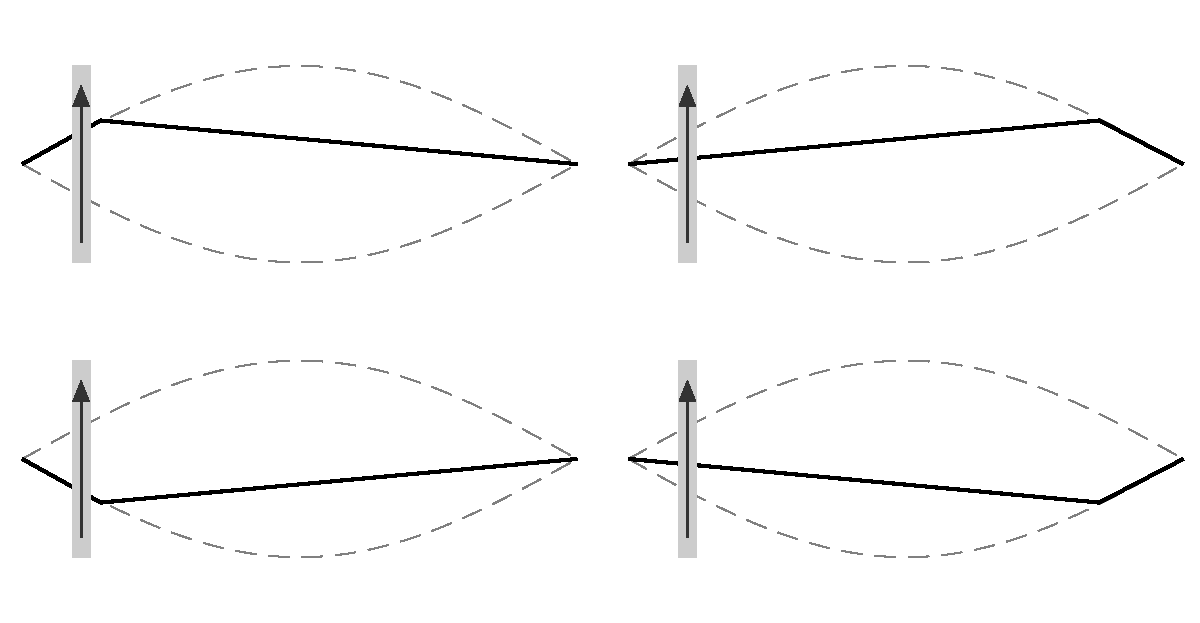
\includegraphics[width=1\columnwidth]{figures/exciters/helmholtz.eps}};
    
        \draw[thick, ->] (-0.25,0.60) arc (110:430:0.6);
        
      \end{tikzpicture}
    \caption{Helmholtz motion. \label{fig:helmholtz}}
\end{figure}

coined as `stick-slip' motion by Bowden and Leben in 1939 \cite{Bowden1939}

See fx. \url{https://www.youtube.com/watch?v=6JeyiM0YNo4}

Characteristic triangular motion (wave shapes?)

\subsection{Static Friction Models}
In static bow-string-interaction models, the friction force is defined as a function of the relative velocity between the bow and the string only.
The first mathematical description of friction was proposed by Coulomb in 1773 \cite{Coulomb1773}\todo{check references here} to which static friction, or \textit{stiction}, was added by Morin in 1833 \cite{Morin1833} and viscous friction, or velocity-dependent friction, by Reynolds in 1886 \cite{Reynolds1886}. In 1902, Stribeck found a smooth transition between the static and the coulomb part of the friction curve now referred to as the Stribeck effect \cite{Stribeck1902}. The latter is still the standard for static friction models today.

In this project, only the following static friction model has been used \cite{theBible}

\begin{equation}\label{eq:frictionCharacteristic}
    \Phi (\vrel) = \sqrt{2a}\vrel e^{-a\vrel^2 + 1/2}
\end{equation}

\todo{FULL DOC SWEEP: check figure centering}\begin{figure}[h]
    \centering
    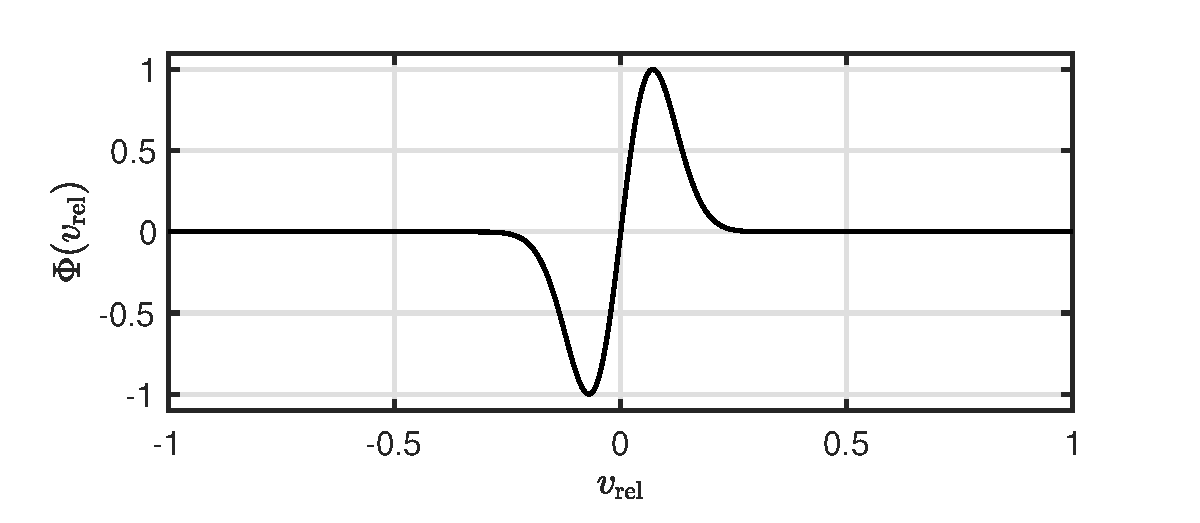
\includegraphics[width=0.8\textwidth]{figures/exciters/frictionCharacteristic.eps}
    \caption{The friction characteristic in \eqref{eq:frictionCharacteristic} with $a = 100$. \label{fig:frictionCharacteristic}}
\end{figure}

\subsection{Dynamic Friction Models}
As opposed to less complex bow models, such as the hyperbolic [source] and exponential [source] models, the elasto-plastic bow model assumes that the friction between the bow and the string is caused by a large quantity of bristles, each of which contributes to the total amount of friction.

Dynamic friction models exhibit \SWcomment[/ model] \textit{hysteresis}: the dependence of a system on its history. 
\begin{figure}[ht]
    \centering
    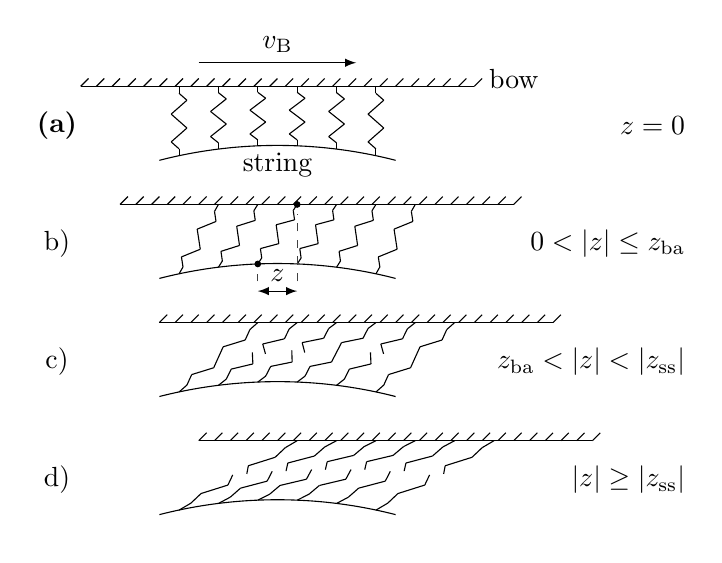
\begin{tikzpicture}
    
    \def\radius{6}; % Radius of the string (>2!)
    \pgfmathsetmacro{\reps}{3}; % How may back-and-forths in the drawing of the springs
    \def\horShift{0.5}; %how far the bow is shifted to the right in b)
    \def\bowSpacing{0.2};
    \def\drawingSpacing{1.5}
    \def\bowWidth{5};
    
    %subfigure letters
    \node (A) at (-2.8, 0.5) {\textbf{(a)}};
    \node (B) at (-2.8, 0.5 - \drawingSpacing) {b)};
    \node (C) at (-2.8, 0.5 - \drawingSpacing * 2) {c)};
    \node (D) at (-2.8, 0.5 - \drawingSpacing * 3) {d)};
    
    %bow velocity arrow
    \draw[->] (-1, 1.3) -- (1, 1.3) node [midway, above] (velText) {$v_\text{B}$};
    
    \pgfmathsetmacro{\zCoordTop}{0};
    \pgfmathsetmacro{\zYCoordBottom}{0};
    \def\springForZ{2}
    \foreach \drawing in {0, ..., 3}
    {
        %% Draw String
        \begin{scope}
            \clip (-1.5,-0.2- \drawing * \drawingSpacing) rectangle (1.5,1.5);
            \draw (0,-\radius + 0.25 - \drawing * \drawingSpacing) circle(\radius);
        \end{scope}

        %% Draw Bow
        \def\halfBW{\bowWidth*0.5}
        \pgfmathsetmacro{\halfNumDiag}{0.5 * \bowWidth / \bowSpacing};
        \draw[-] (-\halfBW + \drawing * \horShift,1 - \drawing * \drawingSpacing) -- (\halfBW + \drawing * \horShift, 1 - \drawing * \drawingSpacing);
        \foreach \bowDiag in {-\halfNumDiag, ...,\halfNumDiag}
        {
        \pgfmathtruncatemacro{\bD}{\bowDiag}
        % \ifnum\drawing=0
        %     \ifnum\bD<-1
        %         \draw[-] (\drawing * \horShift + \bowDiag * \bowSpacing, -\drawing * \drawingSpacing + 1) -- (\drawing * \horShift + \bowDiag * \bowSpacing + 0.1, -\drawing * \drawingSpacing + 0.1 + 1);
        %         \else
        %         \ifnum\bD>1
        %             \draw[-] (\drawing * \horShift + \bowDiag * \bowSpacing, -\drawing * \drawingSpacing + 1) -- (\drawing * \horShift + \bowDiag * \bowSpacing + 0.1, \drawing * -2 + 0.1 + 1);
        %         \fi
        %     \fi
        % \else
            \draw[-] (\drawing * \horShift + \bowDiag * \bowSpacing, -\drawing * \drawingSpacing + 1) -- (\drawing * \horShift + \bowDiag * \bowSpacing + 0.1, -\drawing * \drawingSpacing + 0.1 + 1);
        % \fi
            
        }
        
        \def\brokenSprings{{0, 1, 1, 0, 1, 0}};
        %% Draw Springs
        \foreach \springNo in {0, ..., 5}
        {
            % Calculate spring length depending on the radius of the string
            \pgfmathsetmacro{\startX}{\springNo  * 0.5 - 1.25};
            \pgfmathsetmacro{\calcSpace}{(\radius + 1) - \radius * sin(acos(\startX/\radius)) - 0.25};
            \pgfmathsetmacro{\springLength}{sqrt(\calcSpace*\calcSpace+\drawing*\horShift*\drawing*\horShift)};
            
            \pgfmathsetmacro{\spacing}{\springLength / (\reps + 2)}; 
            % spacing between two spring-back-and-forths
            \ifnum\drawing=0
                \pgfmathsetmacro{\rot}{0};
            \else
                \pgfmathsetmacro{\rot}{(270+(atan(\calcSpace/(\drawing*\horShift))))}; %rotation of the springs
            \fi
            
            \ifnum\drawing=1
                \ifnum\springNo=\springForZ
                    \pgfmathsetmacro{\resTwo}{sqrt(\springLength*\springLength-\horShift*\horShift)};
                    \global\let\zCoordBottom = \resTwo;
                \fi
            \fi
        
            \pgfmathsetmacro{\isBroken}{\brokenSprings[\springNo]};
            % debug code
            % \node (nodeTest\springNo) at (\springNo*1.1-2, -3 - 1 * \drawing + 0.3 * \springNo) {\isBroken};
            
            \begin{scope}[shift={(\startX + \drawing * \horShift,1 -\drawing * \drawingSpacing)}]
                \pgfmathsetmacro{\xWidth}{0.1 - (\drawing * 0.02)};
                \draw[-, rotate = \rot] (0, 0) -- (0, -\spacing * 0.5);
                \draw[-, rotate = \rot] (0, -\spacing * 0.5) -- (\xWidth, -\spacing);
                \def\Y{-\spacing}
                \foreach \idx in {1,...,\reps}
                {
                    \pgfmathsetmacro{\idxMinOne}{\idx-1};
                    \ifnum\drawing=2
                        \ifnum\isBroken=1
                            \pgfmathtruncatemacro{\idxT}{\reps * 0.5 + 1}
                            \ifnum\idx=\idxT
                                \draw[-, rotate = \rot] (\xWidth, \Y - \idxMinOne * \spacing) -- (-\xWidth,\Y - \idx * \spacing*0.6);
                                \draw[-, rotate = \rot] (\xWidth, \Y - \idxMinOne * \spacing * 1.66) -- (-\xWidth,\Y - \idx * \spacing);
                            \else
                                \draw[-, rotate = \rot] (\xWidth, \Y - \idxMinOne * \spacing) -- (-\xWidth,\Y - \idx * \spacing);
                            \fi
                        \else
                                \draw[-, rotate = \rot] (\xWidth, \Y - \idxMinOne * \spacing) -- (-\xWidth,\Y - \idx * \spacing);
                        \fi
                    \else
                        \ifnum\drawing=3
                            \pgfmathtruncatemacro{\idxT}{\reps * 0.5 + 1}
                            \ifnum\idx=\idxT
                                \draw[-, rotate = \rot] (\xWidth, \Y - \idxMinOne * \spacing) -- (-\xWidth,\Y - \idx * \spacing*0.6);
                                \draw[-, rotate = \rot] (\xWidth, \Y - \idxMinOne * \spacing * 1.66) -- (-\xWidth,\Y - \idx * \spacing);
                            \else
                                \draw[-, rotate = \rot] (\xWidth, \Y - \idxMinOne * \spacing) -- (-\xWidth,\Y - \idx * \spacing);
                            \fi
                        \else
                            \draw[-, rotate = \rot] (\xWidth, \Y - \idxMinOne * \spacing) -- (-\xWidth,\Y - \idx * \spacing);
                        \fi
                    \fi
                    \pgfmathsetmacro{\invXWidth}{\xWidth*-1};
                    \global\let\xWidth = \invXWidth;
                    \pgfmathsetmacro{\lastYPre}{\Y - \idx * \spacing};
                    \global\let\lastY = \lastYPre;
                }
                \draw[-, rotate = \rot] (\xWidth, \lastY) -- (0, \lastY - \spacing * 0.5);
                \draw[-, rotate = \rot] (0, \lastY - \spacing * 0.5) -- (0, \lastY - \spacing);
             \end{scope}
             
        }
        % \draw[<->] (2,2-0.707) -- node[right] {$r=\sqrt{2} \Rightarrow A=\pi(\sqrt{2})^2=2\pi$} (2,2+0.707);
        
        % \node(stringText) at (0, -\drawing * 2) {string};
        % \node[block, minimum height = 0.15cm, fill=white, draw=white] (bowText) at (\drawing * \horShift, 1.23 - \drawing * 2) {bow};
    }
    \filldraw[black] (-1.25+\springForZ*0.5 + \horShift,1-\drawingSpacing) circle (1pt) node[anchor=center](topZ){};
    \filldraw[black] (-1.25++\springForZ*0.5,1-\zCoordBottom-\drawingSpacing) circle (1pt) node[anchor=center](bottomZ){};
    
    \node [](leftNode) at (-1.25+\springForZ*0.5,-\drawingSpacing - 0.1) {};
    \node [](rightNode) at (-1.25 +\springForZ*0.5 + \horShift,-\drawingSpacing - 0.1) {};
    
    \draw[<->] (leftNode.center) -- (rightNode.center) node [midway, above] (TextNode) {$z$};
    \draw[dashed, darkgray] (leftNode) -- (bottomZ);
    \draw[dashed, darkgray] (rightNode) -- (topZ);
    %% Draw bow and string texts
        \node(stringText) at (0, 0) {string};
        \node(bowText) at (3, 1.1) {bow};
    %% Draw descriptions of z
    \def\zTexts{{"$z=0$", "$0<|z|<z_{\text{ba}}$", "$z_{\text{ba}}<|z|< z_\text{ss}$", "$|z|>z_\text{ss}$"}};
    
    \node[anchor = east](zText1) at (5.3, 0.5) {$z=0$};
    \node[anchor = east](zText1) at (5.3, 0.5 - \drawingSpacing) {$0<|z|\leq z_{\text{ba}}$};
    \node[anchor = east](zText1) at (5.3, 0.5 - \drawingSpacing * 2) {$z_{\text{ba}}<|z|< |z_\text{ss}|$};
    \node[anchor = east](zText1) at (5.3, 0.5 - \drawingSpacing * 3) {$|z|\geq|z_\text{ss}|$};
    
    \end{tikzpicture}
    \caption{\it Microscopic displacements of the bristles between the bow and the string. The bow moves right with a velocity of $v_\text{B}$. (a) The initial state is where the average bristle displacement $z=0$. (b) The bow has moved right relative to the string. The purely elastic, or presliding regime is entered (stick). (c) After the break-away displacement $z_\text{ba}$, more and more bristles start to `break'. This is defined as the elasto-plastic regime. (d) After all bristles have `broken', the steady state (slip) is reached and the purely plastic regime is entered. (Taken from \citeP[C].)\SWcomment[exactly the same caption as paper]}
    \label{fig:elastoPlastic}
\end{figure}

\section{Lip-reed}
Lip-reed model



Coupling to Tube


\part{Interactions}\label{part:interactions}
\chapter*{Exciters}
Several resonators have been introduced in part \ref{part:resonators}, different mechanisms to excite them will be introduced here. First, different examples of 

and have a great effect on the eventual timbre of the sound. 
Chapter \ref{ch:physInspExcitations} presents various physically inspired excitations some of which made a brief appearance in Part \ref{part:resonators}. Chapter \ref{ch:bow} introduces a static and a dynamic friction model that can be used for bowing resonators. Additionally, this chapter presents the contribution made in \citeP[C]: the elasto-plastic friction model applied to FDTD stiff strings. Finally, Chapter \ref{ch:lipreed} presents the lip reed as a way to excite brass instruments. 

\chapter{Connections}\label{ch:connections}
Many musical instruments consist of multiple subsystems like the ones presented in Part \ref{part:resonators}. For example, one could simulate a guitar by modelling six separate instances of the stiff string presented in Chapter \ref{ch:stiffString}, and the sound board (as a simplified instrument body), using a thin plate presented in Section \ref{sec:thinPlate}. 
The interaction between the strings and the body can then be modelled using \textit{connections}. %Apart from interactions between resonators, one could use connections for instrument control. For example, one could connect a mass-spring-damper system to a string, to simulate a point-like damping finger to create different pitches.

Examples of connected resonators based on FDTD methods are shown in e.g. \cite{theBible} and \cite{Bilbao2009Modular}. The latter presents a modular approach to connect any number of resonators in arbitrary ways using an extremely compact matrix form of the entire system.
% Although briefly mentioned in the previous chapter in Section \ref{sec:twoSidedCollision}

The first example presented in this chapter is the case of two ideal strings, connected using a rigid and spring-like connection. Afterwards, the connection between a stiff string and a thin plate using a nonlinear spring will be presented, and has been used extensively in papers \citeP[A] and \citeP[B]. Before moving on to these examples, interpolation and spreading operators in 2D will be introduced.

\section{Interpolation and spreading in 2D}\label{sec:interpolationSpreading2D}
This section summarises and extends \cite[Sec. 10.2.1, pp. 293--294]{theBible}.

One can extend the interpolation and spreading operators presented in Section \ref{sec:interpolationSpreading} to 2D by adding an additional argument to the operators. Using $l_\itxt = \floor[x_\itxt / h]$ and $m_\itxt = \floor[y_\itxt / h]$, a $0$\thOrder interpolation operator $I_0(x_\itxt, y_\itxt) = I_{(l, m), 0}(x_\itxt, y_\itxt)$ is defined as
\begin{equation}
    I_0(x_\itxt, y_\itxt) = \begin{cases}
        1, & \text{if } l = l_\itxt \text{ and } m = m_\itxt,\\
        0, & \text{otherwise}.
    \end{cases}
\end{equation}
Notice that the same value for the grid spacing $h$ is used for both the $x$ and $y$ direction.

Using the fractional part of the flooring operations $\alpha_x = x_\itxt/h - l_\itxt$ and $\alpha_y= y_\itxt/h - m_\itxt$, a 2D linear interpolator  $I_1(x_\itxt, y_\itxt) = I_{(l, m), 1}(x_\itxt, y_\itxt)$ can then be composed as
\begin{equation}
    I_1(x_\itxt, y_\itxt) = \begin{cases}
        (1 - \alpha_x)(1 - \alpha_y)& \text{if } l = l_\itxt \text{ and } m = m_\itxt, \\
        (1 - \alpha_x)\alpha_y& \text{if } l = l_\itxt \text{ and } m = m_\itxt + 1, \\
        \alpha_x(1 - \alpha_y)& \text{if } l = l_\itxt + 1 \text{ and } m = m_\itxt, \\
        \alpha_x\alpha_y& \text{if } l = l_\itxt+1 \text{ and } m = m_\itxt+1, \\
        0, & \text{otherwise}.
    \end{cases}
\end{equation}

Spreading operators are defined in the same way as in Section \ref{sec:interpolationSpreading}. A $0$\thOrder spreading operator $J_0(x_\itxt, y_\itxt) = J_{(l,m),0}(x_\itxt, y_\itxt)$ can be defined as
\begin{equation}
    J_0(x_\itxt, y_\itxt) = \frac{1}{h^2}\begin{cases}
        1, & \text{if } l = l_\itxt \text{ and } m = m_\itxt,\\
        0, & \text{otherwise},
    \end{cases}
\end{equation}
as well as a linear spreading operator $J_1(x_\itxt, y_\itxt) = J_{(l,m),1}(x_\itxt, y_\itxt)$ as
\begin{equation}
    J_1(x_\itxt, y_\itxt) = \frac{1}{h^2}\begin{cases}
        (1 - \alpha_x)(1 - \alpha_y)& \text{if } l = l_\itxt \text{ and } m = m_\itxt, \\
        (1 - \alpha_x)\alpha_y& \text{if } l = l_\itxt \text{ and } m = m_\itxt + 1, \\
        \alpha_x(1 - \alpha_y)& \text{if } l = l_\itxt + 1 \text{ and } m = m_\itxt, \\
        \alpha_x\alpha_y& \text{if } l = l_\itxt+1 \text{ and } m = m_\itxt+1, \\
        0, & \text{otherwise}.
    \end{cases}
\end{equation}
Notice that the scaling is by $1/h^2$ (due to the 2D system) rather than $1/h$ in the 1D case. Some intuition on this will be given below. 

As in the 1D case, the spreading operator approximates a spatial Dirac delta function, which -- in 2D -- is defined as 
\begin{equation}\label{eq:spatialDirac2D}
    \delta(x,y)= \begin{cases}
        \infty, & x = y = 0,\\
        0, & \text{otherwise},
    \end{cases} \qaq \int_{-\infty}^{\infty} \int_{-\infty}^{\infty} \delta(x,y)dxdy = 1.
\end{equation}
where $\delta(x,y)$ has units of m$^{-2}$. Again, as described in Section \ref{sec:interpolationSpreading}, this definition will be approximated by spreading operators, rather than be used directly. 

\subsection{Alternative interpretation of grid points}\label{sec:alternativeInterp}
Section \ref{sec:gridFunctions} gives an introduction to how a continuous 1D system is subdivided into grid points in space (see Figure \ref{fig:gridExp}) through the discretisation process. An alternative way to see grid points after discretisation is shown in Figure \ref{fig:gridExp2}. Rather than grid `points' with a spacing $h$ between them, a continuous system is divided into grid `sections' of length $h$. This interpretation allows for the `weight' of a grid point to be calculated from its material properties and geometry. Notice that boundaries have a length of $h/2$ such that the total length $L = Nh$ m.

As an example, the weight of one grid point (or now rather grid section) of a string can be calculated as $\rho A h$. The weight of one grid point of a 2D system can be calculated as $\rho H h^2$. As these grid points interact with each other, the forces resulting from this interaction will be scaled by their respective weight per grid point as will be shown in Section \ref{sec:stringPlateConnection}.
This interpretation hopefully provides a better intuition for the interactions between components shown in this chapter. 

\begin{figure}[h]
    \centering
    % \subfloat[If $N=5$ there are 5 sections of length $h$ and 6 grid points describing the state of the system ($l=\{0, \hdots, 5\}$).\label{fig:gridExp1}]{\includegraphics[width=0.45\textwidth]{figures/fdtd/gridExplanation.pdf}}\hspace{0.06\textwidth}
    % \subfloat[If $N$ is large (as is usually the case), The 1D system is divided into $N$ sections of length $h$ and $l=\{0, \hdots, N\}$.\label{fig:gridExp2}]{\includegraphics[width=0.45\textwidth]{figures/fdtd/gridExplanation2.pdf}}
    \includegraphics[width=0.75\textwidth]{figures/fdtd/gridFigure2.pdf}
    \caption{Alternative interpretation of the discretisation of $u(x,t)$ to a grid function $\uln$. The continuous system is divided into $N-1$ sections of length $h$ plus $2$ sections of length $h/2$ at the boundaries. Through this interpretation, the `weight' of a grid point can be calculated from its physical parameters. \label{fig:gridExp2}}
\end{figure}

\section{Connected ideal strings}\label{sec:connIdealStrings}
When working with multiple interacting systems, one finds that notation becomes extremely important. Subscripts will be extensively used in the following for extra clarity, and although this results in something of a notational jungle, it is better to be explicit and avoid confusion in the end.

As a test case for the following sections, consider two ideal strings\footnote{Recall that the ideal string is the 1D wave equation with $c=\sqrt{T/\rho A}$.} of length $L_u$ and $L_w$ (both in m) their transverse displacement denoted as $u=u(x,t)$ and $w = w(\chi,t)$ (both in m) respectively (see Section \ref{sec:1DWave}).  The systems are defined for $x\in \D_u$ with domain $\D_u=[0,L_u]$ and $\chi \in \D_w$ with domain $\D_w=[0,L_w]$ respectively. Notice that $\chi$ is used as the spatial coordinate for $w$ to denote that the two systems use different coordinate systems. Connecting these systems at $x_\ctxt\in \D_u$ and $\chi_\ctxt\in\D_w$ yields the following system of PDEs:
\begin{subequations}\label{eq:conn1DwavePDE}
    \begin{align}
        \rho_u A_u \ptt u &= T_u \pxx u -\delta(x-x_\ctxt)f, \label{eq:conn1DwavePDEu} \\
        \rho_w A_w \ptt w &= T_w \partial_\chi^2 w + \delta(\chi-\chi_\ctxt)f,\label{eq:conn1DwavePDEw}
    \end{align}
\end{subequations}
where subscripts $u$ and $w$ denote whether a variable belongs to system $u$ or $w$ respectively. Notice that the $\partial_\chi$ in Eq. \eqref{eq:conn1DwavePDEw} denotes a partial derivative with respect to $\chi$ and is an identical operation to $\px$, but on a different coordinate system. Furthermore, $f = f(t)$ is the connection force (in N) which should be equal and opposite for the connected systems according to Newton's third law (hence the inverse signs). The definition for $f$ depends on the connection type, and two alternatives will be given shortly. Finally, the spatial Dirac delta function $\delta$ is defined as in Eq. \eqref{eq:spatialDirac}, and localises the connection force along the systems. 
% The relative displacement between the two systems at their respective connection locations (in m) is defined as 
% \begin{equation}
%     \eta(t) = u(x_\text{c},t) - w_(\chi_\ctxt),
% \end{equation}
% and will be used later on. 

\subsubsection{Relative location of objects}
As explained in Chapter \ref{ch:collisions} it is important to keep in mind the relative location of two interacting objects, as this will affect the signs of the force terms added to the PDEs. As opposed to the case of collisions, the connection will have a negative effect on the object `above' and a positive effect on the one `below' due to the `pulling' behaviour of a connection.
From the signs of the force terms in system \eqref{eq:conn1DwavePDE}, it can thus be concluded that $u$ has been placed above $w$. If $f$ is positively dependent on $\eta$ (the relative displacement between the two objects at their respective connection locations), this will be defined as the object below subtracted from the object above. For system \eqref{eq:conn1DwavePDE} this will be
\begin{equation}
    \eta(t) = u(x_\text{c}, t) - w(\chi_\text{c}, t),
\end{equation}
and will be used for a spring connection in Section \ref{sec:springConnection}.

\subsection{Discrete time}
One can then discretise the state variables $u$ and $w$ to grid functions $\uln$ and $\wmn$, using $x = lh_u$ and $\chi = mh_w$, where $l\in \{0, \hdots, N_u\}$ and $m\in \{0, \hdots, N_w\}$.\footnote{Here, $m$ is used for the spatial index of $\wmn$ to avoid double subscripts $l_u$ and $l_w$.} Also see Section \ref{sec:gridFunctions}. Furthermore, $h_u$ and $h_w$ are the values of the grid spacing (both in m) and $N_u+1$ and $N_w+1$ are the number of grid points for $\uln$ and $\wmn$ respectively. Dividing Eqs. \eqref{eq:conn1DwavePDEu} and \eqref{eq:conn1DwavePDEw} by $\rho_u A_u$ and $\rho_w A_w$ respectively, yields
\begin{subequations}\label{eq:conn1DwaveFDS}
    \begin{align}
        \dtt \uln &= c_u^2 \dxx \uln -\Ju\frac{f^n}{\rho_u A_u}, \label{eq:conn1DwaveFDSu} \\
        \dtt \wmn &= c_w^2 \delta_{\chi\chi} \wmn + \Jw\frac{f^n}{\rho_w A_w},\label{eq:conn1DwaveFDSw}
    \end{align}
\end{subequations}
where $c_u = \sqrt{T_u / \rho_uA_u}$ and $c_w = \sqrt{T_w / \rho_wA_w}$. The spreading operators $\Ju = J_{l, o_u, u}(x_\ctxt)$ and $J_{l, w}(\chi_\ctxt) = J_{l, o_w, w}(\chi_\ctxt)$ are as defined in Section \ref{sec:interpolationSpreading}, and their orders $o_u$ and $o_w$ are left unspecified.

The next step would be to solve for connection force $f^n$. First, one needs to isolate the schemes in system \eqref{eq:conn1DwaveFDS} at their respective connection locations $x_\ctxt$ and $\chi_\ctxt$. This is done by taking an inner product of each scheme in system \eqref{eq:conn1DwaveFDS} with their respective spreading operator $J_{l, u}(x_\ctxt)$ and $J_{l, w}(\chi_\ctxt)$ over discrete domains $d_u = \{0, \hdots, N_u\}$ and $d_w = \{0, \hdots, N_w\}$ respectively. Using identity \eqref{eq:identityIJ} one can write
\begin{subequations}\label{eq:conn1DwaveFDSXc}
    \begin{align}
        \Iu\dtt \uln &= c_u^2 \Iu\dxx \uln -\lVert \Ju\rVert_{d_u}^2\frac{f^n}{\rho_u A_u}, \label{eq:conn1DwaveuXc} \\
        \Iw\dtt \wmn &= c_w^2 \Iw\delta_{\chi\chi} \wmn + \lVert \Jw\rVert_{d_w}^2\frac{f^n}{\rho_w A_w}.\label{eq:conn1DwavewXc}
    \end{align}
\end{subequations}
Here, interpolation operators $\Iu = I_{l, o_u, u}(x_\ctxt)$ and $\Iw = I_{l, o_w, w}(\chi_\ctxt)$ are as defined in Section \ref{sec:interpolationSpreading}. Notice that the order of these operators need 
to match their `dual' spreading operator, but the orders $o_u$ and $o_w$ may differ.

The definition of the force depends on the connection type. Below, two alternatives will be presented: the rigid connection and the spring connection. 

\section{Rigid connection}\label{sec:rigidConn}
The simplest connection-type is the \textit{rigid connection}. This connection type states that the displacement of two connected points should always be equal, and thus the distance between them should be 0 at all times. 
For the rigid connection, the following is true:
\begin{equation}\label{eq:contRigid}
    u(x_\ctxt, t) = w(\chi_\ctxt, t),
\end{equation}
which in discrete time becomes
\begin{equation}\label{eq:discRigid}
    \Iu\uln = \Iw\wmn.
\end{equation}
For a rigid connection, the following must also hold:
\begin{equation}\label{eq:discAccelRigid}
    \Iu\dtt\uln = \Iw\dtt\wmn.
\end{equation}
In other words, if the displacement of two objects is equal, their acceleration must also be. This definition can then immediately be used to solve for $f^n$ and the right-hand sides in system \eqref{eq:conn1DwaveFDSXc} can be substituted in Eq. \eqref{eq:discAccelRigid} to get
\begin{equation*}
    c_u^2 \Iu\dxx \uln -\lVert \Ju\rVert_{d_u}^2\frac{f^n}{\rho_u A_u}
    \!=\! c_w^2 \Iw\delta_{\chi\chi} \wmn + \lVert \Jw\rVert_{d_w}^2\frac{f^n}{\rho_w A_w},
\end{equation*}
which can be explicitly solved for $f^n$ according to
\begin{equation}\label{eq:rigidForce}
    f^n = \frac{c_u^2 \Iu\dxx \uln - c_w^2 \Iw\delta_{\chi\chi} \wmn}{\frac{\lVert \Ju\rVert_{d_u}^2}{\rho_u A_u} + \frac{\lVert \Jw\rVert_{d_w}^2}{\rho_w A_w}}\ .
\end{equation}
This value can then be used in the update equation obtained after expanding system \eqref{eq:conn1DwaveFDS} as
\begin{subequations}
    \begin{align}
        \!\!\!u_l^{n+1} &= \left(2-2\lambda_u^2\right) \uln  + \lambda_u^2\left(u_{l+1}^n + u_{l-1}^n\right) - u_l^{n-1} -\Ju\frac{k^2 f^n}{\rho_u A_u},\\
        \!\!\!w_m^{n+1} &= \left(2-2\lambda_w^2\right) \wmn\! +\! \lambda_w^2\left(w_{m+1}^n\! +\! w_{m-1}^n\right) \! -\! w_m^{n-1} +\Jw\frac{k^2 f^n}{\rho_w A_w},
    \end{align}
\end{subequations}
where $\lambda_u = c_uk/h_u \leq 1$ and  $\lambda_u = c_uk/h_u \leq 1$ are the Courant numbers for each individual scheme (see Section \ref{sec:1DWave}).

Figure \ref{fig:connectedWaveEqs} shows an implementation of system \eqref{eq:conn1DwaveFDS} with $x_\ctxt = 0.25$ m and $\chi_\ctxt = 0.75$ m. The ideal strings have the same mass per unit length, i.e., $\rho_uA_u = \rho_wA_w$, and the same length $L_u=L_w = 1$ m, but operate at different wave speeds $c_u=300$ m/s and $c_w=400$ m/s. The offset between the systems is made for clarity, and the locations connected by the grey line should have the same displacement as posed by the rigid connection. 

\begin{figure}[h]
    \centering
    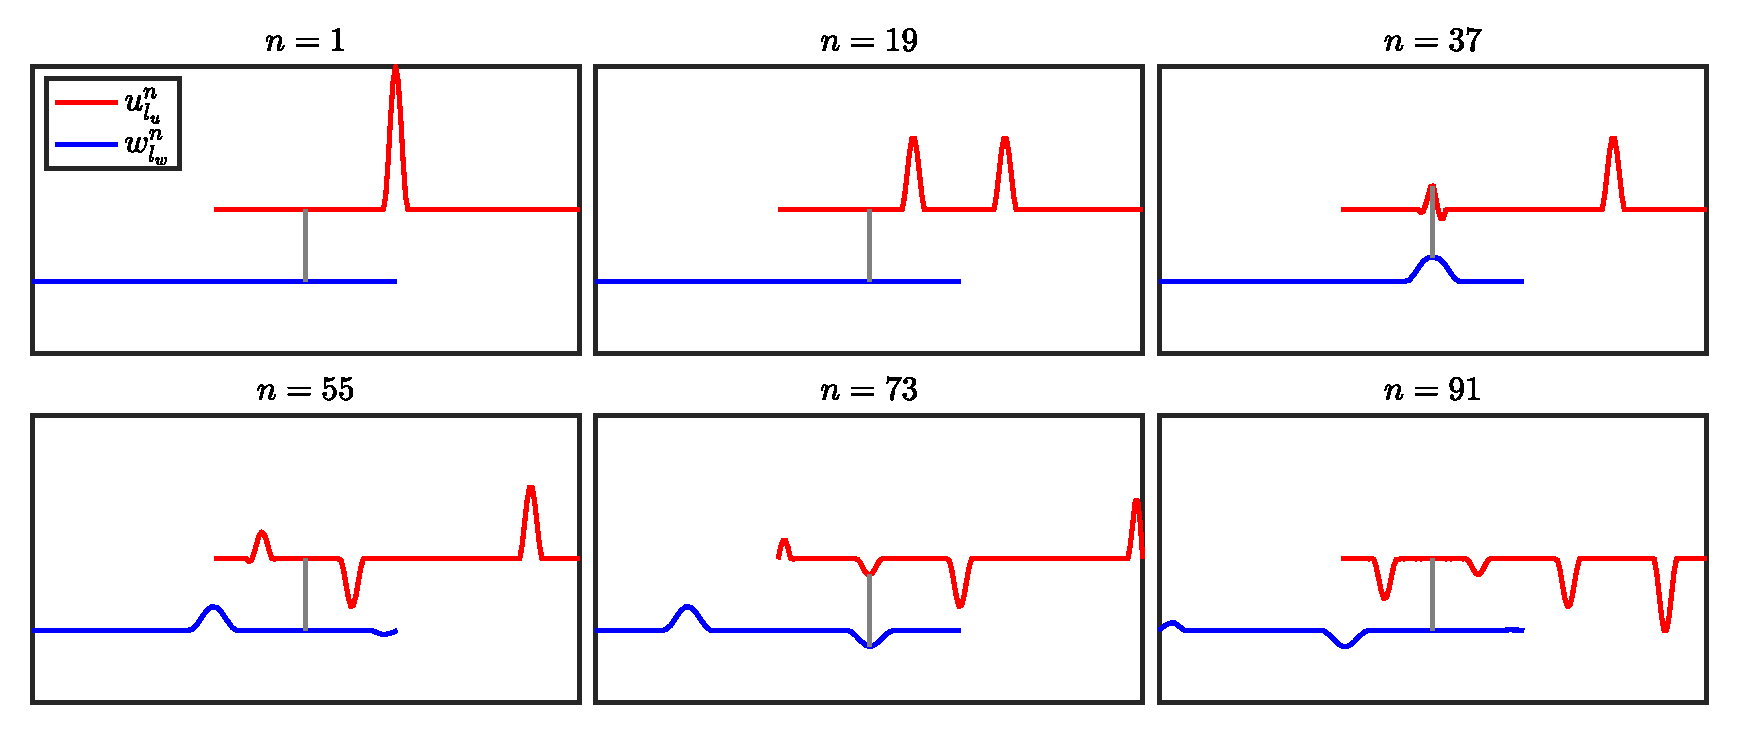
\includegraphics[width=\textwidth]{figures/interactions/connectedWaveEqs.eps}
    \caption{The behaviour of two connected 1D wave equations. The systems are offset for clarity, but the relative displacement at the connection location is 0. \label{fig:connectedWaveEqs}}
\end{figure}

\subsection{Notation simplification}\label{sec:notationSimplification}
In the above equations, the orders of the spreading and interpolation operators have been left unspecified to retain generality. If one would like to connect two systems at specified grid points (so not in-between), the notation can be greatly simplified.%\footnote{The same can be achieved if the orders of the interpolation and spreading operators are chosen to be 0, or if $\alpha_\itxt = 0$ for arbitrary orders.}

Recalling that $\Iu = I_{l, o_u, u}(x_\ctxt)$ and $\Iw = I_{l, o_w, w}(\chi_\ctxt)$, one can set the interpolation orders to 0, i.e., $o_u = o_w = 0$, to yield the following short-hand notations
\begin{equation}\label{eq:shorthandI}
    I_{l,0,u}(x_\text{c})\uln = \ulcn, \qaq I_{m,0,w}(\chi_\text{c})\wmn = \wmcn,
\end{equation}
where $l_\ctxt = \floor[x_\ctxt/h_u]$ and $m_\ctxt = \floor[\chi_\ctxt/h_w]$,
\begin{equation}\label{eq:shorthandJ}
    \lVert J_{l, 0, u}(x_\text{c})\rVert_{d_u}^2 = \frac{1}{h_u} \qaq \lVert J_{m, 0, w}(\chi_\text{c})\rVert_{d_w}^2 = \frac{1}{h_w}.
\end{equation}
This simplifies Eqs. \eqref{eq:conn1DwaveFDSXc} to
\begin{subequations}\label{eq:conn1DwaveFDSXcSimple}
    \begin{align}
        \dtt \ulcn &= c_u^2 \dxx \ulcn -\frac{f^n}{\rho_u A_u h_u}, \label{eq:conn1DwaveuXcSimple} \\
        \dtt \wmcn &= c_w^2 \delta_{\chi\chi} \wmcn + \frac{f^n}{\rho_w A_w h_w},\label{eq:conn1DwavewXcSimple}
    \end{align}
\end{subequations}
which, after rewriting Eq. \eqref{eq:discAccelRigid} to
\begin{equation}
    \dtt\ulcn = \dtt\wmcn,
\end{equation}
one can solve for $f^n$, yielding the following  simplified form of Eq. \eqref{eq:rigidForce}
\begin{equation}
    f^n = \frac{c_u^2 \dxx \ulcn - c_w^2 \delta_{\chi\chi} \wmcn}{\frac{1}{\rho_u A_u h_u} + \frac{1}{\rho_w A_w h_w}}\ .
\end{equation}
Through this simplification, one can now clearly see that the connection forces acting on each respective ideal string in Eq. \eqref{eq:conn1DwaveFDSXcSimple}, are scaled by the mass of one grid `section'  as explained in Section \ref{sec:alternativeInterp}.

\subsection{Energy Analysis}\label{sec:energyAnalysis1DwaveConnRigid}
This section follows the energy analysis techniques shown in Section \ref{sec:energyAnalysis}, though not explicitly following the steps for brevity. As the analysis has previously been performed on the 1D wave equation, this part will not be detailed here. 

Starting with the FD scheme in Eq. \eqref{eq:conn1DwaveFDSu}, one can take an inner product of the scheme (after a multiplication with $\rho_u A_u$) with $(\dtd\uln)$ over discrete domain $d_u$, to get
\begin{equation}\label{eq:powerBalanceConn1DwaveU}
    \dtp \h_u = \langle \dtd\uln, -\Ju f^n\rangle_{d_u},
\end{equation}
where $\h_u$ is the total energy in system $u$ and is as defined in Eq. \eqref{eq:energyBalance1DWave}. The same can be done for Eq. \eqref{eq:conn1DwaveFDSw} (after a multiplication with $\rho_w A_w$) by taking an inner product with $(\dtd\wmn)$ over discrete domain $d_w$ to get 
\begin{equation}\label{eq:powerBalanceConn1DwaveW}
    \dtp \h_w = \langle \dtd\wmn, \Jw f^n\rangle_{d_w},
\end{equation}
where $\h_w$ is the total energy in system $w$. As the total energy in the system is an addition of $\h_u$ and $\h_w$, and using identity \eqref{eq:identityIJ} for the right hand sides of Eqs. \eqref{eq:powerBalanceConn1DwaveU} and \eqref{eq:powerBalanceConn1DwaveW}, one can write 
\begin{equation}\label{eq:rOCconnSystem}
    \dtp (\h_u + \h_w) = -\Iu \dtd \uln f^n + \Iw \dtd \wmn f^n.
\end{equation}
Finally, due to the rigid connection in Eq. \eqref{eq:discRigid}, $\Iu \dtd \uln = \Iw \dtd \wmn$ (if the displacements are equal, their velocities must also be) and the right hand side vanishes:
\begin{equation*}
    \dtp (\h_u + \h_w) = 0.
\end{equation*}
This shows that the rigid connection does not affect the total energy in the system and thus does not affect the stability of the scheme.

Figure \ref{fig:energyConn1DWave} shows the energy of an implementation of the 1D wave system in \eqref{eq:conn1DwaveFDS} corresponding to the behaviour shown in Figure \ref{fig:connectedWaveEqs}. One can observe that energy is transferred from 
\begin{figure}[h]
    \centering
    \begin{tikzpicture}[->,node distance=3cm,
        thick,main node/.style={circle,draw}]
    
        \node[] (image) at (0,0) {
        \includegraphics[width=\textwidth]{figures/interactions/connected1DEnergy.eps}
        };
    
        \node[] (he) at (0.2,0.5) {\small $\mathfrak{h}_\text{e}$};

        \node[] (h) at (-5.9, 1) {\small $\mathfrak{h}$};
        \node[] (v) at (-5.9, 0.5) {\small $\color{red}\mathfrak{h}_u$};
        \node[] (t) at (-5.9, 0) {\small $\color{blue}\mathfrak{h}_w$};
      \end{tikzpicture}
      \caption{The energy of $u$ (red), the energy of $w$ (blue), and the total (black) energy of the system of connected 1D wave equations in \eqref{eq:conn1DwaveFDS}. The energy corresponds to Figure \ref{fig:connectedWaveEqs}. The right panel shows the normalised energy (according to Eq. \eqref{eq:normalisedEnergy}) and shows that the deviation of the energy is within machine precision. \label{fig:energyConn1DWave}}
\end{figure}

\subsection{Matrix form}\label{sec:matrixFormRigid}
% In order to perform a modal analysis on the system, one must use the matrix form of the system in Eq. \eqref{eq:conn1DwaveMatrix}. 

One can write the system in Eq. \eqref{eq:conn1DwaveFDS} with a rigid connection in matrix form, albeit slightly more involved due to the interconnection of the schemes.

To start, the definition of the force in Eq. \eqref{eq:rigidForce} must be substituted into the system, which, after expansion of the left hand side of the system, becomes
\begin{subequations}\label{eq:forceExpanded1Dwaves}
    \begin{align}
        &\begin{aligned}
            u_l^{n+1} &= 2\uln - u_l^{n-1} + c^2k^2\dxx \uln \\
            &- \Ju\frac{k^2}{\rho_u A_u} \left(\frac{c_u^2 \Iu\dxx \uln - c_w^2 \Iw\delta_{\chi\chi} \wmn}{\frac{\lVert \Ju\rVert_{d_u}^2}{\rho_u A_u} + \frac{\lVert \Jw\rVert_{d_w}^2}{\rho_w A_w}}\right), 
        \end{aligned}\\
        &\begin{aligned}
            w_m^{n+1} &= 2\wmn - w_m^{n-1} + c^2k^2\dxx \wmn \\
            &+ \Jw\frac{k^2}{\rho_w A_w} \left(\frac{c_u^2 \Iu\dxx \uln - c_w^2 \Iw\delta_{\chi\chi} \wmn}{\frac{\lVert \Ju\rVert_{d_u}^2}{\rho_u A_u} + \frac{\lVert \Jw\rVert_{d_w}^2}{\rho_w A_w}}\right).
        \end{aligned}
    \end{align}
\end{subequations}
Using Dirichlet boundary conditions for both ideal strings, their values can be stored in the following vectors:
\begin{equation*}
    \u^n =[u_1^n, \hdots, u_{N_u-1}^n]^T, \qaq \w^n =[w_1^n, \hdots, w_{N_u-1}^n]^T.
\end{equation*}
These vectors can then be concatenated to one larger state vector, and after the terms in Eqs. \eqref{eq:forceExpanded1Dwaves} are grouped by the grid functions at various time indices, one obtains the following compact matrix form of system \eqref{eq:conn1DwaveFDS}:
\begin{equation}\label{eq:conn1DwaveMatrix} 
    \begin{bmatrix}
        \u^{n+1}\\
        \w^{n+1}
    \end{bmatrix} = \B \begin{bmatrix}
        \u^n\\
        \w^n
    \end{bmatrix} - \begin{bmatrix}
        \u^{n-1}\\
        \w^{n-1}
    \end{bmatrix},
\end{equation}
% \begin{equation}
%     \mathbf{v}^{n+1} = \B \mathbf{v}^n - \mathbf{v}^{n-1}
% \end{equation}
where 
\begin{equation*}
    \B = \begin{bmatrix}
        \B_u & \mathbf{0}\\
        \mathbf{0} & \B_w 
    \end{bmatrix} + \begin{bmatrix}
        -\j_u\\
        \j_w
    \end{bmatrix}
    \begin{bmatrix}
        \mathbf{f}_u& -\mathbf{f}_w
    \end{bmatrix}.
\end{equation*}
The matrix in the definition of $\B$ contains the operations of the 1D wave equation (also see Eq. \eqref{eq:1DwaveMatrix}),
\begin{equation}    
    \B_u = 2\I_{N_u-1} +c_u^2k^2 (\Dxx)_u, \qaq \B_w = 2\I_{N_w-1} +c_w^2k^2 (\Dxx)_w,
\end{equation}
where matrices $(\Dxx)_u$ and $(\Dxx)_w$ are as defined in Eq. \eqref{eq:DxxDef} and are of the appropriate sizes. The vector multiplication in the definition of $\B$ results in a matrix, and adds the effect of the connection force to the system. Here, $\j_u$ and $\j_w$ are column vectors of size $(N_u-1)\times 1$ and $(N_w-1)\times 1$ containing the values of the spreading operators $\Ju$ and $\Jw$ respectively. Finally,
\begin{equation*}
    \mathbf{f}_u = \frac{k^2}{\rho_uA_u} \left(\frac{c_u^2\i_u(\Dxx)_u}{\frac{\i_u \j_u}{ \rho_u A_u} + \frac{\i_w \j_w}{\rho_w A_w}}\right), \qaq \mathbf{f}_w =  \frac{k^2}{\rho_wA_w}\left(\frac{c_w^2 \i_w(\Dxx)_w}{\frac{\i_u \j_u}{ \rho_u A_u} + \frac{\i_w \j_w}{\rho_w A_w}}\right),
\end{equation*}
%are row vectors of size $1\times (N_u-1)$ and $1\times (N_w-1)$, 
where $\i_u$ and $\i_w$ are row vectors of size $1\times (N_u-1)$ and $1\times (N_w-1)$ containing the values of the interpolation operators $\Iu$ and $\Iw$ respectively. Here, $\i_u\j_u$ and $\i_w\j_w$ are matrix-vector forms of $\lVert \Ju\rVert_d^2$ and $\lVert \Jw\rVert_d^2$ respectively (see Eq. \eqref{eq:JnormIJ}) and reduce to a scalar.

Equation \eqref{eq:conn1DwaveMatrix} can then easily be rewritten in one-step form as described in Section \ref{sec:oneStepForm} and used for modal analysis.\footnote{As the system does not exhibit damping, it could be analysed directly, not using a one-step form.}
% Following Section \ref{sec:oneStepForm}, one can rewrite Eq. \eqref{eq:conn1DwaveMatrix} to

% \begin{equation}
%     \underbrace{\begin{bmatrix}
%         \u^{n+1}\\
%         \w^{n+1}\\
%         \u^{n}\\
%         \w^{n}
%     \end{bmatrix}}_{\mathbf{v}^{n+1}} = \underbrace{\begin{bmatrix}
%         \B & -\I\\
%         \I,& \mathbf{0}
%     \end{bmatrix}}_{\Q}\underbrace{\begin{bmatrix}
%         \u^{n}\\
%         \w^{n}\\
%         \u^{n-1}\\
%         \w^{n-1}
%     \end{bmatrix}}_{\mathbf{v}^n},
% \end{equation}
% one can insert a test solution $\mathbf{v}^n=z^n\boldPhi$ to get
% \begin{equation*}
%     z\boldPhi = \Q\boldPhi,
% \end{equation*}
% and solved for the $p$\th eigenvalue by following the process in Section \ref{sec:oneStepForm}.

% \todo{figure?}

\section{Spring connection}\label{sec:springConnection}
An alternative connection type is the \textit{spring connection}. As in the rigid case, forces are still equal and opposite, but spring connections allow the relative displacement between the two connected elements to be non-zero. This relative displacement is used to determine the connection force. Interestingly, a nonlinear component can be added to this connection without making the system implicit. The most complex springs used in this project have a linear and a nonlinear (cubic) component, as well as a damping term. For ease of explanation, this section will only use a linear spring. A damped nonlinear spring will appear in Section \ref{sec:stringPlateConnection}. 

The force between two components connected by a linear spring can be defined as
\begin{equation}\label{eq:linearSpringForceCont}
    f = f(t) = K\eta,
\end{equation}
where $K\geq 0$ is the spring constant (in N/m) and
\begin{equation}\label{eq:etaLinSpringCont}
    \eta = \eta(t) = u(x_\ctxt, t) - w(\chi_\ctxt, t)
\end{equation}
is the relative displacement between the two systems at their respective connection locations (in m).\footnote{Note that if $u$ was placed 'below' $w$ (see Section \ref{sec:connIdealStrings}), the signs of the force terms in system \eqref{eq:conn1DwaveFDS} would have been flipped and $u(x_\ctxt, t)$ would have been subtracted from $w(\chi_\ctxt, t)$ in Eq. \eqref{eq:etaLinSpringCont} instead.} 

% This is important for the signs when adding the force terms to the schemes.
%$\eta$ is thus also, effectively, the length of the spring.

In discrete time, Eq. \eqref{eq:linearSpringForceCont} becomes
\begin{equation}\label{eq:linearSpringForceDisc}
    f^n = K\mtd\eta^n,
\end{equation}
where
\begin{equation}\label{eq:discEtaConn1Dwave}
    \eta^n = \Iu\uln - \Iw\wmn.
\end{equation}
Here, the centred averaging operator is used for stability (see Section \ref{sec:conn1DwaveEnergySpring}), but when substituted into system \eqref{eq:conn1DwaveFDSXc} seems to make the system implicit. However, one can find an explicit solution, even for an arbitrary amount of connections \cite{Bilbao2009Modular}. These systems are therefore referred to as being \textit{semi-implicit}, and the process of how to solve the system explicitly will be shown below.

\subsection{Explicit solution}\label{sec:explicitSolutionSpringConn}
Compared to the rigid connection in Section \ref{sec:rigidConn}, solving for $f^n$ requires an extra step. After isolating the schemes at their respective connection locations -- resulting in Eqs. \eqref{eq:conn1DwaveFDSXc} -- one needs to expand the scheme and solve for the states at $n+1$:
\begin{subequations}\label{eq:intermediateConn1Dwave}
    \begin{align}
        \Iu u_l^{n+1} &= u^\star - \lVert\Ju\rVert_{d_u}^2 \frac{k^2f^n}{\rho_u A_u},\\
        \Iw w_m^{n+1} &= w^\star + \lVert\Jw\rVert_{d_w}^2 \frac{k^2f^n}{\rho_w A_w},
    \end{align}
\end{subequations}
where
\begin{equation*}
    u^\star = \Iu(2\uln - u_l^{n-1}) + c_u^2k^2\Iu\dxx\uln,
\end{equation*}
and
\begin{equation*}
    w^\star = \Iw(2\wmn - w_m^{n-1}) + c_w^2k^2\Iw\dxx\wmn,
\end{equation*}
are the update equations of the system at their respective connection locations, without the term containing the connection force (as done in Chapter \ref{ch:collisions}). Evaluating Eq. \eqref{eq:discEtaConn1Dwave} at $n+1$ yields
\begin{equation*}
    \eta^{n+1} = \Iu u_l^{n+1} - \Iw w_m^{n+1},
\end{equation*}
into which Eqs. \eqref{eq:intermediateConn1Dwave} can be substituted, as
\begin{equation}\label{eq:etaNp1Schemes}
    \eta^{n+1} = u^\star - \lVert\Ju\rVert_{d_u}^2 \frac{k^2f^n}{\rho_u A_u} - \left(w^\star + \lVert\Jw\rVert_{d_w}^2 \frac{k^2f^n}{\rho_w A_w}\right).
\end{equation}
A second definition for $\eta^{n+1}$ can be obtained after expanding Eq. \eqref{eq:linearSpringForceDisc}:
\begin{equation}\label{eq:etaExpanded}
    \eta^{n+1} = \frac{2 f^n}{K} - \eta^{n-1}
\end{equation}
and can be substituted into Eq. \eqref{eq:etaNp1Schemes} to get
\begin{equation}
    \frac{2 f^n}{K} - \eta^{n-1} = u^\star - \lVert\Ju\rVert_{d_u}^2 \frac{k^2f^n}{\rho_u A_u} - \left(w^\star + \lVert\Jw\rVert_{d_w}^2 \frac{k^2f^n}{\rho_w A_w}\right).
\end{equation}
Finally, one can group the terms for $f^n$ 
\begin{equation*}
    \left(\frac{2}{K} + \frac{\lVert\Ju\rVert_{d_u}^2k^2}{\rho_u A_u} +  \frac{\lVert\Jw\rVert_{d_w}^2k^2}{\rho_w A_w}\right)f^n = u^\star - w^\star + \eta^{n-1}
\end{equation*}
and solve for the force, solely based on known values of the system
\begin{equation}
    f^n = \frac{u^\star - w^\star + \eta^{n-1}}{\frac{2}{K} + \frac{\lVert\Ju\rVert_{d_u}^2k^2}{\rho_u A_u} +  \frac{\lVert\Jw\rVert_{d_w}^2k^2}{\rho_w A_w}}\ .
\end{equation}

Figure \ref{fig:connectedWaveEqsSpring} shows the behaviour of system Eq. \eqref{eq:conn1DwaveFDS}, connected with a spring with spring constant $K = 5\cdot 10^4$ N/m. The same parameters, excitation and connection locations are used as for the rigid connection in Section \ref{sec:rigidConn}. Compared to the behaviour of the system with a rigid connection in Figure \ref{fig:connectedWaveEqs}, one can observe that the distance between the two connected points gets larger as the wave passes the connection point, which corresponds to the extension of the spring. 
% Furthermore, the transfer of energy from $u$ to $w$ is slower than in the rigid case due to the spring extension (see \ref{sec:energy.

\begin{figure}[h]
    \centering
    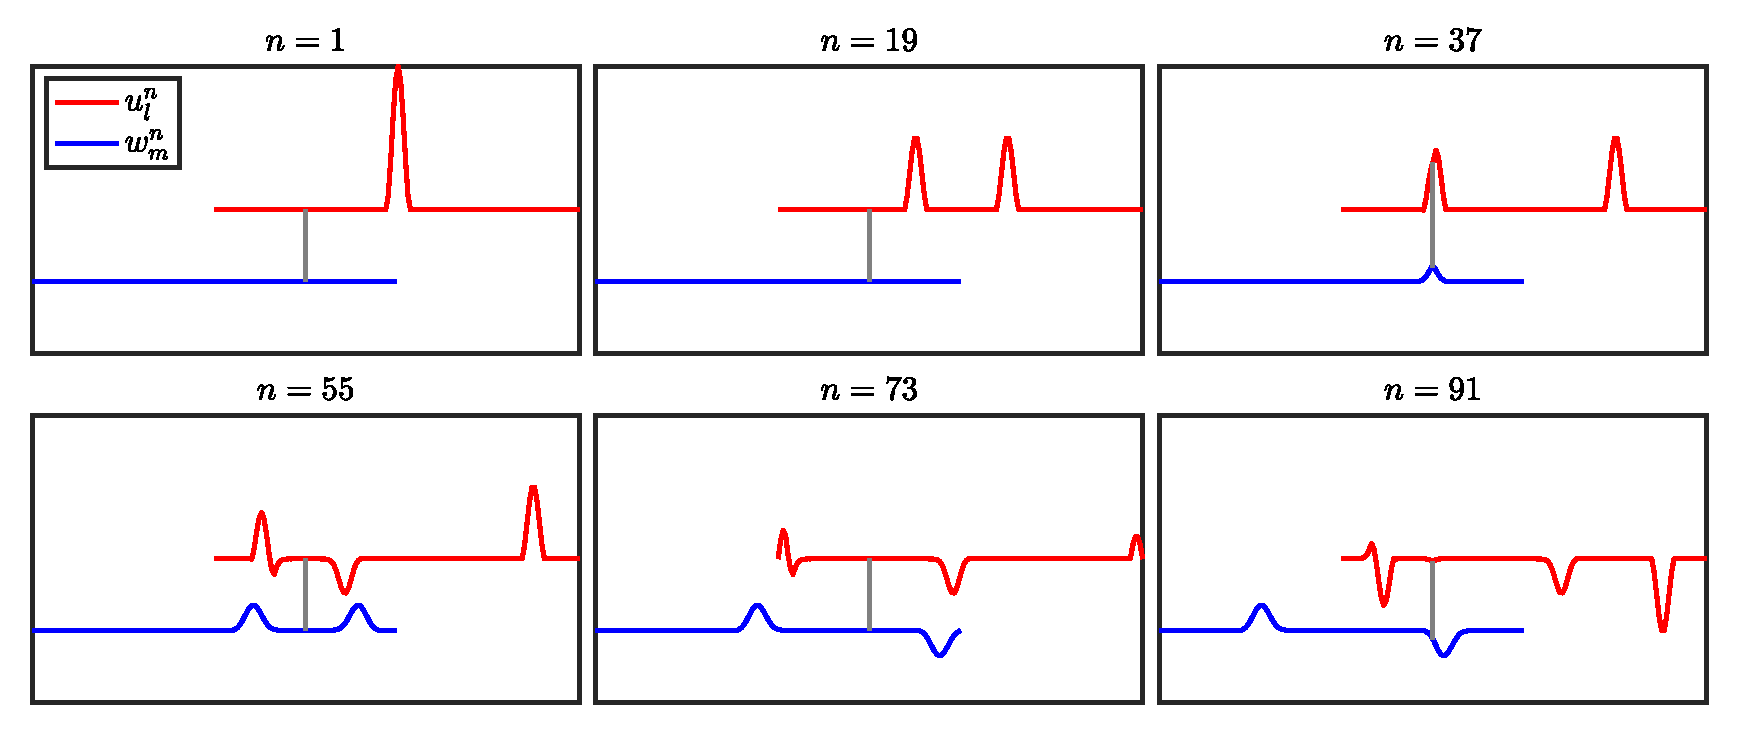
\includegraphics[width=\textwidth]{figures/interactions/connectedWaveEqsSpring.eps}
    \caption{The behaviour of two ideal strings connected using a spring. The systems are offset for clarity, but the relative displacement at the connection location at the start of the simulation is 0. \label{fig:connectedWaveEqsSpring}}
\end{figure}

\subsection{Energy analysis}\label{sec:conn1DwaveEnergySpring}
% As springs store energy themselves, it needs to be shown that stability is maintained.\todo{wording} 
This section follows the energy analysis techniques presented in Section \ref{sec:energyAnalysis} (without explicitly following the steps for brevity) and shows that the discretisation of the spring force chosen in Eq. \eqref{eq:linearSpringForceDisc} is inherently stable. 

Following the same process as in Section \ref{sec:energyAnalysis1DwaveConnRigid}, one can analyse system \eqref{eq:conn1DwaveFDS}, and arrive at Eq. \eqref{eq:rOCconnSystem}:
\begin{equation*}
    \dtp (\h_u + \h_w) = -\Iu \dtd \uln f^n + \Iw \dtd \wmn f^n,
\end{equation*}
which can be rewritten to
\begin{equation*}
    \dtp (\h_u + \h_w) = -\dtd\left(\Iu \uln - \Iw \wmn\right)f^n.
\end{equation*}
One can then substitute the definitions for $f^n$ and $\eta^n$ from Eqs. \eqref{eq:linearSpringForceDisc} and \eqref{eq:discEtaConn1Dwave} to get
\begin{equation}\label{eq:energyAfterForceSubstitution}
    \dtp (\h_u + \h_w) = -K(\dtd \eta^n) (\mtd \eta^n),
\end{equation}
which, using identity \eqref{eq:prodIdentity4}, can be rewritten to
\begin{equation}
    \dtp (\h_u + \h_w + \h_\ctxt) = 0,
\end{equation}
where
\begin{equation}
    \h_\ctxt = \frac{K}{2}\left(\mtm(\eta^n)^2\right)
\end{equation}
is the energy stored by the connection. As this definition is non-negative it does not affect the stability of the system. The spring constant $K$ could potentially be infinitely large, which would effectively reduce the spring connection to a rigid connection presented in Section \ref{sec:rigidConn}.

Figure \ref{fig:energyConn1DWaveSpring} shows the energy of an implementation of system \eqref{eq:conn1DwaveFDS} connected with a spring with spring constant $K=5\cdot 10^4$. other parameters are the same as for the rigid connection in Section \ref{sec:rigidConn}. One can observe that when compared to Figure \ref{fig:energyConn1DWave}, less energy is transferred from $u$ to $w$, and some energy is stored in the spring shown in green. 


\begin{figure}[h]
    \centering
    \begin{tikzpicture}[->,node distance=3cm,
        thick,main node/.style={circle,draw}]
    
        \node[] (image) at (0,0) {
        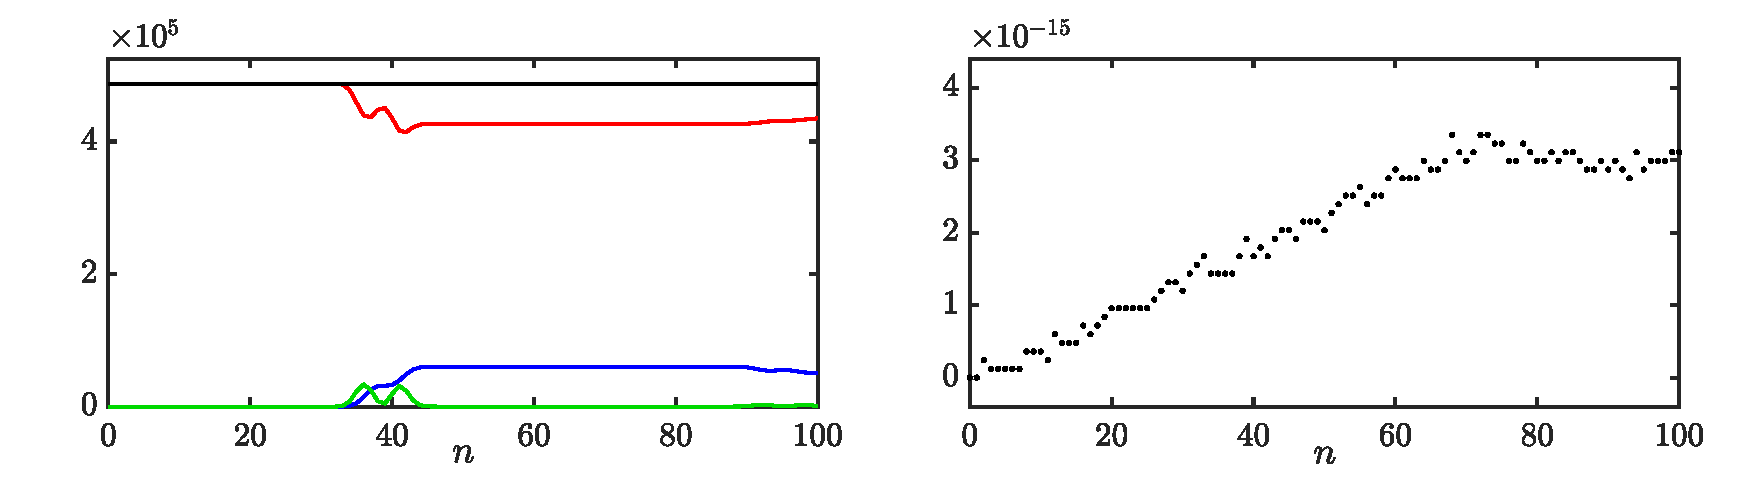
\includegraphics[width=\textwidth]{figures/interactions/connected1DEnergySpring.eps}
        };
    
        \node[] (he) at (0.2,0.5) {\small $\mathfrak{h}_\text{e}$};

        \node[] (h) at (-5.8, 1) {\small $\mathfrak{h}$};
        \node[] (v) at (-5.8, 0.5) {\small $\color{red}\mathfrak{h}_u$};
        \node[] (t) at (-5.8, 0) {\small $\color{blue}\mathfrak{h}_w$};
        \node[] (c) at (-5.8, -0.5) {\small $\color[HTML]{00DB00}\mathfrak{h}_\ctxt$};

      \end{tikzpicture}
      \caption{The energy of $u$ (red), the energy of $w$ (blue), the energy of the spring connection (green) and the total energy (black) of the system of connected 1D wave equations in \eqref{eq:conn1DwaveFDS}. The energy corresponds to the system in Figure \ref{fig:connectedWaveEqsSpring}. The right panel shows the normalised energy (according to Eq. \eqref{eq:normalisedEnergy}) and shows that the deviation of the energy is within machine precision. \label{fig:energyConn1DWaveSpring}}
\end{figure}

\subsubsection{Unstable discretisation}
To show why an averaging operator is used in Eq. \eqref{eq:linearSpringForceDisc}, consider a more straightforward discretisation of Eq. \eqref{eq:linearSpringForceCont} without the averaging operator, such that
\begin{equation*}
    f^n = K\eta^n.
\end{equation*}
Performing an energy analysis of the system would yield 
\begin{equation*}
    \dtp (\h_u + \h_w) = -K(\dtd \eta^n) (\eta^n),
\end{equation*}
(instead of Eq. \eqref{eq:energyAfterForceSubstitution}) and using identity \eqref{eq:prodIdentity2}, this can be rewritten to
\begin{equation*}
    \dtp (\h_u + \h_w + \h_\ctxt) = 0,
\end{equation*}
where
\begin{equation*}
    \h_\ctxt = \frac{K}{2}\left(\eta^ne_{t-}\eta^n\right).
\end{equation*}
As this is not necessarily non-negative, the connection places a larger restriction on the stability of the system at the connection location. In other words, $\lambda \leq 1$ for the ideal strings does not ensure stability at the connection location. Also see \cite[pp. 190--192]{theBible}.

% \section{Spring-like connections}

% Forces are still equal and opposite as the springs are not distributed...

% \subsection{Connection with rigid barrier (scaled)}
% Consider the (scaled) 1D wave equation with an additional force term $F^n$
% \begin{equation}\label{eq:1DwaveConnRigid}
%     \dtt \uln = \gamma^2\dxx \uln + J_l(x_\ctxt)F^n
% \end{equation}
% where
% \begin{equation}\label{eq:1DwaveConnRigidForce}
%     F^n = -\omega_0^2\mtd\eta^n - \omega_1^4(\eta^n)^2\mtd\eta^n - 2\sigma_\times \dtd \eta^n
% \end{equation}
% and
% \begin{equation}\label{eq:etaRigid}
%     \eta^n = I_l(x_\ctxt)\uln.
% \end{equation}

% To obtain $F^n$, an inner product of scheme \eqref{eq:1DwaveConnRigid} needs to be taken with $J_l(x_\ctxt)$ over domain $\D$ which, using identity \eqref{eq:identityIJ} yields 
% \begin{equation}\label{eq:1DwaveConnRigidInnerProd}
%     \dtt I_l(x_\ctxt)\uln = \gamma^2 I_l(x_\ctxt)\dxx \uln + \underbrace{I_l(x_\ctxt)J_l(x_\ctxt)}_{\lVert J_l(x_\ctxt) \rVert^2_\D}F^n.
% \end{equation}
% As $u$ is connected to a rigid barrier according to \eqref{eq:etaRigid}, a shortcut can be taken and Eqs. \eqref{eq:1DwaveConnRigidForce} and \eqref{eq:etaRigid} can be directly substituted into Eq. \eqref{eq:1DwaveConnRigidInnerProd} to get
% \begin{equation}
%     \dtt \eta^n = \gamma^2 I_l(x_\ctxt)\dxx \uln + \lVert J_l(x_\ctxt)\rVert^2_\D\left( -\omega_0^2\mtd\eta^n - \omega_1^4(\eta^n)^2\mtd\eta^n - 2\sigma_\times \dtd \eta^n\right).
% \end{equation}
% and solved for $\eta^{n+1}$:
% \begin{equation}
%     \begin{aligned}
%     &\!\!\!\!\!\!\!\!\!\!\!\!\!\!\Big(1 + \lVert J_l(x_\ctxt)\rVert^2_\D k^2[\omega_0^2/2 + \omega_1^4(\eta^n)^2/2 + \sigma_\times/k] \Big)\eta^{n+1} \\
%    = &\ 2 \eta^n - \Big(1 + \lVert J_l(x_\ctxt)\rVert^2_\D k^2[\omega_0^2/2 + \omega_1^4(\eta^n)^2/2 - \sigma_\times/k]\Big)
%     \eta^{n-1}\\
%     &+ \gamma^2k^2 I_l(x_\ctxt)\dxx\uln
%     \end{aligned}
% \end{equation}
% This can then be used to calculate $F^n$ in \eqref{eq:1DwaveConnRigidForce} and can in turn be used to calculate $u_l^{n+1}$ in \eqref{eq:1DwaveConnRigid}.

\section{String-plate connection}\label{sec:stringPlateConnection}
As an example of a more complicated connected system used in papers \citeP[A] and \citeP[B], consider a stiff string connected to a plate using a nonlinear damped spring. This could be interpreted as a simplified form of how the string would be connected to the body in a stringed instrument. In the following, subscripts `s' and `p' are used to denote a string or plate parameter respectively. 

\subsection{Continuous time}
Consider a damped stiff string of length $L$ (in m), its transverse displacement described by $u = u(\chi,t)$ (in m) defined for $t\geq 0$ and $\chi \in \D_\stxt$ where domain $\D_\stxt = [0, L]$. Its PDE is described by
\begin{equation}
    \rho_\stxt A\ptt u = T \partial_{\chi}^2 u - E_\stxt I \partial_{\chi}^4 u - 2\szX[\stxt]\rho_\stxt A\pt u + 2\soX[\stxt]\rho_\stxt A\pt\partial_{\chi}^2 u,
\end{equation}
where parameters are as in Eq. \eqref{eq:stiffStringPDE}.

The transverse displacement of a damped rectangular thin plate of side lengths $L_x$ and $L_y$ (both in m) can be described as $w=w(x,y,t)$ (in m), which is defined for $t\geq 0$ and $(x,y)\in \D_p$ where domain $\D_p = [0, L_x] \times [0, L_y]$. Its PDE is defined as
\begin{equation}
    \rho_\ptxt H\ptt w = -D\Delta\Delta w - 2\szX[\ptxt]\rho_\ptxt H\pt w + 2\soX[\ptxt] \rho_\ptxt H\pt\pxx w,
\end{equation}
where parameters are as in Eq. \eqref{eq:platePDE}.

One can connect the above PDEs, by adding a localised connection force. After a division by $\rho_\stxt A$ and $\rho_\ptxt H$ respectively the connected string-plate system becomes
\begin{subequations}\label{eq:connStringPlatePDEs}
    \begin{align}
        \ptt u &= c^2 \partial_{\chi}^2 u - \kappa_\stxt^2 \partial_{\chi}^4 u - 2\szX[\stxt]\pt u + 2\soX[\stxt] \pt\partial_{\chi}^2 u - \delta(\chi-\chi_\ctxt)\frac{f}{\rho_\stxt A},\\
    \ptt w &= -\kappa_\ptxt^2\Delta\Delta w - 2\szX[\ptxt]\pt w + 2\soX[\ptxt] \pt\pxx w + \delta(x-x_\ctxt, y-y_\ctxt)\frac{f}{ \rho_\ptxt H},
    \end{align}
\end{subequations}
where $\delta(\chi-\chi_\ctxt)$ (in m$^{-1}$) and $\delta(x-x_\ctxt, y-y_\ctxt)$ (in m$^{-2}$) are the 1D and 2D spatial Dirac delta functions defined in Eqs. \eqref{eq:spatialDirac} and \eqref{eq:spatialDirac2D} respectively and locate the connection force at $\chi_\ctxt \in \D_s$ (in m) along the string and $(x_\ctxt,y_\ctxt)\in \D_p$ (in $(\text{m}, \text{m})$) on the plate.

The force between the two components (in N) is set to be a nonlinear (cubic) damped spring defined as (used in e.g. \cite{Webb2015} and in scaled form in \cite{Bilbao2009Modular})
\begin{equation}\label{eq:nonlinearForce}
    f = f(t) = K_1\eta+K_3\eta^3+R \dot\eta,
\end{equation}
with linear and nonlinear spring coefficients $K_1$ (in N/m) and $K_3$ (in N/m$^3$) and damping coefficient $R$ (in kg/s). Furthermore, the distance (in m) between the string and the plate at their respective connection locations is defined as
\begin{equation}
    \eta = \eta(t) = u(\chi_\ctxt, t) - w(x_\ctxt, y_\ctxt, t).
\end{equation}


\subsection{Discrete time}
To discretise $u(\chi, t)$, one can use grid function $\uqn$ where $n\in\mathbb{N}^0$ and $q\in\{0, \hdots, N\}$ with number of grid points $N+1$ (see Section \ref{sec:gridFunctions}). Next, $w(x, y, t)$ can be discretised using grid function $\wlmn$ with $l \in \{0, \hdots, N_x\}$ and $m \in \{0, \hdots, N_y\}$ where $N_x+1$ and $N_y+1$ are the number of grid points in the $x$ and $y$ direction respectively (see Section \ref{sec:2Dintro}). 

Using these grid functions, system \eqref{eq:connStringPlatePDEs} can then be discretised as
\begin{align}\label{eq:connStringPlateFDSs}
    &\begin{aligned}
        \dtt \uqn &= c^2 \dcc \uqn - \kappa_\stxt^2 \dcccc \uqn - 2\szX[\stxt]\dtd \uqn + 2\soX[\stxt] \dtm\dcc \uqn \\
        &\qquad - J_q(\chi_\ctxt)\frac{f^n}{\rho_\stxt A}\ ,
    \end{aligned}\\
    &\begin{aligned}
        \dtt \wlmn &= -\kappa_\ptxt^2\dDelta\dDelta \wlmn - 2\szX[\ptxt]\dtd \wlmn + 2\soX[\ptxt] \dtm\dxx \wlmn \\
        &\qquad + J_{l, m}(x_\ctxt, y_\ctxt)\frac{f^n}{\rho_\ptxt H}\ ,
    \end{aligned}
\end{align}
where $J_q(\chi_\ctxt) = J_{q, o_\stxt} (\chi_\ctxt)$ is a 1D spreading operator of order $o_\stxt$ as defined in Section \ref{sec:interpolationSpreading} and $J_{l, m}(x_\ctxt, y_\ctxt) = J_{(l, m), o_\ptxt}(x_\ctxt, y_\ctxt)$ is a 2D spreading operator of order $o_\ptxt$ as defined in Section \ref{sec:interpolationSpreading2D}. 

The definition of the force in Eq. \eqref{eq:nonlinearForce} can be discretised as\footnote{The second-order averaging operator has been chosen here to show an alternative discretisation of the linear term, but it could be replaced by a centred first-order averaging operator as used in Eq. \eqref{eq:linearSpringForceDisc}.}
\begin{equation}\label{eq:discForceStringPlate}
    f^n = K_1\mtt\eta^n+K_3(\eta^n)^2\mtd\eta^n+R\dtd\eta^n,
\end{equation}
where
\begin{equation}\label{eq:discEtaStringPlate}
    \eta^n = I_q(x_\ctxt)\uqn - I_{l, m}(x_\ctxt, y_\ctxt)\wmn.
\end{equation}
Here, $I_q(\chi_\ctxt) = I_{q, o_\stxt} (\chi_\ctxt)$ and $I_{l, m}(x_\ctxt, y_\ctxt) = I_{(l, m), o_\ptxt}(x_\ctxt, y_\ctxt)$ are interpolation operators of the same order as $J_q(\chi_\ctxt)$ and $J_{l,m}(x_\ctxt)$ respectively. 


\subsection{Solving for $f$}
Following the same process as in Section \ref{sec:explicitSolutionSpringConn}, system \eqref{eq:connStringPlateFDSs} needs to be isolated at the connection locations. This is done by taking an inner product of the schemes in \eqref{eq:connStringPlateFDSs} with their respective spreading operators over discrete domains $d_u = \{0, \hdots, N\}$ and $d_w = \{0, \hdots, N_x\}\times \{0, \hdots, N_y\}$ respectively. Taking these inner products, expanding the $\dtt$ and $\dtd$ operators (as these contain $u_q^{n+1}$) and solving for the states at $n+1$ yields
\begin{subequations}\label{eq:connStringPlateFDSsAtConn}
    \begin{align}
        \Iq u_q^{n+1} &= u^\star- \lVert J_q(\chi_\ctxt)\rVert_{d_u}^2\frac{k^2f^n}{\rho_\stxt A(1+\szX[\stxt]k)}\ ,\\
        \Ilm w_{l,m}^n &= w^\star+ \lVert J_{l, m}(x_\ctxt, y_\ctxt)\rVert_{d_w}^2\frac{k^2f^n}{\rho_\ptxt H(1+\szX[\ptxt]k)}\ ,
    \end{align}
\end{subequations}
where
\begin{subequations}
\begin{align}
    &\begin{aligned}
        u^{\star} =&\ \Big(\Iq (2\uqn - u_q^{n-1}) + c^2k^2 \Iq\dcc \uqn - \kappa_\stxt^2k^2 \Iq\dcccc \uqn\\
        &\quad+ \szX[\stxt]k\Iq u_q^{n-1} + 2\soX[\stxt]k^2 \Iq\dtm\dcc \uqn\Big) / (1+\szX[\stxt]k),
    \end{aligned}\label{eq:stringPlateUStar}\\
    &\begin{aligned}
        w^\star =&\ \Big(-\kappa_\ptxt^2\Ilm\dDelta\dDelta \wlmn + \szX[\ptxt]k\Ilm w_{l,m}^{n-1} \\
        &\qquad\qquad+ 2\soX[\ptxt] \Ilm\dtm\dxx \wlmn\Big)/(1+\szX[\ptxt]k),
    \end{aligned}\label{eq:stringPlateWStar}
\end{align}
\end{subequations}
are the update equations of the schemes at their respective connection locations without the force term. 

Evaluating Eq. \eqref{eq:discEtaStringPlate} at $n+1$ and substituting Eqs. \eqref{eq:connStringPlateFDSsAtConn} yields
\begin{equation}\label{eq:etaNextStringPlate1}
    \begin{aligned}
    \eta^{n+1} =&\ u^\star- \lVert J_q(\chi_\ctxt)\rVert_{d_u}^2\frac{k^2f^n}{\rho_\stxt A(1+\szX[\stxt]k)} \\
    &- \left(w^\star + \lVert J_{l, m}(x_\ctxt, y_\ctxt)\rVert_{d_w}^2\frac{k^2f^n}{\rho_\ptxt H(1+\szX[\ptxt]k)}\right).
    \end{aligned}
\end{equation}
Then expanding Eq. \eqref{eq:discForceStringPlate} to
\begin{equation*}
     f^n = \underbrace{\left(\frac{K_1}{4}+\frac{K_3(\eta^n)^2}{2} + \frac{R}{2k}\right)}_{r_+^n}\eta^{n+1} + \frac{K_1}{2}\eta^n + \underbrace{\left(\frac{K_1}{4}+\frac{K_3(\eta^n)^2}{2} - \frac{R}{2k}\right)}_{r_-^n}\eta^{n-1},
\end{equation*}
and solving for $\eta^{n+1}$ yields
\begin{equation}
    \eta^{n+1} = \frac{f^n}{r_+^n} - \frac{K_1}{2r_+^n}\eta^n - \frac{r_-^n}{r_+^n}\eta^{n-1}.
\end{equation}
Substituting this into Eq. \eqref{eq:etaNextStringPlate1}, one can find a definition for the connecting force
\begin{equation}\label{eq:stringPlateForce}
    f^n = \frac{u^\star - w^\star + \frac{K_1}{2r_+^n}\eta^n + \frac{r_-^n}{r_+^n}\eta^{n-1}}{\frac{1}{r_+^n} + \frac{\lVert J_q(\chi_\ctxt)\rVert_{d_u}^2k^2}{\rho_\stxt A(1+\szX[\stxt]k)} + \frac{\lVert J_{l, m}(x_\ctxt, y_\ctxt)\rVert_{d_w}^2k^2}{\rho_\ptxt H(1+\szX[\ptxt]k)}}\ .
\end{equation}

\subsection{Implementation}\label{sec:implementationStringPlate}
This section shows an example of an implementation of the string-plate system. The parameters for the stiff string can be found in Table \ref{tab:stiffStringParams} (with $L = 1.5$ m and $T = 555$ N) and for the thin plate in Table \ref{tab:thinPlateParams} (with $H=5\cdot10^{-4}$). Both systems use simply supported boundary conditions. Additional parameters used for the connection are
\begin{equation*}
    K_1 = 10^4\ \,\text{N/m}, \quad K_3 = 10^7\ \,\text{N/m}^3, \qaq R = 10\ \,\text{kg/s}.
\end{equation*}
The \texttt{MATLAB} code of the implementation can be found online \cite{stringPlateGist}.\footnote{Note that in the online code, $L$, $L_x$ and $L_y$ have been halved to reduce computations and avoid crashes on some machines.}  Figure \ref{fig:stringPlate} shows a visualisation of the string plate system excited with a raised cosine. 
\begin{figure}[h]
    \centering
    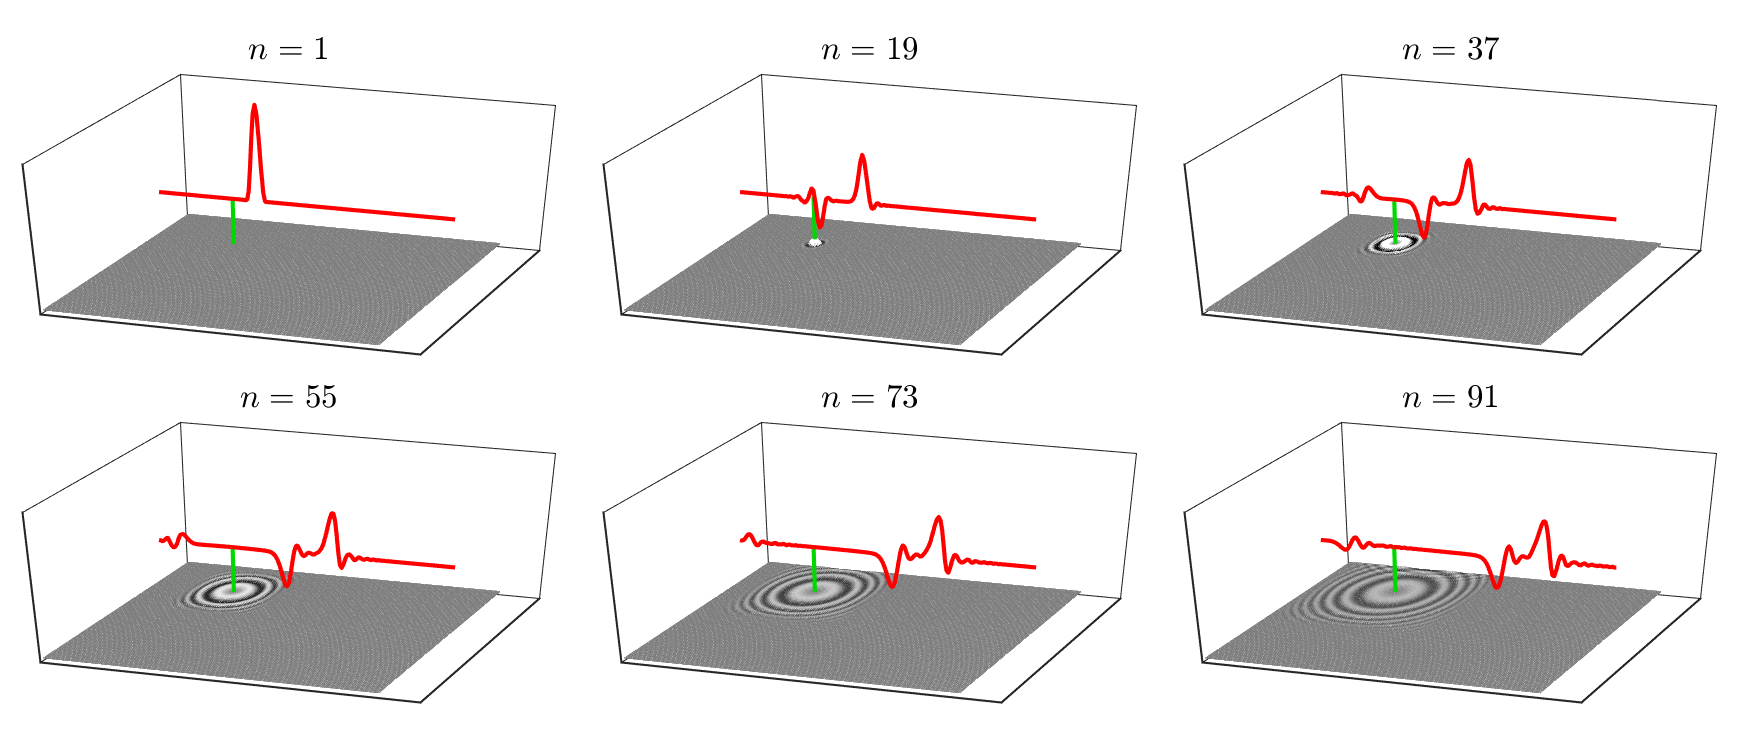
\includegraphics[width=\textwidth]{figures/interactions/stringPlate.eps}
    \caption{The behaviour of the string-plate system connected with a nonlinear damped spring. The string is shown in red, the plate in gray and the connection in green. \label{fig:stringPlate}}
\end{figure}

In the following, the $\i$ and $\j$ vectors are used as in Section \ref{sec:matrixFormRigid} and are of the appropriate sizes. The matrices for the string can be found in Eq. \eqref{eq:matrixFormStiffString} and those for the plate in Eq. \eqref{eq:matrixFormThinPlate}. When implementing connections (or any other interactions for that matter), one mostly performs the following steps in the main loop:
\begin{enumerate}
    \item Calculate the entire scheme without force terms:\\
    \vspace{-0.5em}\begin{equation}\label{eq:stringPlateImp1}
        \u^\star = \frac{\B_\stxt\u^n + \C_\stxt\u^{n-1}}{A_\stxt}, \qaq \w^\star = \frac{\B_\ptxt\w^n + \C_\ptxt\w^{n-1}}{A_\ptxt}\ .
    \end{equation}
    \item Obtain $u^\star$ and $w^\star$:\\
    \vspace{-1em}\begin{equation}\label{eq:stringPlateImp2}
       u^\star = \i_u \u^\star \qaq w^\star = \i_w \w^\star.
    \end{equation}
    \item Calculate the connection force $f^n$ (Eq. \eqref{eq:stringPlateForce}).
    \item Add force terms to the schemes in Eq. \eqref{eq:stringPlateImp1}:\\
    \begin{equation}\label{eq:stringPlateImp4}
        \u^{n+1} = \u^{\star} - \j_u \frac{f^n k^2}{\rho_\stxt A (1+\szX[\stxt])},\qaq \w^{n+1} = \w^{\star} + \j_w \frac{f^n k^2}{\rho_\ptxt H (1+\szX[\ptxt])}.
    \end{equation} 
\end{enumerate}
Calculating $\u^\star$ and $\w^\star$ beforehand reduces computations, and allows $u^\star$ and $w^\star$ to be more easily obtained. 

\subsection{Energy analysis}
Recalling the total energy and damping terms for the string and plate in Sections \ref{sec:energyAnalysisString} and \ref{sec:energyAnalysisThinPlate} respectively, one can --  similar to Eq. \eqref{eq:rOCconnSystem} -- arrive at the following:
\begin{equation}
    \dtp(\h_\stxt + \h_\ptxt) + \q_\stxt + \q_\ptxt = -\Iq (\dtd \uqn)f^n +\Ilm(\dtd \wlmn)f^n,
\end{equation}
which can be rewritten to
\begin{equation*}
    \dtp(\h_\stxt + \h_\ptxt) + \q_\stxt + \q_\ptxt = -\dtd \left(\Iq \uqn - \Ilm\wlmn\right)f^n.
\end{equation*}
Substituting the definitions for $f^n$ and $\eta^n$ from Eqs. \eqref{eq:discForceStringPlate} and \eqref{eq:discEtaStringPlate} respectively, yields
\begin{equation*}
    \dtp(\h_\stxt + \h_\ptxt) + \q_\stxt + \q_\ptxt = -(\dtd\eta^n)(K_1\mtt\eta^n+K_3(\eta^n)^2\mtd\eta^n+R\dtd\eta^n).
\end{equation*}
Due to the nonlinear dependency on $\eta^n$ one must isolate $\dtp$ from the cubic term manually, according to
\begin{align*}
    &\ \ K_3(\eta^n)^2(\dtd \eta^n)(\mtd \eta^n)\\
    = &\ \ \frac{K_3(\eta^2)}{2k}(\eta^{n+1} - \eta^{n-1})\frac{1}{2}(\eta^{n+1} + \eta^{n-1})\\
    = &\ \ \frac{K_3(\eta^n)^2}{4k}\left((\eta^{n+1})^2 - (\eta^{n-1})^2\right)\\
    = &\ \ \frac{K_3}{4k}\left((\eta^{n+1}\eta^n)^2 - (\eta^n\eta^{n-1})^2\right)\\
    = &\ \ \dtp\left(\frac{K_3}{4}(\eta^n\eta^{n-1})^2\right).
\end{align*}
% \begin{equation*}
%     (\dtd \eta^n)K_1\mtt\eta^n \quad \xRightarrow{\text{Eq. \eqref{eq:prodIdentity5}}} \quad \frac{K_1}{8}(\eta^n+\eta^{n-1})^2 
% \end{equation*}
Finally, using identity \eqref{eq:prodIdentity5} for the linear term, the following balance follows
\begin{equation}
    \dtp(\h_\stxt + \h_\ptxt + \h_\ctxt) = - \q_\stxt - \q_\ptxt - \q_\ctxt,
\end{equation}
where the energy stored by the spring connection is
\begin{equation*}
    \h_\ctxt = \frac{K_1}{8}(\eta^n+\eta^{n-1})^2 + \frac{K_3}{4}(\eta^n\eta^{n-1})^2,
\end{equation*}
and the damping term of the connection is
\begin{equation*}
    \q_\ctxt = R(\dtd\eta^n)^2.
\end{equation*}
Figure \ref{fig:energyStringPlate} shows the energetic output of the string-plate system corresponding to the behaviour in Figure \ref{fig:stringPlate}. One can observe that energy is transferred from the string to the plate due to the connection. Furthermore, due to the high value for spring-damping $R$, the total energy decreases substantially as the excitation reaches the connection location along the string. 

\begin{figure}[h]
    \centering
    \begin{tikzpicture}[->,node distance=3cm,
        thick,main node/.style={circle,draw}]
    
        \node[] (image) at (0,0) {
        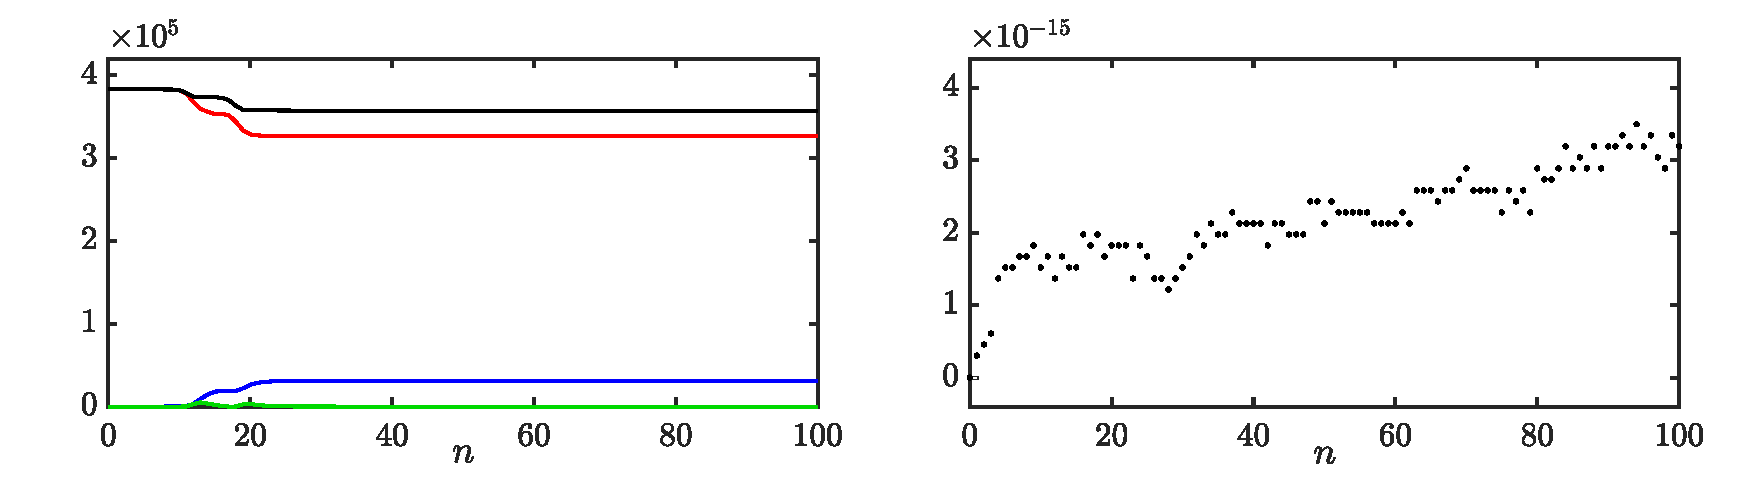
\includegraphics[width=\textwidth]{figures/interactions/stringPlateEnergy.eps}
        };
    
        \node[] (he) at (0.2,0.5) {\small $\mathfrak{h}_\text{e}$};

        \node[] (h) at (-5.8, 1) {\small $\mathfrak{h}$};
        \node[] (v) at (-5.8, 0.5) {\small $\color{red}\mathfrak{h}_\stxt$};
        \node[] (t) at (-5.8, 0) {\small $\color{blue}\mathfrak{h}_\ptxt$};
        \node[] (c) at (-5.8, -0.5) {\small $\color[HTML]{00DB00}\mathfrak{h}_\ctxt$};

      \end{tikzpicture}
      \caption{The energy of the string (red), the plate (blue), the spring connection (green) and the total energy (black) of the connected string-plate system \eqref{eq:connStringPlateFDSs}. The energy corresponds to the system in Figure \ref{fig:stringPlate}. The right panel shows the normalised energy (according to Eq. \eqref{eq:normalisedEnergyDamping}) and shows that the deviation of the energy is within machine precision. \label{fig:energyStringPlate}}
\end{figure}

% \subsection{Non-dimensional}
% The scaled system can be written as:
% \begin{align}
%     \ptt u &= \gamma^2 \pxx u - \kappa_\stxt^2 \pxxxx u - 2\szX[\stxt]\pt u + 2\soX[\stxt] \pt\pxx u - \delta(x-x_\ctxt)F\\
%    \pt w &= -\kappa_\ptxt^2\Delta\Delta w - 2\szX[\ptxt]\pt w + 2\soX[\ptxt] \pt\pxx w + \delta(x-x_\ctxt, y-y_\ctxt)F
% \end{align}
% where
% \begin{equation}
%     F = F(t) = \omega_1^2\eta+\omega_3^4\eta^3+\sigma_\ctxt \dot\eta
% \end{equation}
% and
% \begin{equation}
%     \eta = \eta(t) = u(x_\ctxt, t) - w(x_\ctxt, y_\ctxt, t)
% \end{equation}


% \begin{equation}
%     I(x_\ctxt)\delta_{tt}\uqn = c^2
%     \left(I(x_\ctxt)\dxx\uqn\right) + I(x_\ctxt)J(x_\ctxt)F
% \end{equation}


% \subsubsection{Relative location of objects}\todo{look at this compared to when I talk about it in chapter \ref{ch:collisions}}


% Forces should be equal and opposite. 
\chapter{Collisions}\label{ch:collisions}
Many musical instruments rely on collisions in some shape or form. Examples are the collision between a hammer and a piano string, a guitar pick and the string, and even the collision between the lips of a trumpet player. 

This work uses collision models that rely on penalising methods. The colliding objects -- although possibly perfectly rigid -- are supposed to interpenetrate, and collision is interpreted as a \textit{penalty}. The eventual force acting on the colliding objects is then dependent on the level of penetration. For deformable objects, such as the hammer felt tip of a piano, the penalty is dependent on the level of deformation. These collision models were first used in a musical context by e.g. \cite{Chatziioannou2013, Bilbao2014}.

The discretisations proposed in \cite{Chatziioannou2013, Bilbao2014} rely on implicit nonlinear schemes which require an iterative method, such as the Newton-Raphson method presented in Section \ref{sec:newtonRaphson}, to obtain their solution. 
The exact number of iterations required per time step, especially in interactive applications, is usually unknown. This could be detrimental to real-time applications, as the number of iterations, and consequently the extra number of computations, could be very large in a particular situation. Furthermore, and perhaps more importantly, existence and uniqueness of the solution might not be available. 

In \cite{Ducceschi2021} (co-authored by the PhD student [\hyperref[ch:listOfPublications]{O3}]), Ducceschi et al. propose a method based on quadratisation of the collision potential energy, that circumvents the need of an iterative method to solve nonlinear collisions. Energy quadratisation for explicit schemes first appeared in the context of Port-Hamiltonian systems and was due to Lopes et al. in \cite{Lopes2015}. The introduction of an additional state variable, which is what Ducceschi's work is based on, was introduced in \cite{Yang2017, Jiang2019}. Papers \citeP[D] and \citeP[E] follow an earlier iteration of the non-iterative collision algorithm from \cite{Ducceschi2019, Bilbao2019} which exhibited spurious oscillations that Ducceschi et al. resolve in \cite{Ducceschi2021}. Paper \citeP[H] uses the corrected collision model for the collision between the lips exciting the trombone. The corrected model will be used in this work and presented in this chapter. 

This chapter first provides a definition for the collision potential as well as its quadratisation, used as the basis for the explicit method. Then, the method will be applied to a simple mass-barrier collision and finally, to a mass-spring -- string collision which can be used to model a finger-fretted string.

\subsubsection{Collision potential}
Collisions can be modelled using a nonlinear \textit{collision potential}, which can be defined as
\begin{equation}\label{eq:potential}
    \phi(\eta) = \frac{K_\ctxt}{\alpha_\ctxt+1}[\eta]_+^{\alpha_\ctxt+1},
\end{equation}
with collision stiffness $K_\ctxt \geq 0$ (in N/m$^{\alpha_\ctxt}$) and dimensionless nonlinear collision coefficient $\alpha_\ctxt \geq 1$. Here $\eta = \eta(t)$ describes the relative displacement between the two colliding bodies (in m). The $[\cdot ]_+$ operator, defined as 
\begin{equation}\label{eq:etaPlus}
    [\cdot]_+ = \frac{\cdot + |\cdot|}{2},
\end{equation}
describes the `positive part of' and when applied to $\eta$ in Eq. \eqref{eq:potential} causes the potential $\phi$ to only be non-zero when the two colliding bodies are in contact. 
% See Figure \ref{fig:eta}.
% %
% \begin{figure}[h]
% \centerline{\includegraphics[width=0.6\columnwidth]{figures/interactions/eta.eps}}
% \caption{\label{fig:eta}{A plot of $[\eta]_+$.}}
% \end{figure}

The derivative of Eq. \eqref{eq:potential} with respect to $\eta$ is defined as 
\begin{equation}\label{eq:derivPotential}
    \phi'(\eta) = K_\ctxt[\eta]_+^{\alpha_\ctxt}
\end{equation}
and can then be used in the PDE at hand. 

The issue with this form of the collision potential, is that an iterative method, such as Newton-Raphson presented in Section \ref{sec:newtonRaphson}, needs to be used in order to solve the system \cite{Ducceschi2021}.

\subsubsection{Quadratic form}
In \cite{Ducceschi2021}, the authors propose to rewrite the potential in Eq. \eqref{eq:derivPotential} in a quadratic form. Using the chain rule and  $\psi = \psi(\eta)$, Eq. \eqref{eq:derivPotential} can be rewritten as
\begin{equation}\label{eq:quadraticPotential}
    \phi'(\eta) = \psi\psi' \quad \text{where} \quad \psi = \sqrt{2\phi} \quad \text{and} \quad \psi' = \frac{\dot{\psi}}{\dot{\eta}}\ ,
\end{equation}
where a dot denotes a single derivative with respect to time. 

This form of the potential can be discretised to a FD scheme that can be solved explicitly. This process will be shown below, using an example of the simple mass -- rigid barrier collision. 

\section{The mass -- rigid barrier collision}\label{sec:massRigidBarrier}
As a test case, a mass colliding with a rigid barrier is presented here, which is arguably the simplest case of a collision. Consider a mass at location $u = u(t)$ (in m) colliding with a barrier at location $b$ (in m).

If the barrier is placed above the mass, the force it exerts on the mass will be negative and its system would be described as
\begin{equation}\label{eq:massBarrierPre}
    M\ddot u = -\psi\psi',
\end{equation}
with mass $M$ (in kg) and $\psi = \psi(\eta)$ and $\psi'$ are as defined in Eq. \eqref{eq:quadraticPotential} with $\eta = \eta(t) = u(t) - b$. 

Looking towards the discretisation the mass-barrier collision, one could use the definitions in Eq. \eqref{eq:quadraticPotential} to rewrite Eq. \eqref{eq:massBarrierPre} to the following system of equations
\begin{subequations}\label{eq:massBarrier}
    \begin{align}
        M\ddot u &= -\psi g,\label{eq:massBarrierPDE1}\\
        \dot\psi &= g \dot\eta,\label{eq:massBarrierPDE2}\\
        \eta(t) &= u(t) - b,\label{eq:massBarrierPDE3}
    \end{align}
\end{subequations} 
where $g = \psi'$.

\subsubsection{Relative location of objects}
When working with multiple interacting objcts, it is important to consider whether an object is located `above' or `below' the other, 
%
% Notice that 
% it is important to keep in mind the relative location of the colliding objects, i.e., whether one object is `above' or `below' an other. 
i.e., which (generally) has a more positive or negative displacement than the other. A mass with a displacement of $0.01$ m will thus be `above' a barrier with a displacement of $-0.05$ m. Along these lines, a positive force acting on an element will accelerate it upwards and a negative force will accelerate it downwards.

The relative location of the two colliding objects will affect two things in system \eqref{eq:massBarrier}:

Firstly, the location of the object determines the direction of the collision force, i.e., the sign of the right-hand side in system \eqref{eq:massBarrier}. In this case, the barrier is placed above the mass, and will exert a downwards (negative) force on the mass during collision. If the barrier was placed below the mass, the opposite would have applied.

Secondly, the definition of $\eta$ in \eqref{eq:massBarrierPDE3} is affected by the relative location of the objects. The collision potential in Eq. \eqref{eq:potential} is only non-zero when $\eta$ is positive. If the barrier is placed above the mass, $u(t)-b$ will be positive on collision. It is thus important to remember that $\eta$ should be defined as the element above subtracted from the element below.

\subsection{Discrete time}
Before discretising system \eqref{eq:massBarrier} in full, the discrete approximation to the collision potential will be elaborated on.
Following \cite{Ducceschi2021}, $\psi$ is placed on an interleaved temporal grid (see Section \ref{sec:firstOrderDiscrete}) using
\begin{equation}\label{eq:psiHalfDef}
    \psi^{n-1/2} = \mu_{t-}\psi^n,
\end{equation} 
where the interleaved temporal grid is used here as it results in energy conservation in discrete time (see Section \ref{sec:energyAnalysisMassBarrier}). Approximations to $\psi$ and $g$ in Eq. \eqref{eq:massBarrier} can then be made as 
\begin{equation}
    \psi \approxeq \mtp \psi^{n-1/2}
\end{equation}
and 
\begin{equation}\label{eq:approxPsi}
    g \approxeq g^n = \frac{\delta_{t+}\psi^{n-1/2}}{\delta_{t\cdot}\eta^n} ,
\end{equation}
respectively. Notice that applying a first-order difference operator to a grid function on an interleaved grid is second-order accurate.\footnote{$\ \dtp \psi^{n-1/2}\ \overset{\text{Eq. \eqref{eq:approxPsi}}}{=}\ \dtp \mtm \psi^n\ \overset{\text{Eq. \eqref{eq:identity2}}}{=}\  \dtd \psi^n$ which is second-order accurate (see Section \ref{sec:FDoperators}).}
The result of the approximation in Eq. \eqref{eq:approxPsi} allows $\psi$ to be treated as an independent time series:
\begin{equation}
    \dtp \psi^{n-1/2} = g^n \dtd \eta^n.
\end{equation}
With the above approximations in place, system \eqref{eq:massBarrier} can be discretised and yields the following system of equations: 
\begin{subequations}\label{eq:massBarrierSystem}
    \begin{align}
        M\dtt \un &= -\left(\mtp\psi^{n-1/2}\right)g^n,\label{eq:massBarrierSystem1}\\
        \dtp \psi^{n-1/2} &= g^n \dtd \eta^n,\label{eq:massBarrierSystem2}\\ 
        \eta^n &= \un - b.\label{eq:massBarrierSystem3}
    \end{align}
\end{subequations}


\subsubsection{An explicit definition for $g^n$}
To be able to calculate $\psi^{n+1/2}$ and $u^{n+1}$ in system \eqref{eq:massBarrierSystem} explicitly, a definition for $g^n$ only based on known values must be found. As $g^n \approxeq \psi'$ as per Eq. \eqref{eq:approxPsi}, the derivative can be computed analytically according to 
\begin{equation}
    g^n = \psi'\bigg\rvert_{\eta=\eta^n} \quad \overset{\text{Eq. \eqref{eq:quadraticPotential}}}{=}\quad  \frac{\phi'}{\sqrt{2\phi}}\bigg\rvert_{\eta=\eta^n}.
\end{equation}
Recalling \eqref{eq:derivPotential} and \eqref{eq:potential}, this can conveniently be rewritten to
\begin{equation}\label{eq:gn}
    g^n = \frac{K_\ctxt[\eta^n]_+^{\alpha_\ctxt}}{\sqrt{\frac{2K_\ctxt}{\alpha_\ctxt+1}[\eta^n]_+^{\alpha_\ctxt+1}}}=K_\ctxt\sqrt{\frac{\alpha_\ctxt+1}{2K_\ctxt}}[\eta^n]_+^{\alpha_\ctxt}[\eta^n]_+^{\frac{-(\alpha_\ctxt+1)}{2}}=\sqrt{\frac{K_\ctxt(\alpha_\ctxt+1)}{2}}[\eta^n]_+^{\frac{\alpha_\ctxt-1}{2}}\,.
\end{equation}
For implementation purposes, one can expand the $[\cdot]_+$ operator as the following (equivalent) condition:
\begin{subnumcases}{ \label{eq:gDefOld} g^n =}
    \sqrt{\frac{K_\text{c}(\alpha_\text{c}+1)}{2}}\cdot(\eta^n)^{\frac{\alpha_\text{c}-1}{2}},
    & if $\eta^n \geq 0$ \label{eq:collCorr1Old}\\
    0, & $\text{if } \eta^n < 0$\label{eq:collCorr2Old}
\end{subnumcases}
This implementation is the one presented in \cite{Ducceschi2019}, but exhibited spurious oscillations and `sticking' behaviour. This is due to the possibility of negative forces for positive penetrations due to the discontinuity in the definition for $g^n$ at $\eta^n = 0$.

In \cite{Ducceschi2021}, the definition for $g^n$ in \eqref{eq:gDefOld} is extended, starting out by using an implicit equation for $g^n$ by directly discretising Eq. \eqref{eq:approxPsi}
\begin{equation}\label{eq:gImp}
    g_\text{imp}^n = 2\frac{\psi^{n+1/2} - \psi^{n-1/2}}{\eta^{n+1} - \eta^{n-1}}\ .
\end{equation}
If there is, however, no collision at $n+1/2$, $\psi^{n+1/2} = 0$ and Eq. \eqref{eq:gImp} reduces to
\begin{equation*}
    g_\text{imp}^n = -2\frac{\psi^{n-1/2}}{\eta^{n+1} - \eta^{n-1}}\ .
\end{equation*}
Furthermore, due to the fact that there is no collision, $\eta^{n+1}$ can be calculated according to $\eta^{n+1} = \eta^\star = u^\star - b$, where $u^\star$ is the value of $u^{n+1}$ calculated using the scheme in Eq. \eqref{eq:massBarrierSystem1} without the collision force. Expanding Eq. \eqref{eq:massBarrierSystem1} without the collision force yields  
\begin{equation*}
    \frac{M}{k^2}\left(u^\star - 2\un + u^{n-1}\right) = 0 \quad \Longrightarrow \quad u^\star = 2u^n - u^{n-1}.
\end{equation*}
Thus, if there is no collision, $g^n_\text{imp}$ can now be explicitly calculated from known values and be used in the definition for $g^n$ in Eq. \eqref{eq:gDefOld} according to \cite{Ducceschi2021}
\begin{subnumcases}{ \label{eq:gDef} g^n =}
    \kappa\sqrt{\frac{K_\text{c}(\alpha_\text{c}+1)}{2}}\cdot(\eta^n)^{\frac{\alpha_\text{c}-1}{2}},
    & if $\eta^n \geq 0,$ \label{eq:collCorr1}\\
    -2 \frac{\psi^{n-1/2}}{\eta^\star-\eta^{n-1}}, & if $\eta^n < 0\ \text{ and } \ \eta^{\star} \neq \eta^{n-1},$\label{eq:collCorr2}\\
    0, & $\text{if } \eta^n < 0\ \text{ and } \ \eta^{\star} = \eta^{n-1}.\qquad$\label{eq:collCorr3}
\end{subnumcases}
%
Here, $\kappa = 1$ if $\psi^{n-1/2} \geq 0$, otherwise $\kappa = -1$ and aims to resolve the `sticking' behaviour by forcing an outwardly-directed force at all times. As was done in paper \citeP[H], condition \eqref{eq:collCorr3} has been added to the definition of $g^n$ from \cite{Ducceschi2021} to prevent a division by 0 in Eq. \eqref{eq:collCorr2}. 

This definition for $g^n$ does not exhibit the spurious oscillations that the old definition in Eq. \eqref{eq:gDefOld} did, and can still be explicitly calculated from known values of the system. 

\subsection{Solving the system}\label{sec:solvingMassBarrier}
To implement the system in Eq. \eqref{eq:massBarrierSystem}, its definitions need to be slightly rewritten. Using identity \eqref{eq:identity3}, $\mtp \psi^{n-1/2}$ can be rewritten to
\begin{equation*}
    \mu_{t+}\psi^{n-1/2} = \frac{k}{2}\delta_{t+}\psi^{n-1/2} + \psi^{n-1/2}.
\end{equation*}
Then, substituting \eqref{eq:massBarrierSystem2} into this, yields
\begin{equation}\nonumber
    \mu_{t+}\psi^{n-1/2} = \frac{k}{2}g^n\delta_{t\cdot}\eta^n + \psi^{n-1/2},
\end{equation}
and inserting this into \eqref{eq:massBarrierSystem1}, yields
\begin{equation}\label{eq:substitutionFDS}
    M\delta_{tt}u^n = -\left(\frac{k}{2}g^n\delta_{t\cdot}\eta^n + \psi^{n-1/2}\right)g^n\ .
\end{equation}
As the position of barrier $b$ is static, the following is true:
\begin{equation}\label{eq:derEtaEqDerU}
    \frac{d\eta}{dt} = \frac{d}{dt}\Big(u - b\Big)\quad \Longrightarrow \quad \delta_{t\cdot}\eta^n = \delta_{t\cdot}u^n,
\end{equation}
i.e., the time derivative of $\eta$ equals the time derivative of $u$.\footnote{Note that if the barrier was placed underneath the mass, making \eqref{eq:massBarrierSystem3} $\eta^n = b-u^n$, this would result in $\delta_{t_\cdot}\eta^n = -\delta_{t\cdot}u^n$.} Eq. \eqref{eq:substitutionFDS} can now be solved explicitly as $u^{n+1}$ is the only unknown in the system
\begin{equation}
    \bigg(\frac{M}{k^2} + \frac{(g^n)^2}{4}\bigg)u^{n+1} = \frac{M}{k^2}(2u^n-u^{n-1})+\frac{(g^n)^2}{4}u^{n-1}-\psi^{n-1/2}g^n\ ,
\end{equation}
and can be solved by a simple division. 

Finally, $u^{n+1}$ can be used to calculate $\eta^{n+1}$ by evaluating \eqref{eq:massBarrierSystem3} at $n+1$:
\begin{equation}\label{eq:etaNPlus1}
    \eta^{n+1} = u^{n+1}-b,
\end{equation}
which is used to calculate $\psi^{n+1/2}$ by expanding and rewriting \eqref{eq:massBarrierSystem2} to
\begin{equation}\label{eq:psiNPlusHalf}
    \psi^{n+1/2} = \psi^{n-1/2} + \frac{\eta^{n+1} - \eta^{n-1}}{2}\ .
\end{equation}

Figure \ref{fig:massBarrierCollision} shows the mass -- rigid barrier collision over time for two values of $K_\text{c}$. The mass is initialised with an initial (upwards) velocity using $u^0 = -1$ m and $u^1 = -0.95$ m. The figure shows that the penetration of the mass with the barrier causes a downwards force on the mass. As expected, this force is higher for a larger value of $K_\ctxt$ and causes the mass to accelerate downwards more quickly.

\def\figSpacing{0.01\textwidth}
\def\figWidth{0.49\textwidth}
\begin{figure}[h]
    \centering
    \subfloat[$K_\ctxt = 10^7$. \label{fig:massBarrierLow}]{\includegraphics[width=\figWidth]{figures/interactions/massBarrierLow.eps}}\hspace{\figSpacing}
    \subfloat[$K_\ctxt = 10^9$.\label{fig:massBarrierHigh}]{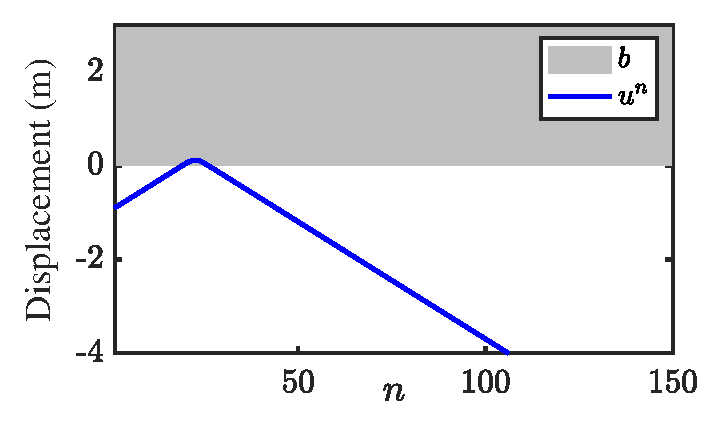
\includegraphics[width=\figWidth]{figures/interactions/massBarrierHigh.eps}}
    \caption{The mass -- rigid barrier collision over time with $\alpha_\text{c} = 1.3$ for different values of $K_\text{c}$. \label{fig:massBarrierCollision}}
\end{figure}


\subsection{Energy analysis}\label{sec:energyAnalysisMassBarrier}
To prove that the collision term does not add any additional energy into the system (retaining passivity) and that it does not add additional constraints on the stability of the system, the energy analysis techniques presented in Section \ref{sec:energyAnalysis} can be used. Notice that for brevity, the steps presented in Section \ref{sec:energyAnalysis} will not explicitly be followed.

Multiplying Eq. \eqref{eq:massBarrierSystem1} by $(\dtd \un)$ yields 
\begin{equation*}
    \dtp \h_\mtxt  = -\left(\mtp\psi^{n-1/2}\right)g^n (\dtd \un)
\end{equation*}
where the energy of the mass is defined as (see Eq. \eqref{eq:energyBalanceMassSpring})
\begin{equation}
    \h_\mtxt = \frac{M}{2}(\dtm\un)^2.
\end{equation}
Expanding $g^n$ yields 
\begin{align*}
    \dtp \h_\mtxt  &= -\left(\mtp\psi^{n-1/2}\right)\frac{\dtp \psi^{n-1/2}}{\dtd \eta^n}(\dtd \un)\\
    \xLeftrightarrow{\mystrut\ \text{Eq. \eqref{eq:derEtaEqDerU}}} \qquad & = -\left(\mtp\psi^{n-1/2}\right)\dtp \psi^{n-1/2},
\end{align*}
which, using identity \eqref{eq:prodIdentity3}, can be rewritten to 
\begin{equation}
    \dtp(\h_\mtxt + \h_\ctxt) = 0,
\end{equation}
with collision energy
\begin{equation}\label{eq:collisionEnergy}
    \h_\ctxt = \frac{(\psi^{n-1/2})^2}{2}.
\end{equation}
Recall that in order for a scheme to be passive, its energy must be non-negative, and the fact that $\psi$ is squared proves passivity for system \eqref{eq:massBarrierSystem}.

Figure \ref{fig:massBarrierEnergy} shows the energetic output of the mass -- rigid barrier collision corresponding to Figure \ref{fig:massBarrierLow}. The left panel shows that the kinetic energy of the mass is transferred into the energy of the collision, after which it is converted into kinetic energy of the mass again.

\begin{figure}[h]
    \centering
    \begin{tikzpicture}[->,node distance=3cm,
        thick,main node/.style={circle,draw}]
    
        \node[] (image) at (0,0) {
        \includegraphics[width=\textwidth]{figures/interactions/massBarrierEnergy.eps}
        };
    
        \node[] (he) at (0.2,0.5) {\small $\mathfrak{h}_\text{e}$};

        \node[] (h) at (-5.8, 1) {\small $\mathfrak{h}$};
        \node[] (t) at (-5.8, 0.5) {\small $\color{blue}\mathfrak{h}_\text{m}$};
        \node[] (v) at (-5.8, 0) {\small $\color{red}\mathfrak{h}_\ctxt$};

      \end{tikzpicture}
      \caption{The energy of the mass (blue), the collision (green) and the total energy (black) of the mass -- rigid barrier collision. The energy corresponds to the behaviour in Figure \ref{fig:massBarrierLow}. The right panel shows the normalised energy (according to Eq. \eqref{eq:normalisedEnergy}) shows that the deviation of the energy is within machine precision. \label{fig:massBarrierEnergy}}
\end{figure}

\section{Mass-spring -- string collision}\label{sec:massString}
The mass-spring -- string collision is slightly trickier than the mass -- rigid barrier collision, as there are two moving components rather than one. This system is chosen as an example as it has the interesting use-case of fretting a string to change the pitch, modelling the fretting finger as a mass.

Consider a lossless stiff string of length $L$, its transverse displacement described by $u = u(x,t)$ (in m) and defined for $t\geq 0$ and $x\in \D$ with domain $\D = [0, L]$. The mass with displacement $w = w(t)$ (in m) and $t\geq 0$ will model the fretting finger. The PDE for the stiff string and its parameter definitions can be found in Eq. \eqref{eq:stiffStringPDENoLosses} and for the mass-spring system in Eq. \eqref{eq:massSpringPDE}. Placing the string above the mass, the following system emerges:
\begin{subequations}\label{eq:massStringPDE}
\begin{align}   
    \rho A \ptt u & =T\pxx u - EI\pxxxx u + \delta(x-x_\text{m}) \psi g \label{eq:massStringPDE1}\\
    M \ddot w &=-Kw - \psi g\label{eq:massStringPDE2}\\
    \dot\psi &= g \dot\eta,\label{eq:massStringPDE3}\\
    \eta(t) &= w(t) - u(x_\text{m}, t),\label{eq:massStringPDE4}
\end{align}
\end{subequations}
where spatial Dirac delta function $\delta(x-x_\text{m})$ localises the mass (finger) along the string at location $x_\text{m} \in \D$ (see Eq. \eqref{eq:spatialDirac}). Furthermore, $\psi = \psi(\eta)$ and $g=\psi'$ are as defined in Eq. \eqref{eq:quadraticPotential}. 

Discretising system \eqref{eq:massStringPDE}, with the collision discretised according to the process explained in Section \ref{sec:massRigidBarrier}, yields
\begin{subequations}
    \begin{align}   
        \rho A \delta_{tt}u^n_l & =T\delta_{xx}u^n_l - EI\delta_{xxxx}u_l^n + J_l(x_\text{m}) \big(\mu_{t+}\psi^{n-1/2}\big)g^n, \label{eq:massString1}\\
        M \delta_{tt}w^n &=-Kw^n - \big(\mu_{t+}\psi^{n-1/2}\big)g^n,\label{eq:massString2}\\
        \delta_{t+}\psi^{n-1/2} &= g^n\delta_{t\cdot}\eta^n,\label{eq:massString3}\\
        \eta^n &= w^n - I_l(x_\text{m})\uln,\label{eq:massString4}
    \end{align}
\end{subequations}
where $l\in d$ with discrete domain $d=\{0, \hdots, N\}$ and number of grid points along the string $N+1$. Furthermore, spreading and interpolation operators $I_l(x_\text{m}) = I_{l, o}(x_\text{m})$ and $J_l(x_\text{m}) = J_{l, o}(x_\text{m})$ are as defined in Section \ref{sec:interpolationSpreading}. The order $o$ is left unspecified. Following the same process as in Section \ref{sec:solvingMassBarrier}, Eqs. \eqref{eq:massString1} and \eqref{eq:massString2} can be rewritten to 
\begin{subequations}\label{eq:massStringComb}
    \begin{align}
        \rho A \delta_{tt}u^n_l & =T\delta_{xx}u^n_l - EI\delta_{xxxx}u_l^n + J_l(x_\text{m}) \left(\frac{k}{2}g^n\delta_{t\cdot}\eta^n + \psi^{n-1/2}\right)g^n,\label{eq:massStringComb1}\\
        M \delta_{tt}w^n &=-Kw^n - \left(\frac{k}{2}g^n\delta_{t\cdot}\eta^n + \psi^{n-1/2}\right)g^n,\label{eq:massStringComb2}
    \end{align}
\end{subequations}
which can be used as a starting point for solving the system.

\subsection{Solving the system}
As the colliding objects are both moving, Eq. \eqref{eq:derEtaEqDerU} is not valid anymore and another strategy needs to be used.
To start, one must isolate the string at the collision location $x_\text{m}$ by taking an inner product of Eq. \eqref{eq:massStringComb1} with $J_l(x_\text{m})$ over discrete domain $d$. Using identity \eqref{eq:identityIJ} and dividing all terms by $\rho A$ yields
\begin{align*}
    \delta_{tt}I_l(x_\text{m})u^n_l =c^2I_l(x_\text{m})\delta_{xx}u^n_l &- \kappa^2I_l(x_\text{m})\delta_{xxxx}u_l^n \\
    &\quad + \frac{\lVert J_l(x_\text{m})\rVert^2_d}{\rho A} \left(\frac{k}{2}g^n\delta_{t\cdot}\eta^n + \psi^{n-1/2}\right)g^n.
\end{align*}
with $c = \sqrt{T/\rho A}$ and $\kappa = \sqrt{EI/\rho A}$. Expanding the temporal FD operators yields 
\begin{equation}\label{eq:stringMassunp1}
    I_l(x_\text{m})u_l^{n+1} = u^\star+ \underbrace{\frac{\lVert J_l(x_\text{m})\rVert^2_d k^2}{\rho A}}_{\mathfrak{J}_l} \left(\frac{(g^n)^2}{4}\left(\eta^{n+1}-\eta^{n-1}\right) + \psi^{n-1/2}g^n\right),
\end{equation}
where 
\begin{equation*}
    u^\star = I_l(x_\text{m})(2u_l^n -u_l^{n-1}) + c^2k^2I_l(x_\text{m})\delta_{xx}\uln- \kappa^2k^2I_l(x_\text{m})\delta_{xxxx}\uln
\end{equation*}
is the result of the update equation of the string at $x_\text{m}$ without the collision term. Then, Eq. \eqref{eq:massString4} evaluated at $n+1$, which is $\eta^{n+1} = w^{n+1} - I(x_\text{m})u_l^{n+1}$, can be substituted into Eq. \eqref{eq:stringMassunp1}, which results in
\begin{equation}\label{eq:expandedMassString1}
    \begin{aligned}
    \left(1 + \mathfrak{J}_l\frac{(g^n)^2}{4}\right)I_l(x_\text{m})u_l^{n+1} - \mathfrak{J}_l&\frac{(g^n)^2}{4} w^{n+1}= u^\star\\
    & + \mathfrak{J}_l \left(-\frac{(g^n)^2}{4}\eta^{n-1} + \psi^{n-1/2}g^n\right).
    \end{aligned}
\end{equation}
Performing this same process on the FD scheme of the mass in Eq. \eqref{eq:massStringComb2} yields
\begin{equation}\label{eq:expandedMassString2}
    \begin{aligned}
    -\frac{(g^n)^2 k^2}{4M} I_l(x_\text{m})u_l^{n+1} + &\left(1 + \frac{(g^n)^2 k^2}{4M}\right)w^{n+1} = w^\star\\
    & - \frac{k^2}{M} \left(-\frac{(g^n)^2}{4}\eta^{n-1} + \psi^{n-1/2}g^n\right),
    \end{aligned}
\end{equation}
where 
\begin{equation*}
    w^\star = 2w^n - w^{n-1} - \frac{Kk^2}{M}w^n
\end{equation*}
is (again) the result of the update equation of the mass without the collision term.
Equations \eqref{eq:expandedMassString1} and \eqref{eq:expandedMassString2} can be treated as a system of linear equations (see Section \ref{sec:linearEquations}) with unknowns $I_l(x_\text{m})u^{n+1}$ and $w^{n+1}$. Writing the aforementioned equations in matrix form yields
\begin{align}
    \begin{bmatrix}
            I_l(x_\text{m})u^{n+1}_l\\
            w^{n+1}
        \end{bmatrix}
        = 
        \mathbf{A}^{-1}\mathbf{v}
    \end{align}
    where
    \begin{equation}
    \begin{gathered}
    \mathbf{A} = 
        \begin{bmatrix}
            \left(1 + \mathfrak{J}_l\frac{(g^n)^2}{4}\right) & -\mathfrak{J}_l\frac{(g^n)^2}{4}\\
            -\frac{(g^n)^2 k^2}{4M} &\left(1 + \frac{(g^n)^2 k^2}{4M}\right)
        \end{bmatrix}
        \quad \text{and}\\
        \mathbf{v} = 
        \begin{bmatrix}
            u^\star + \mathfrak{J}_l \left(-\frac{(g^n)^2}{4}\eta^{n-1} + \psi^{n-1/2}g^n\right)\\
            w^\star- \frac{k^2}{M} \left(-\frac{(g^n)^2}{4}\eta^{n-1} + \psi^{n-1/2}g^n\right)
        \end{bmatrix}.
        \nonumber
    \end{gathered}
\end{equation}
From this, $\eta^{n+1}$ can be calculated, and can consequently be applied to the string and mass in system \eqref{eq:massStringComb}.

Figure \ref{fig:massStringCollision} shows an implementation of the mass spring collision. The mass is initialised with an upwards initial velocity, where $w^0 = -0.2, w^1 = -0.1$, and collides with the string almost instantly after the start of the simulation. As the first panel shows, the collision model allows for interpenetration of the objects. Immediately after, the collision force accelerates the string upwards and the mass downwards.

\begin{figure}[h]
    \centering
    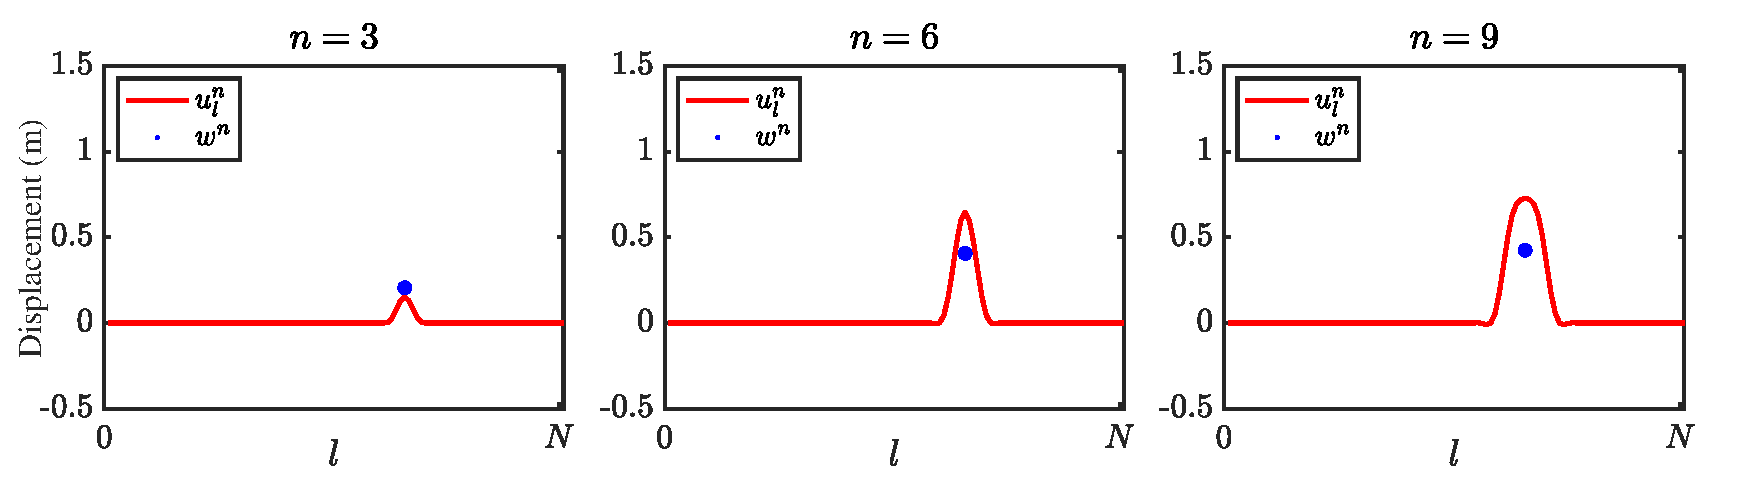
\includegraphics[width=\textwidth]{figures/interactions/stringMassCollision.eps}
    \caption{The collision of the mass (blue) and the string (red). The collision model allows for interpenetration of the objects as shown in the left panel. \label{fig:massStringCollision}}
\end{figure}

\subsection{Energy analysis}
This section follows Section \ref{sec:energyAnalysis} without explicitly following the steps for brevity. 

One can obtain the energy of the stiff string FD scheme in Eq. \eqref{eq:massString1} by taking the inner product of scheme by $(\dtd \uln)$ over discrete domain $d$ to obtain 
\begin{equation}\label{eq:rOCEnergyString}
    \dtp \h_\text{s} = \left\langle (\dtd \uln), J_l(x_\text{m})\left(\mtp \psi^{n-1/2}\right)g^n\right\rangle_d
\end{equation}
where the energy of the string is (see Eq. \eqref{eq:energyBalanceStiffString})
\begin{equation*}
    \begin{gathered}
        \h_\text{s} = \t_\text{s} + \v_\text{s}, \qwiq \t_\text{s} = \frac{\rho A}{2}\lVert\dtm \uln\rVert^2_d,\quad \text{and} \\
        \v_\text{s} = \frac{T}{2}\langle\dxp\uln, e_{t-}\dxp\uln\rangle_{\underline{d}} + \frac{EI}{2}\langle\dxx\uln, e_{t-}\dxx\uln\rangle_{\overline{\underline{d}}}\ .
    \end{gathered}
\end{equation*}
Energy analysis for the mass in Eq. \eqref{eq:massString2} can be done by multiplying the scheme by $(\dtd w^n)$ to get 
\begin{equation}\label{eq:rOCEnergyMass}
    \dtp \h_\text{m} = -(\dtd w^n)\left(\mtp \psi^{n-1/2}\right)g^n,
\end{equation}
where (see Eq. \eqref{eq:energyBalanceMassSpring})
\begin{equation*}
    \h_\text{m} = \t_\text{m} + \v_\text{m}, \qwiq \t_\text{m} = \frac{M}{2}(\dtm w^n)^2, \qaq \v_\text{m} = \frac{K}{2}w^n e_{t-}w^n.
\end{equation*}
The total energy in the system is the addition of Eqs. \eqref{eq:rOCEnergyString} and \eqref{eq:rOCEnergyMass}, which, using identity \eqref{eq:identityIJ} for the former, can be written as:
\begin{align*}
    \dtp(\h_\text{s} + \h_\text{m}) &= \Big(I_l(x_\text{m})(\dtd \uln) - (\dtd w^n)\Big)\left(\mtp \psi^{n-1/2}\right)g^n,\\
    &= \underbrace{\dtd\left(I_l(x_\text{m})\uln - w^n\right)}_{-\dtd \eta^n}\left(\mtp \psi^{n-1/2}\right)g^n.
\end{align*}
Then, expanding $g^n$ according to Eq. \eqref{eq:approxPsi} yields 
\begin{align*}
    \dtp(\h_\text{s} + \h_\text{m}) &= - \dtd\eta^n\left(\mtp \psi^{n-1/2}\right)\frac{\delta_{t+}\psi^{n-1/2}}{\delta_{t\cdot}\eta^n}\\
    &= -\left(\mtp \psi^{n-1/2}\right)\delta_{t+}\psi^{n-1/2}
\end{align*}
which, using identity \eqref{eq:prodIdentity3}, can be rewritten as
\begin{equation}
    \dtp(\h_\text{s} + \h_\text{m} + \h_\text{c}) = 0,
\end{equation}
with collision energy
\begin{equation*}
    \h_\text{c} = \frac{(\psi^{n-1/2})^2}{2}.
\end{equation*}
Again, the fact that $\psi$ is squared here, means that $\h_\text{c}$ is non-negative, and proves passivity of the system. 

Figure \ref{fig:massStringCollisionEnergy} shows the energy of the mass-spring collision corresponding to the behaviour shown in Figure \ref{fig:massStringCollision}. One can observe that energy of the mass is transferred to the string almost immediately after the start of the simulation. Furthermore, the figure shows that the mass and the string collide again at $n\approx 110$. The interpenetration of the two colliding objects can be observed from the small peaks in the value for $\h_\ctxt$ at these times. 

\begin{figure}[h]
    \centering
    \begin{tikzpicture}[->,node distance=3cm,
        thick,main node/.style={circle,draw}]
    
        \node[] (image) at (0,0) {
        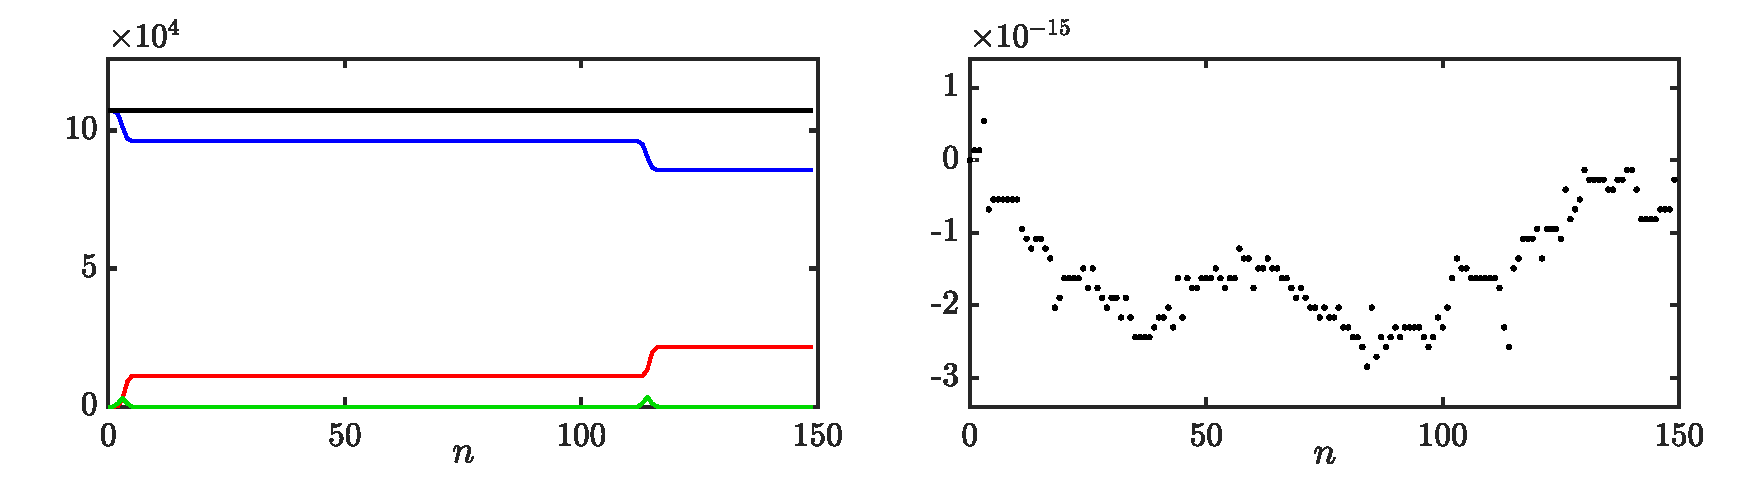
\includegraphics[width=\textwidth]{figures/interactions/stringMassCollisionEnergy.eps}
        };
    
        \node[] (he) at (0.2,0.5) {\small $\mathfrak{h}_\text{e}$};

        \node[] (h) at (-5.8, 1) {\small $\mathfrak{h}$};
        \node[] (t) at (-5.8, 0.5) {\small $\color{blue}\mathfrak{h}_\text{m}$};
        \node[] (v) at (-5.8, 0) {\small $\color{red}\mathfrak{h}_\stxt$};
        \node[] (c) at (-5.8, -0.5) {\small $\color[HTML]{00DB00}\mathfrak{h}_\ctxt$};

      \end{tikzpicture}
      \caption{The energy of the mass (blue), the string (red), the collision (green) and the total energy (black) of the mass-string collision. The energy corresponds to the system in Figure \ref{fig:massStringCollision}. The right panel shows the normalised energy (according to Eq. \eqref{eq:normalisedEnergy}) shows that the deviation of the energy is within machine precision. \label{fig:massStringCollisionEnergy}}
\end{figure}
\section{Two-sided collision: A connection}\label{sec:twoSidedCollision}

% As an alternative to the method connections shown in Chapter \ref{ch:connections} showed ways to connect various resonators using techniques presented in \cite{theBible}. An alternative method to establish these connections can be devised using the methods presented in this chapter.
% 

Using the methods presented in this chapter, one could devise a two-sided collision and alter the collision potential in Eq. \eqref{eq:potential} to \cite{Bilbao2019}
\begin{equation}\label{eq:twoSidedPotential}
    \phi(\eta) = \frac{K}{\alpha_\ctxt+1}|\eta|^{\alpha_\ctxt+1},
\end{equation}
and taking its derivative with respect to $\eta$ yields
\begin{equation}
    \phi'(\eta) = \sgn(\eta)K|\eta|^{\alpha_\ctxt}.
\end{equation}
One can observe that, as opposed to the (one-sided) potential presented in Eq. \eqref{eq:potential}, the collision force will be non-zero, for both a positive and negative $\eta$. This two-sided collision can be used as a connection -- as an alternative to connections presented in Chapter \ref{ch:connections} -- and has been used in papers \citeP[D] and \citeP[E] in combination with Eq. \eqref{eq:potential} to model the mechanics of the tromba marina. See Chapter \ref{ch:tromba} for more details.

% \part{Real-Time Implementation and Control}\label{part:realtime}
% \chapter*{Exciters}
Several resonators have been introduced in part \ref{part:resonators}, different mechanisms to excite them will be introduced here. First, different examples of 

and have a great effect on the eventual timbre of the sound. 
Chapter \ref{ch:physInspExcitations} presents various physically inspired excitations some of which made a brief appearance in Part \ref{part:resonators}. Chapter \ref{ch:bow} introduces a static and a dynamic friction model that can be used for bowing resonators. Additionally, this chapter presents the contribution made in \citeP[C]: the elasto-plastic friction model applied to FDTD stiff strings. Finally, Chapter \ref{ch:lipreed} presents the lip reed as a way to excite brass instruments. 

\input{realtime/realtimeImp}
\chapter{Control}

\section{Sensel Morph}
150 Hz

\section{Phantom OMNI}

\part{Contributions}\label{part:contributions}
\chapter*{Exciters}
Several resonators have been introduced in part \ref{part:resonators}, different mechanisms to excite them will be introduced here. First, different examples of 

and have a great effect on the eventual timbre of the sound. 
Chapter \ref{ch:physInspExcitations} presents various physically inspired excitations some of which made a brief appearance in Part \ref{part:resonators}. Chapter \ref{ch:bow} introduces a static and a dynamic friction model that can be used for bowing resonators. Additionally, this chapter presents the contribution made in \citeP[C]: the elasto-plastic friction model applied to FDTD stiff strings. Finally, Chapter \ref{ch:lipreed} presents the lip reed as a way to excite brass instruments. 

\newcommand{\dynamictitle}{Dynamic Grids}
\chapter*{\dynamictitle}\label{sec:dynamic}
\addcontentsline{toc}{chapter}{\dynamictitle}

\chapter*{Exciters}
Several resonators have been introduced in part \ref{part:resonators}, different mechanisms to excite them will be introduced here. First, different examples of 

and have a great effect on the eventual timbre of the sound. 
Chapter \ref{ch:physInspExcitations} presents various physically inspired excitations some of which made a brief appearance in Part \ref{part:resonators}. Chapter \ref{ch:bow} introduces a static and a dynamic friction model that can be used for bowing resonators. Additionally, this chapter presents the contribution made in \citeP[C]: the elasto-plastic friction model applied to FDTD stiff strings. Finally, Chapter \ref{ch:lipreed} presents the lip reed as a way to excite brass instruments. 

% \section{To do thingies}\label{sec:ch2label}
\begin{itemize}
  \item Think about how to define real-time.
\end{itemize}
% \chapter{Conclusions and Perspectives}\label{ch:conclusion}
\todo{title is the exact same as \cite{theBible}}
Both the good and bad thing about physical modelling musical instruments is that you are never done..

There is always more work to be done


\section{Realism}
We are not there yet.. 

Physical modelling is not here to replace the original instruments and the musicians playing them. Instead, it can be used as a tool to understand the physics of existing instruments and possibly go beyond. Simulated instruments are not restricted by physics anymore and could provide new ways of expression for the musician. 

\subsubsection{Parameter design}
Many parameters that can always be improved

Possible perspectives could be machine learning based on audio files (literature...)

\section{Dynamic grid}
In this work, the dynamic grid in Chapter \ref{ch:dynamicGrid} the test case of the 1D wave equation has been explored. 

% {\small\bibliographystyle{IEEEtranS}\bibliography{bib/mybib}}

\chapter{Real-Time Implementation and Control}\label{ch:realtime}

\begin{flushright}{\it
    ``The real problem is that programmers have spent far too much time worrying \\
    about efficiency in the wrong places and at the wrong times; premature\\
    optimization is the root of all evil (or at least most of it) in programming.''\\
    - Donald E. Knuth}
\end{flushright}
%
\vspace{2em}
\todo{check if all references to this chapter are actually touched upon in here}
\noindent A large part of this PhD project has been to implement novel combinations of existing FD schemes in real time (see Section \ref{sec:objectivesContributions}). As opposed to many FDTD-based musical instruments found in the literature, those presented in this work, allow for real-time control such the virtual instrument can be played. 

Many simulations are focused on accuracy and

Real-time implementations of FD schemes 

physical models
Give overall structure of code

Important to find the balance between accuracy and sound. 

Implementation of the physical models
using FDTD methods

As mentioned in Chapter \ref{ch:physMod}, FDTD methods are used for high-quality and accurate simulations, rather than for real-time applications. This is due to their lack of simplifications.

Usually, \texttt{MATLAB} is used for simulating 

Here, an interactive application is considered real-time when
\begin{center}\it
    Control of the application generates or manipulates audio with no noticeable latency.
\end{center}

For human-computer interaction, the task at hand greatly determines how much latency is acceptable. Wessel and Wright \cite{Wessel2002} place the upper limit of latency when interacting with computers for musical purposes at $10$ ms. Moreover, they place the a limit on the \textit{jitter}, or of variation of the latency, at $1$ ms. It is thus important to keep the CPU usage at a fixed level as much as possible, and different ways of controlling and interacting with the application should not influence the number of computations much.

Also the application needs to be controlled continuously

As a large contribution of this PhD project was the real-time implementation of the physical models presented in 

Finite representation: $1.80\cdot 10^{308}$


Apart from being able to be used by musicians, real-time implementations can truly help to (informally) evaluate the models by interacting with it in a natural way (rather than static parameters).


\todo{Figure with programming languages sorted by speed}




Although \texttt{MATLAB} is a great tool for prototyping, it is a \textit{high-level} programming language, i.e., has a high level of abstraction. Generally, higher-level programming languages are easier to program, but more control -- and speed -- is gained by using a lower-level programming language such as C++.

It must be said that \texttt{MATLAB} is highly optimised for large matrix computations.

A great framework for real-time audio programming is provided by JUCE.\footnote{\url{https://juce.com/}} This framework provides functionality that handles the backend of  an application and specifically allows for audio and graphics to run simultaneously on separate threads. All real-time instrument simulations made over the course of this PhD project have been implemented using the JUCE framework. 


some details on this will be given. 
This chapter provides information on the real-time implementations made during this PhD project

This chapter can be considered a general contribution that can be applied to all papers in Part \ref{part:papers} (except paper \citeP[G]). The most important aspects of the implementation will be highlighted.

Firstly, details on the structure of a class implementing a FD scheme will be provided, using the damped stiff string as an example. Secondly, an overall code structure is given that can be applied to many applications created during this PhD project.   

Then... 

Finally, this chapter will present the Sensel Morph and the PHANTOM Omni, two hardware devices which have been used to control the physical models presented in papers \citeP[A], \citeP[B], \citeP[C], \citeP[D] and \citeP[E].

\section{Real-time FD schemes}\label{sec:realTimeFDScheme}
Until now, this thesis presented matrix form of schemes (see e.g. Eqs. \eqref{eq:matrixFormStiffString} and \eqref{eq:matrixFormThinPlate}) for a compact implementation in \texttt{MATLAB}. Although libraries for handling matrices in C++ exist, the highest algorithm speed is obtained by using the update equations directly.

In any of the real-time applications created during this project, the update equation implementing an FD scheme is always most computationally expensive part. This algorithm needs to run 44100x per second, whereas the rest of the implementation can run at a much lower rate. This section provides details and considerations on the real-time implementation of FD schemes in C++ during this project. The damped stiff string presented in Chapter \ref{ch:stiffString} will be used an example. The full implementation can be found online and parts will be presented here to aid the explanation.\footnote{\url{https://github.com/SilvinWillemsen/SimpleStringApp/}} The FD scheme is implemented in a separate class called \texttt{SimpleString}, and will be used in the following explanation.

% Before going into the implementation of the update equation, this section provides the setup necessary for the implementation.

\subsection{System states and pointer switches}\label{sec:pointerSwitch}
In any FD scheme implementation, at the end of every iteration, the system states must be updated, i.e., the following operations must be performed:
\begin{equation*}
    \u^{n-1} := \u^{n} \qaq \u^{n} := \u^{n+1}.
\end{equation*}
In \texttt{MATLAB}, one would simply perform these operations according to

\setlstMAT
\begin{lstlisting}[belowskip=-0.5\baselineskip]
for n = 1:lengthSound
    ...
    uPrev = u;
    u = uNext;
end
\end{lstlisting}
In C++, however, one has the ability to perform a \textit{pointer switch} to update the system states. For a 1D FD scheme with $N+1$ grid points, the number of copy-operations it takes to update the system states manually would be $2(N+1)$, as shown in Figure \ref{fig:vectorCopy}. A pointer switch, as shown in Figure \ref{fig:pointerSwitch}, only needs 4 copy-operations per iteration and can be carried out in C++ as follows:

\setlstCpp
\begin{lstlisting}[belowskip=-0.5\baselineskip]
double SimpleString::updateStates()
{
    double* uTmp = u[2];
    u[2] = u[1];
    u[1] = u[0];
    u[0] = uTmp;
}
\end{lstlisting}
Here, \texttt{u} is a vector containing 3 pointers, each of which points a state vector at a certain time step: 
\begin{equation}
    \texttt{u[0]} \rightarrow \u^{n+1}, \quad \texttt{u[1]} \rightarrow \u^{n}, \qaq \texttt{u[2]} \rightarrow \u^{n-1}.
\end{equation}
A temporary pointer is assigned to where the $\u^{n-1}$ pointer is currently pointing at, to be able to assign that location in memory to the $\u^{n+1}$ pointer in the end. The values of that vector will be overwritten by the update equation in the next iteration (see Section \ref{sec:updateEquationCpp} and Figure \ref{fig:pointerSwitchFull}).

\begin{figure}[t]
    \centering
    \subfloat[Copying values: $2(N+1)$ operations per iteration. \label{fig:vectorCopy}]{\includegraphics[width=0.8\textwidth]{figures/realtime/vectorCopy.pdf}}\\
    \subfloat[Pointer switch: 4 operations per iteration. \label{fig:pointerSwitch}]{\includegraphics[width=0.8\textwidth]{figures/realtime/pointerSwitch.pdf}}
    \caption{Updating the state vectors by (a) copying all values individually, or (b) performing a pointer switch. Non-zero values are highlighted in green for clarity. The values of the red vector will be overwritten by the update of the scheme in the next iteration so these values will no longer be used.\label{fig:pointerSwitchFull}}
\end{figure}

The state vectors themselves are stored in a matrix (which is a `vector of vectors' in C++). This matrix will have 3 columns related to the 3 time steps required in the FD scheme, and $N+1$ rows, which is the number of grid points.\footnote{These are not actual rows and columns as in a matrix, but are used here for ease of explanation.} The matrix is initialised as follows

\setlstCpp
\begin{lstlisting}[belowskip=-0.5\baselineskip]
//// In the constructor of SimpleString////

// initialise vectors
uStates = std::vector<std::vector<double>> (3, 
                                    std::vector<double>(N+1, 0));
\end{lstlisting}
%
Next, the aforementioned pointers are initialised such that they contain the to the memory addresses of the first indices of the three state vectors in the matrix.

\begin{lstlisting}[belowskip=-0.5\baselineskip]
//// In the constructor of SimpleString ////

// Initialise pointer vector
u.resize (3, nullptr);

// Make set memory addresses to first index of the state vectors.
for (int i = 0; i < 3; ++i)
    u[i] = &uStates[i][0];
\end{lstlisting}
One will then be able to work with the pointers directly in the eventual update equation (see Section \ref{sec:updateEquationCpp}).

\subsection{Precalculation}
To prevent extra computations in the FD scheme, one wants to calculate as many of the coefficients possible beforehand, as these (generally) do not vary over time. Recalling the update equation for a stiff string in Eq. \eqref{eq:stiffStringUpdate}, one can write this as
\begin{equation}
    \begin{aligned}
        A_\text{div} u_l^{n+1} &= B_1 \uln + B_2 (u_{l+1}^n + u_{l-1}^n) + B_3(u_{l+2}^n + u_{l-2}^n) \\
        &\quad+ C_1u_l^{n-1}+ C_2(u_{l+1}^{n-1} + u_{l-1}^{n-1}),
    \end{aligned}
    \end{equation}
where
\begin{gather*}
    A_\text{div} = 1+\sz k, \quad B_0 = 2 - 2\lambda^2 - 6\mu^2 - \frac{4\so k}{h^2}, \quad B_1 = \lambda^2 + 4\mu^2 + \frac{2\so k}{h^2},\\
    B_2 = - \mu^2, \quad C_0 = -1+\sz k + \frac{4\so k}{h^2},\qaq C_1 = - \frac{2\so k}{h^2}.
\end{gather*}
All these coefficients can be calculated in the constructor of the stiff string class. One can also already divide the $B$ and $C$ coefficients by $A_\text{div}$ as done in the code below.
\setlstCpp
\begin{lstlisting}[]
//// In the constructor of SimpleString ////

// Coefficients used for damping
S0 = sigma0 * k;
S1 = (2.0 * sigma1 * k) / (h * h);

// Scheme coefficients
B0 = 2.0 - 2.0 * lambdaSq - 6.0 * muSq - 2.0 * S1; // u_l^n
B1 = lambdaSq + 4.0 * muSq + S1;                   // u_{l+-1}^n
B2 = -muSq;                                        // u_{l+-2}^n
C0 = -1.0 + S1 + 2.0 * S2;                         // u_l^{n-1}
C1 = -S1;                                          // u_{l+-1}^{n-1}

Adiv = 1.0 / (1.0 + S0);                           // u_l^{n+1}

// Divide by u_l^{n+1} term
B0 *= Adiv;
B1 *= Adiv;
B2 *= Adiv;
C0 *= Adiv;
C1 *= Adiv;
\end{lstlisting}

\subsection{Update equation}\label{sec:updateEquationCpp}
With all the above set up, the update equation can be implemented as follows:

\begin{lstlisting}[belowskip=-0.5\baselineskip]
void SimpleString::calculateScheme()
{
    for (int l = 2; l < N-1; ++l) // clamped boundaries
            u[0][l] = B1 * u[1][l] + B2 * (u[1][l + 1] + u[1][l - 1]) 
                + B3 * (u[1][l + 2] + u[1][l - 2])         
                + C1 * u[2][l] + C2 * (u[2][l + 1] + u[2][l - 1]);
}
\end{lstlisting}
This function and the pointer switch in Section \ref{sec:pointerSwitch} (in that order) will then have to be called once per sample.


\section{Code structure}\label{sec:codeStructure}
This section presents the general code structure used for the real-time applications created in this project. As an example, consider a simple instrument consisting of one string and one plate, and a connection between them as presented in Section \ref{sec:stringPlateConnection}. The string is excited using the Sensel Morph (see Section \ref{sec:sensel}). This is a simplified case of the contribution made in papers \citeP[A] and \citeP[B]. 

The structure of the code is visualised in Figure \ref{fig:codeStructure}. The white boxes denote various classes or components of the application which will be described in detail shortly. The black arrows indicate instructions, and hollow arrows indicate data flows. All arrows are accompanied by a box denoting the instruction / dataflow and the colour of the box denotes at what rate this happens.

\begin{figure}[h]
    \centering
    \includegraphics[width=0.8\textwidth]{figures/realtime/flowchart.pdf}
    \caption{The structure of a real-time implementation of a physical model. Boxes with `u \& o' refer to `update and output' and `Inter.' is short for `Interaction'. A detailed description of the figure is given in Section \ref{sec:codeStructure}. (Adapted from paper \citeP[A])\label{fig:codeStructure}}
\end{figure}

\subsubsection{Threads}
The application contains three different threads, all handled by the JUCE backend. The highest priority thread is the audio thread and is denoted by orange blocks. It runs at 44100 Hz and handles the calculations of the FD schemes. Denoted by blue, is the control thread and runs at 150 Hz. The input from the Sensel will be applied to the application at this rate. This rate corresponds to a maximum \textApprox 7 ms latency in control, which is below the upper limit for latency in musical applications proposed in \cite{Wessel2002}. Finally, the thread updating the graphical user interface (GUI) is set to run at 15 Hz, which is a value that was heuristically found to be a good balance between a smooth visuals and a fast application. %For powerful computers, or for low-complexity physical models, the speed could be increased. 
Papers \citeP[A], \citeP[C], and \citeP[H], contain a comparison between the speed of the application with and without the graphics. In all cases, results show that the graphics take up a large part of the computational power available.

\subsubsection{String and Plate}
The String and Plate classes implement the FD schemes of the stiff string and thin plate resonators respectively.\footnote{Note that the class can not actually be called `String' as this is already an existing variable type.} See Section \ref{sec:realTimeFDScheme} for an example of an implementation of the stiff string; a similar code structure can be used for the Plate class. As this section follows Section \ref{sec:stringPlateConnection}, the grid functions describing the string and the plate are defined as $\uqn$ and $\wlmn$, respectively. 

For the resonators to work in isolation, both classes require a function that calculates the scheme and one that updates their system states (see Section \ref{sec:realTimeFDScheme}). The interactions between the classes is handled by the Instrument class (see below). Therefore, both classes require additional functions that return $u^\star$ and $w^\star$ (see Figure \ref{fig:codeStructure}), as well as a function that adds the interaction force $f^n$ to the schemes. A final function on the audio  

Finally, the classes contain a `paint' function called by the GUI thread that visualises their state to the screen. 

\subsubsection{Instrument}
The Instrument class contains instances of the individual resonators and calls the functions that calculates the schemes and updates the states.

is called from the Main Application and contains instances of the individual resonators. Rather than performing the calculations of the FD schemes of these resonators, the Instrument class handles all interactions between the individual resonators. In the figure, this is denoted by the `Inter.' block and proceeds as follows:
\begin{enumerate}
    \item The instrument class retrieves the states of the schemes without the connection force. These are denoted by $u^\star$ and $w^\star$ and are calculated using in Eqs. \eqref{eq:stringPlateUStar} and \eqref{eq:stringPlateWStar}). These calculations are done in the String and Plate classes respectively (see below).
    \item The connection force $f^n$ is calculated using Eq. \eqref{eq:stringPlateForce}.
    \item The force is added to the scheme. 
\end{enumerate}

by the  the interaction between the string and the plate -- denoted by the `Inter.' block -- will be handled by the instrument class. It obtains the data needed to solve 

describes the interaction between the string and the plate and will be solved in the instrument class. 



The individual resonators could 


\subsubsection{Main Application}
The Main Application (also called MainComponent in JUCE) is the top-level class of the application that handles the audio input and output\footnote{This section assumes that the JUCE Audio Application template has been chosen -- not the Audio Plugin template.}

The main application contains an instance of the instrument class and calls a function 

Furthermore, it retrieves the output from the instrument which in turn retrieves it from the individual resonators.


Here, the interaction with the system is handled audio is handled.

Contains an instance of the instrument class


\subsection{Control}
Finally, the Sensel controls the application

Using the JUCE built-in HighResTimer class. For the real-time control of any application using FD schemes, whether it uses the mouse or an external controller, the important thing is to receive an excitation or a change in a control parameter outside of the scheme calculation.

It might happen that 

(preferably outside of the buffer



\section{Optimisation strategies}
This section provides several optimisation strategies that can be used for faster implementations. Although not all of these have not been used

\subsection{Code}
Much optimisation can already be done in the code itself 


\subsubsection{Grouping terms and precalculating coefficients}
Generally in implementations of FD schemes the most computationally expensive part of the algorithm is the calculation of the scheme itself. This is due to the rate at which it needs to be updated which usually is 44100 Hz. Graphics can be updated at rates orders of magnitude lower than the audio (\textApprox 60 Hz) and still be considered smooth enough.

Recall the update equation for the 1D wave update equation in Eq. \eqref{eq:1DwaveUpdate}
\begin{equation*}
    u_l^{n+1} = (2 - 2 \lambda^2) \uln - u_l^{n-1} + \lambda^2\left(u_{l+1}^n + u_{l-1}^n\right).
\end{equation*}
Grouping the terms like this allows for the coefficients multiplied onto the grid function at different temporal and spatial indices to be precomputed. This can significantly decrease the number of operations per sample.

The undamped stiff string FD scheme%in \eqref{eq:stiffStringFDS}
\begin{equation}
    \dtt \uln = c^2 \dxx \uln - \kappa^2 \dxxxx \uln,
\end{equation}
can be expanded to an update equation as
\begin{equation}
    \begin{aligned}
        u_l^{n+1} = &\ 2\uln - u_l^{n-1} + \lambda^2 \left(u_{l+1}^n - 2\uln + u_{l-1}^n\right)\\
        & - \mu^2 \left(u_{l+2}^n - 4u_{l+1}^n + 6\uln + -4u_{l-1}^n + u_{l-2}^n\right)
    \end{aligned}
\end{equation}
where $\lambda = ck/h$ and $\mu = \kappa k / h^2$.

For implementation purposes there is a better way to write this scheme that reduces the number of computations. This is done by collecting the terms based on the grid function and pre-calculating the coefficients multiplied onto these. As the schemes are spatially symmetric, ``neighbouring points'' relative to $\uln$ can also be grouped to get
\def\semilarge{\fontsize{11}{11.6}\selectfont}
\begin{equation}
    u_l^{n+1} = \underbrace{(2 - 2\lambda^2 - 6\mu^2)}_{\texttt{\semilarge B1}}\uln  + \underbrace{\left(\lambda^2 + 4\mu^2\right)}_{\texttt{\semilarge B2}}\left(u_{l+1}^n+u_{l-1}^n\right)\underbrace{-\mu^2}_{\texttt{\semilarge B3}} \left(u_{l+2}^n+u_{l-2}^n\right) \underbrace{-}_{\texttt{\semilarge C1}} u_l^{n-1}.
\end{equation}
These coefficients can then be pre-calculated and do not have to be 



\cite{Webb2015}
AVX GPU etc..\cite{Bilbao2019CMJb}



\section{Matrices}\label{sec:realTimeMatrices}

Library called \textit{Eigen} \cite{Eigen}

\subsection{Matrix inversions in real-time}\label{sec:RTmatrixInversion}
For small ($2\times 2$ and $3\times 3$) matrices it is doable to do the inversion `by hand'. This requires finding the \textit{determinant} of a matrix

\begin{equation*}
    \u = \A^{-1}\w, 
\end{equation*}
where
\begin{equation}
    \A^{-1} = \frac{1}{a_{00}\cdot a_{11} - a_{01}\cdot a_{10}}
    \begin{bmatrix}
        a_{11} & -a_{01}\\
        -a_{10} & a_{00} 
    \end{bmatrix}
\end{equation}

\setlstCpp
\begin{lstlisting}
det = a00 * a11 - a01 * a10;
u0 = (w0 * a11 - w1 * a01) / det;
u1 = (-w0 * a10 + w1 * a00) / det;
\end{lstlisting}


The computational complexity of th inversion of an $n\times n$ matrix is (at worst) $\OO(n^3)$. For real-time applications, the size of matrices one wants to invert thus need to be kept to a minimum...

The difference between inverting a $2\times 2$ matrix and a $3\times 3$ 

\section{Control}
Throughout this project, two hardware devices to expressively control the simulated instruments have been investigated. These are the Sensel Morph and the PHANTOM Omni, both of which will be briefly described here. The mapping of these controllers to the various instrument simulations can be found in the respective papers in Part \ref{part:papers}. 

\subsection{Sensel Morph}\label{sec:sensel}
The \textit{Sensel Morph,} or Sensel for short, is a high-accuracy pressure sensitive touch controller containing \textApprox 20,000 pressure-sensitive sensors that allow for high-fidelity application control (see Figure \ref{fig:sensel})\footnote{https://sensel.com/}

The controller has been used to control the physical models in  paper

Papers \citeP[A] and \citeP[B] were the first scientific papers to use the Sensel to control a musical instrument simulation (or even the first scientific papers to include the Sensel at all). Afterwards, the controller was used for controlling other applications. See e.g. \cite{Paisa2019,Pardue2020,vanWalstijn2021}

For this project, the Sensel has mainly been used for controlling the bow to excite stiff strings  in papers \citeP[A] and \citeP[B], \citeP[C] and \citeP[D]. Additionally

\begin{figure}[h]
    \centering
    \includegraphics[width=0.8\textwidth]{figures/contributions/realtime/senselHands.jpg}
    \caption{The Sensel Morph. \label{fig:sensel}}
\end{figure}

% \begin{figure}[h]
%     \centering
%     \includegraphics[width=\textwidth]{figures/realtime/dimensions.jpg}
%     \caption{Dimensions of the Sensel morph. (Taken from Sensel website with permission.) \label{fig:senselDims}}
% \end{figure}


\subsection{PHANTOM Omni}\label{sec:phantomOmni}
The PHANTOM Omni, or Omni for short, is a six-degrees-of-freedom device that provides force and vibrotactile feedback (see Figure \ref{fig:omni})

Other work using the Omni in a musical context, specifically for plucking a virtual guitar string, was done by Passalenti et al. in \cite{passalenti2019a, passalenti2019b} and Fontana et al. in \cite{Fontana2020}

\begin{figure}[h]\includegraphics[width=0.8\textwidth]{figures/contributions/realtime/omniSchematic.png}
    \centering
      \caption{The PHANTOM Omni haptic device. The device has six axes of rotation (6-DoF), three of which provide force feedback (A1-3), and three that only track position (B1-3). \label{fig:omni}}
\end{figure}

\section{Discussion and Conclusion}
No proper comparisons have been done between MATLAB and C++

examples can be found in \cite{Webb2015} and \cite{Bilbao2019CMJb}





\subsection{Translating MATLAB to C++}
Indexing in
Matlab is 1-based, meaning that the index of a vector starts at 1. If \texttt{u} is a vector with 10 elements, the first element is retrieved as \texttt{u(1)} and the last as \texttt{u(10)}. C++, on the other hand, is 0-based and retrieving the first and last element of a size-10 vector happens through \texttt{u[0]} and \texttt{u[9]}respectively. 

\section{Considerations in real-time FD schemes}

Some of the things I learned (the hard way)...
\begin{itemize}
    \item Create a limiter
    \item Structure your application into classes 
    \item Use pointer switches
    \item Comment your code (hehe)
    \item Working with JUCE: select your audio output before building the application...
\end{itemize}

\subsubsection{Create a limiter}
Programming errors happen. To save your speakers, headphones or -- most importantly -- your ears, create a limiter. 

\setlstCpp
\begin{lstlisting}
double limit (double val)
{
    if (val < -1)
    {
        val = -1;
        return val;
    }
    else if (val > 1)
    {
        val = 1;
        return val;
    }
    return val;
}
\end{lstlisting}

\setlstMAT
\begin{lstlisting}
for  i = 0:lengthSound
    uNext = ...
end
\end{lstlisting}

\subsubsection{Denormalised numbers}
The damping present in FD schemes causes the state of the system to exponentially decay. What this means for the values of the state vectors in implementation, is that they keep getting closer to $0$ but never reach it. 

After a long period of time, which depends on the value of the damping coefficients, state values can get in the range of \textApprox$10^{-307}$! Numbers in this range are referred to as \textit{denormalised numbers} and operations with these are ``extremely slow'' \cite{CPPdenormalised}.

Although it rarely happens that numbers end up in this range, especially when the application is continuously interacted with, it is good to account for the possibility. For example, due to the very high damping of the body in the Tromba Marina application in Chapter \ref{ch:tromba}, denormalised numbers appear after \textApprox 10 s of not interacting with the instrument, and the CPU usage shoots up. There are specific processor flags that can be activated to truncate denormalised numbers to 0. To retain generality (cross-platform, various processors), one could implement a simple check per buffer to see whether values are smaller than e.g. $10^{-250}$ and truncate all values of that system to $0$. 


\section{Considerations for translating MATLAB to C++}
Although the \texttt{MATLAB} language, referred to throughout this thesis, is an excellent prototyping tool

This section will provide some considerations when moving from MATLAB to C++ 

It is usually a good idea to prototype a physical modelling application in \texttt{MATLAB} for various reasons, but  reasons: 1) Easier to debug, 2) Plotting functionality, 3) No need for memory handling, 4) no headphone blowup due to instability through programming errors




\chapter{Large Scale Modular Physical Models}\label{ch:largeScale}
This chapter provides an extended summary for the work presented in the papers ``Real-Time Control of Large-Scale Modular Physical Models using the Sensel Morph'' \citeP[A] and ``Physical Models and Real-Time Control with the Sensel Morph'' \citeP[B].  Paper \citeP[A] presents the work done on various physical models connected by nonlinear springs using three instruments as case studies: the esraj (bowed sitar), the hammered dulcimer and the hurdy gurdy. The implementations and a video showcasing the hurdy gurdy can be found online.\footnote{\url{https://github.com/SMC-AAU-CPH/ConnectedElements/releases/tag/v5.0}}\textsuperscript{,}\footnote{\url{https://youtu.be/BkxLji2ap1w}} Paper \citeP[A] follows \cite{theBible} and \cite{Bilbao2009Modular} and uses `scaling' (see Section \ref{sec:1DwaveContTime}). To relate the paper to the theory presented in this thesis, this chapter presents the models in a non-scaled, dimensional form. The eventual implementation of the models is equivalent. Then, a summary of the remaining parts of the paper is provided, including descriptions of the instruments.
% Furthermore, this chapter will build on the contents of paper \citeP[A] by providing more details on the implementation.\todo{will it though?}

\section{Physical models}\label{sec:modelsLargeScale}
All instruments use multiple instances of the stiff string presented in Chapter \ref{ch:stiffString} and one instance of the thin plate presented in Section \ref{sec:thinPlate}. The latter was used as a simplified instrument body for the resulting simulations (see Section \ref{sec:largeScaleInstruments}). Theory on connections can be found in Chapter \ref{ch:connections}, and information on the string-plate connection, specifically, is presented in Section \ref{sec:stringPlateConnection}.

Consider a set of strings, where the transverse displacement of string $s$ is described by $u_s = u_s(\chi_s, t)$ (in m) defined for $t\geq 0$ and $\chi_s \in \D_s$ for domain $\D_s = [0, L_s]$ and length $L_s$ (in m). Notice that every string is defined for a separate coordinate system $\chi_s$. In the following, spatial derivatives $\partial_{\chi_s}$ are the same as those described in Section \ref{sec:FDoperators}, but with respect to coordinate $\chi_s$. The PDE of string $s$ with an external connection force is defined as %(after division by $\rho_sA_s$)
\begin{equation}
    \begin{aligned}
    \ptt u_s = c_s^2 \partial_{\chi_s\chi_s} u_s &- \kappa_s^2 \partial_{\chi_s\chi_s\chi_s\chi_s} u_s - 2 \szX[s]\pt u_s\\
    &\quad + 2 \soX[s] \partial_{\chi_s\chi_s} u_s - \delta(\chi_s - \chi_{s, \ctxt})\frac{f_s}{\rho_sA_s},
    \end{aligned}
\end{equation}
where spatial Dirac delta function $\delta(\chi_s - \chi_{s,\ctxt})$ (in m$^{-1}$) localises the connection force between the string $s$ and the plate to connection location $\chi_{s, \ctxt}$. Other parameters are as defined in Eq. \eqref{eq:stiffStringPDE} but have a subscript $s$ to denote that they can be different for each strings. 

As all connections in the implementation are between an individual string and the plate, the PDE of the thin plate in Eq. \eqref{eq:platePDE} can be extended to 
\begin{equation}
    \begin{aligned}
    \!\!\!\!\ptt w = -\kappa_\ptxt^2\Delta\Delta w &\!-\! 2\szX[\ptxt]\pt w\! +\! 2\soX[\ptxt] \pt\pxx w+ \!\sum_s\delta(x \!-\! x_{\ctxt,s}, y \!-\! y_{\ctxt,s})\frac{f_s}{\rho_\ptxt H},\!\!\!\!\!\!
    \end{aligned}
\end{equation}
where 2D spatial Dirac delta function $\delta(x_s - x_{s,\ctxt}, y_s - y_{s,\ctxt})$ (in m$^{-2}$) localises the connection force of between the plate and string $s$ to coordinate $(x_s, y_s)$ on the plate. Other parameters are as defined in Eq. \eqref{eq:platePDE}. 

Finally, the connection force between the plate and string $s$ is defined as a nonlinear damped spring (see Eq. \ref{eq:nonlinearForce})
\begin{equation}
    f_s = K_1\eta_s + K_3\eta_s^3 + R \dot \eta_s,
\end{equation}
where
\begin{equation}
    \eta_s = u_s(\chi_{\ctxt,s}, t) - w(x_{\ctxt,s}, y_{\ctxt,s}, t)
\end{equation}
is the relative displacement between string $s$ and the plate at their respective connection locations. Notice that the plate is placed below the strings such that the sign of the force term is negative for the strings and positive for the plate.

\section{Implementation}
This section provides considerations for implementing the above models. Details on discretisation of the models and how to solve for $f_s$ are presented in Section \ref{sec:stringPlateConnection} and are not given here. 

The spatial Dirac delta functions are discretised using 0\thOrder spreading operators for simplicity (see Section \ref{sec:interpolationSpreading} (1D) and Section \ref{sec:interpolationSpreading2D} (2D)). Furthermore, the connection locations on the plate are implemented to be non-overlapping. Overlaps would require to solve a system of linear equations to obtain the connection forces (see e.g. \cite{Bilbao2009Modular}). Looking towards real-time implementation, an explicit solution for each connection is desired.

\section{Summary}
This section provides a summary of the instrument simulations presented in paper \citeP[A]. All instruments were implemented in real-time in C++ using the JUCE framework (see Chapter \ref{ch:realtime}). Finally, a summary of the results and the conclusion will be given.

\subsection{Instruments}\label{sec:largeScaleInstruments}
Using the setup presented in Section \ref{sec:modelsLargeScale}, various configurations inspired by real instruments have been made. The choices of simulated instruments were aimed at those containing many (sympathetic) strings.\footnote{Sympathetic strings -- apart from being friendly -- are strings that add resonances to the instrument without being excited directly.} Another condition was that no FDTD-based physical models existed in the literature at the time of writing the papers.

Three implementations inspired by real-life instruments were created and their setups are presented here. The implementations were controlled by a pair of Sensel Morph controllers (see Section \ref{sec:sensel}). The mapping between the controllers and the instruments is explained in papers \citeP[A] and \citeP[B].

\subsubsection{Esraj: bowed sitar}
The first instrument simulation was inspired by the \textit{esraj}: the bowed sitar. This instrument uses many strings, some of which are bowed and others are sympathetic strings that resonate when the instrument is played. As one can also interact with the latter, several strings in the implementation could be plucked as well. 

In total, 20 strings were implemented, all connected to a thin plate: 2 strings could be bowed, 5 strings could be plucked, and 13 strings are sympathetic. The bow was implemented using the static friction model presented in Section \ref{sec:staticFricMod} and the pluck was modelled as a time-varying raised cosine found in Section \ref{sec:timeVaryingRaisedCos}.

\subsubsection{Hammered dulcimer}
The hammered dulcimer, or santur, can be seen as an `open piano' where the player hammers several strings at once. In the implementation, 20 pairs of strings are implemented, and one in each pair is connected to the plate. This causes a slight detuning between the strings, resulting in a characteristic `chorus' effect exhibited by the instrument. To excite the strings, the time-varying strike presented in Section \ref{sec:timeVaryingRaisedCos} is used.

\subsection{Hurdy gurdy}
The hurdy gurdy is a bowed string instrument, that also uses sympathetic strings. Rather than a bow, the instrument uses a rosined wheel attached to a crank that bows the strings as it is turned. As for the esraj, the static friction model presented in Section \ref{eq:staticFriction} was used to implement the wheel. 

The instrument simulation consists of 5 bowed strings and 13 sympathetic strings, all connected to a plate. 

\subsection{Results and conclusion}
All instrument simulations were able to run in real time on a MacBook Pro with a 2.2 GHz Intel i7 processor.
Interaction with the implementations shows that when exciting one string, the connections with the plate cause other (sympathetic) strings to vibrate as well. Specifically, strings tuned to one of the harmonic partials of the excited string were found to resonate to a high degree. This phenomenon is consistent to real-world processes.

Finally, informal evaluations of the instruments were carried out on experts in the sound and music computing field, and showed that the mapping between the Sensels and the instruments, specifically the bowing interaction, was considered natural and intuitive.
\chapter{Tromba Marina}\label{ch:tromba}
This chapter presents the work done in the papers ``Real-time Implementation of a Physical Model of the Tromba Marina'' \citeP[D] and ``Resurrecting the Tromba Marina: A Bowed Virtual Reality Instrument using Haptic Feedback and Accurate Physical Modelling'' \cite[E]. After a brief introduction of the tromba marina, this chapter continues to elaborate on the contents of the above papers by providing more details on the implementation.

\section{Introduction}
The tromba marina is a bowed monochord instrument from medieval Europe. It has a long quasi-trapezoidal body and is unique due to its oddly-shaped bridge that the string rests on. The bridge is often called a `shoe' due to its shape and is free to rattle against the body in sympathy with the movement of the vibrating string. This rattling causes a sound with brass or trumpet-like qualities, hence the name \textit{tromba} which stems from the Italian word trumpet. The rarity of the instrument as well as its interesting physics makes it an ideal case for a physical modelling implementation.

\section{Physical Model}
Using linear (partial) differential operator $\L$ 
\begin{equation}
    \L q = 0
\end{equation}
where $q(\boldsymbol{x}, t)$
\subsection{Continuous}
\begin{equation}
    \L_\stxt = \rho_\stxt A \ptt - T\partial_\chi^2 + E_\text{s}I\partial_\chi^4+2\rho_\stxt A\szX[\stxt]\pt-2\rho_\stxt A\soX[\stxt]\pt\partial_\chi^2\ .
\end{equation}

\subsubsection{Complete system}
Test
\subsection{Discrete}


\subsection{Solving the system}
It is also possible to solve for  $\delta_{t\cdot}\eta_1^n$ and $\delta_{t\cdot}\eta_2^n$ instead. Recalling \eqref{eq:eta1Col} and \eqref{eq:eta2Col}, we know that the following has to be true:

\begin{equation}
\begin{aligned}
    \delta_{t\cdot}\eta_1^n &= \delta_{t\cdot}(w^n - u_\text{br}^n) \quad \text{and}\\
    \delta_{t\cdot}\eta_2^n &= \delta_{t\cdot}(v_\text{br}^n - w^n)
    \end{aligned}
\end{equation}
which when (semi)expanded yields:
\begin{equation}\label{eq:expandedEtas}
\begin{aligned}
    2k\delta_{t\cdot}\eta_1^n &= w^{n+1}-w^{n-1}-u_\text{br}^{n+1}+u_\text{br}^{n-1} \quad \text{and}\\  2k\delta_{t\cdot}\eta_2^n &= v_\text{br}^{n+1}-v_\text{br}^{n-1}-w^{n+1}+w^{n-1}
    \end{aligned}
\end{equation}
Solving the equations described in \eqref{eq:fdsOperators} for their states at $n+1$ we get:
\begin{subequations}
\begin{align}
    % \left(\frac{\rho_\text{s}A}{k^2}+\frac{\rho_\text{s}A\sigma_{0,\text{s}}}{k}\right) u_\text{br}^{n+1} =
    % &\ \frac{\rho_\text{s}A}{k^2}(2u_\text{br}^n-u_\text{br}^{n-1}) + T\delta_{xx}u_\text{br}^n-EI\delta_{xxxx}u_\text{br}^n+\frac{\rho_\text{s}A\sigma_{0,\text{s}}}{k}u_\text{br}^{n-1}-2\rho_\text{s}A\sigma_{1,\text{s}}\delta_{t-}\delta_{xx}u_\text{br}^n\\
    % & +\frac{1}{h_\text{s}}\left(\frac{(g_1^n)^2k}{2}\delta_{t\cdot}\eta_1^n+\psi_1^{n-1/2}\right)\nonumber\\
    u_\text{br}^{n+1} &= u_\text{br}^\text{I}
     +\frac{k^2}{h_\text{s}\rho_\text{s}A(1+\sigma_{0,\text{s}}k)}\left(\frac{(g_1^n)^2k}{2}\delta_{t\cdot}\eta_1^n+\psi_1^{n-1/2}g_1^n\right)\nonumber\\
    % \left(\frac{M}{k^2}+\frac{MR}{2k}\right)w^{n+1} = &\ \frac{M}{k^2}(2w^n-w^{n-1}) - M\omega_0^2w^n + \frac{MR}{2k}w^{n-1}-\left(\frac{(g_1^n)^2k}{2}\delta_{t\cdot}\eta_1^n+\psi_1^{n-1/2}\right)\\
    % &+\left(\frac{(g_2^n)^2k}{2}\delta_{t\cdot}\eta_2^n+\psi_2^{n-1/2}\right)\nonumber
    w^{n+1} &= w^\text{I}-\frac{k^2}{M\left(1+\frac{Rk}{2}\right)}\left(\frac{(g_1^n)^2k}{2}\delta_{t\cdot}\eta_1^n+\psi_1^{n-1/2}g_1^n\right)+\frac{k^2}{M\left(1+\frac{Rk}{2}\right)}\left(\frac{(g_2^n)^2k}{2}\delta_{t\cdot}\eta_2^n+\psi_2^{n-1/2}g_2^n\right)\nonumber\\
    v_\text{br}^{n+1} &= v_\text{br}^\text{I}-\frac{k^2}{h_\text{p}^2\rho_\text{p}H(1+\sigma_{0,\text{p}}k)}\left(\frac{(g_2^n)^2k}{2}\delta_{t\cdot}\eta_2^n+\psi_2^{n-1/2}g_2^n\right)\nonumber
\end{align}
\end{subequations}
where
\begin{subequations}\label{eq:intermediateColCol}
    \begin{align}
        u^\text{I}_\text{br}& = \frac{2u_\text{br}^n-u_\text{br}^{n-1}+\frac{Tk^2}{\rho_\text{s}A}\delta_{xx}u_\text{br}^n-\frac{EIk^2}{\rho_\text{s}A}\delta_{xxxx}u_\text{br}^n + \sigma_{0,\text{s}}ku_\text{br}^{n-1} + 2\sigma_{1,\text{s}}k^2\delta_{t-}\delta_{xx}u^n_\text{br}}{1 + \sigma_{0,\text{s}}k} \\
        w^\text{I} & = \frac{2w^n-w^{n-1}-k^2\omega_0^2w^n+\frac{Rk}{2}w^{n-1}}{1 + \frac{Rk}{2}}\\
        v^\text{I}_{\text{br}} & = \frac{2v_{\text{br}}^n-v_{\text{br}}^{n-1}-\frac{Dk^2}{\rho_\text{p}H}\delta_{\Delta\boxplus}\delta_{\Delta\boxplus}v_{\text{br}}^n+\sigma_{0,\text{p}}kv^{n-1}_\text{br}+ 2\sigma_{1,\text{p}}k^2\delta_{t-}\delta_{xx}v^n_\text{br}}{1+\sigma_{0,\text{p}}k}
    \end{align}
\end{subequations}
These can then be inserted into \eqref{eq:expandedEtas} and solved for $\delta_{t\cdot}\eta_1^n$ and $\delta_{t\cdot}\eta_2^n$
\begin{equation}
    \begin{bmatrix}
        \delta_{t\cdot}\eta_1^n\\
        \delta_{t\cdot}\eta_2^n
    \end{bmatrix}
    = 
    \mathbf{A}^{-1}\mathbf{v}
\end{equation}
where
\begin{equation}
\begin{gathered}
\mathbf{A} = 
    \begin{bmatrix}
        1 + \frac{(g_1^n)^2k^2}{2M(2+Rk)} + \frac{(g_1^n)^2k^2}{4\rho_\text{s}Ah_\text{s}(1+\sigma_{0,\text{s}}k)} & -\frac{(g_2^n)^2k^2}{2M(2+Rk)} \\
        -\frac{(g_1^n)^2k^2}{2M(2+Rk)} & 1+\frac{(g_2^n)^2k^2}{2M(2+Rk)}+\frac{(g_2^n)^2k^2}{4h_\text{p}^2\rho_\text{p}H(1+\sigma_{0,\text{p}}k)}
    \end{bmatrix}
    \quad \text{and}\\
    \mathbf{v} = 
    \begin{bmatrix}
        \frac{w^\text{I}-w^{n-1}-u_\text{br}^\text{I}+u_\text{br}^{n-1}}{2k} - \frac{k(\psi_1^{n-1/2}g_1^n-\psi_2^{n-1/2}g_2^n)}{M(2+Rk)}-\frac{\psi_1^{n-1/2}g_1^nk}{2\rho_\text{s}Ah_\text{s}(1+\sigma_{0,\text{s}}k)}\\
        \frac{v_\text{br}^\text{I}-v_\text{br}^{n-1}-w^\text{I}+w^{n-1}}{2k}+\frac{k(\psi_1^{n-1/2}g_1^n-\psi_2^{n-1/2}g_2^n)}{M(2+Rk)}-\frac{\psi_2^{n-1/2}g_2^nk}{2h_\text{p}^2\rho_\text{p}H(1+\sigma_{0,\text{p}}k)}
    \end{bmatrix}
    \nonumber
\end{gathered}
\end{equation}
\section{Real-Time Implementation}

\subsection{Control using Sensel Morph}

\subsection{VR Application}

\chapter{Trombone}\label{ch:trombone}
This chapter provides an extended summary for the paper ``A Physical Model of the Trombone using Dynamic Grids for Finite-Difference Schemes'' \citeP[H]. The trombone is an extremely interesting case from a modelling perspective as the length of the acoustic tube is time-varying. 

The air propagation in the trombone has been modelled using a system of two first-order PDEs, presented in Section \ref{sec:firstOrderSystem}. Although Webster's equation (see Section \ref{sec:webstersEq}) could have been used, the state-of-the-art models for brass instruments using FDTD methods use first-order PDEs \cite{Bilbao2016, Harrison2018}. Some extensions, such as the state-of-the-art radiation model used in \cite{Harrison2018} and viscothermal losses in \cite{Bilbao2016}, could then easily be added, although the latter has been left for future work.  

% with the idea that viscothermal losses could be added as done in \cite{Bilbao2016} where the authors also use a first-order system
% Interesting read: https://newt.phys.unsw.edu.au/jw/brassacoustics.html

The 

\section{Summary}
The main contribution is the inclusion of the dynamic grid, which will be summarised below. 

\subsection{Dynamic grid}
The dynamic grid presented in Chapter \ref{ch:dynamicGrid} has been used to model the varying geometry of the acoustic tube. 

\section{Physical model}
Most has been described in Chapter \ref{ch:brass}

\subsection{Discrete}

\section{Lip-reed with collision}
\def\nph{}
\def\nphSys{n+1/2}
To excite the trombone, the lip reed model presented in Chapter \ref{ch:lipreed} was used, and extended using the collision method presented in Chapter \ref{ch:collisions}. This section provides details on this addition and the implementation and follows the notation of the thesis (for consistency and to prevent cluttering).

In continuous time, a collision can be added to Eq. \eqref{eq:lipReedDimensional} in the same way as for the mass-barrier collision presented in Section \ref{sec:massRigidBarrier} as
\begin{equation}\label{eq:lipWithCollisionCont}
    M\ddot y = -K y - R \dot y + S_\text{r}\Delta p + \psi g
\end{equation}
where $g = \psi'$ and $\psi$ and $\psi'$ are as defined in Eq. \eqref{eq:quadraticPotential}.\footnote{Notice that as $y$ is the displacement of the upper lip, the `barrier' modelling the lower lip is placed below, resulting in a positive collision force on $y$.} In the implementation, the frequency of the lip reed is made to be time varying and causes $K = K(t)$ to be time-dependent. Other parameters are the same as in Eq. \eqref{eq:lipReedDimensional}.

\subsection{Discrete time}
This section follows Section \ref{sec:massRigidBarrier} for the collision and Section \ref{sec:discreteLipReed} for the lip reed.

As the lip reed is discretised on the interleaved (temporal) grid, the collision term needs to be as well. Dividing all terms by $M$ and using $\omega_0 = \omega_0^{n+1/2} = \sqrt{K^{n+1/2}/M}$ and $\sigma_\rtxt = R/M$ yields\footnote{The paper uses $\omega_r$ instead of $\omega_0$ and $M_r$ rather than $M$.}
\begin{equation}\label{eq:preLipCollision}
    \delta_{tt}y^{\nphSys} = -\omega_0^2\mu_{t\cdot}y^{\nphSys}-\sigma_\text{r}\delta_{t\cdot}y^{\nphSys} + \frac{S_\text{r}}{M}\Delta p^{\nphSys} + \frac{\psi^{n+1/2}g^{n+1/2}}{M}.
\end{equation}
Here,
\begin{equation}\label{eq:gnph}
    g^{n+1/2} = \frac{\delta_{t+}\psi^n}{\delta_{t\cdot}\eta^{n+1/2}}\ ,
\end{equation}
and the distance between the lips
\begin{equation}\label{eq:etaBarrier}
    \eta^{n+1/2} = -H_0 - y^{n+1/2}
\end{equation}
with static equilibrium separation $H_0$. Here $-H_0$ can be interpreted as the location of the lower lip.
% \begin{equation}
%     M\delta_{tt}y^{\nph} = -M\omega_0^2\mu_{t\cdot}y^{\nph}-M\sigma_\text{r}\delta_{t\cdot}y^{\nph} + S_\text{r}\Delta p^{\nph} + \psi^{n+1/2}(\psi^{n+1/2})', 
% \end{equation}
Using $\mu_{t+}\psi^n = \psi^{n+1/2}$ (which is Eq. \eqref{eq:psiHalfDef} shifted to the interleaved grid), Eq. \eqref{eq:preLipCollision} can be rewritten to
\begin{equation}
    \delta_{tt}y^{\nphSys} = -\omega_0^2\mu_{t\cdot}y^{\nphSys}-\sigma_\text{r}\delta_{t\cdot}y^{\nphSys} + \frac{S_\text{r}}{M}\Delta p^{\nphSys} + \frac{(\mtp\psi^n)g^{n+1/2}}{M}
\end{equation}
In the following, the superscript $n+1/2$ is suppressed for $y$, $\Delta p$, $g$ and $\eta$ for brevity. Rewriting Eq. \eqref{eq:gnph} to
\begin{equation}\label{eq:rewrittenPsi}
    \delta_{t+}\psi^n = g\delta_{t\cdot}\eta
\end{equation}
and using identity \eqref{eq:identity3}, one arrives at
\begin{equation}\label{eq:lipReedFDSCollision}
    \delta_{tt}y^{\nph} = -\omega_0^2\mu_{t\cdot}y^{\nph}-\sigma_\text{r}\delta_{t\cdot}y^{\nph} + \frac{S_\text{r}}{M}\Delta p^{\nph} + \left(\frac{k}{2}g\delta_{t\cdot}\eta + \psi^n\right)\frac{g}{M}
\end{equation}
As the barrier is static and placed below $y$, this implies that
\begin{equation}\label{eq:etaNegY} 
    \delta_{t\cdot}\eta = -\delta_{t\cdot}y,
\end{equation}
and a solution for $y^{n+3/2}$ can be obtained:
% \begin{align}
%     \frac{1}{k^2}(y^{n+3/2} - 2y^{n+1/2} + y^{n-1/2}) = &-\frac{\omega_0^2}{2}(y^{n+3/2}+y^{n-1/2})-\frac{\sigma_\text{r}}{2k}(y^{n+3/2}-y^{n-1/2})\nonumber \\
%     &+ \frac{S_\text{r}}{M}\Delta p^{\nph}  -\frac{g^2}{4M}(y^{n+3/2}-y^{n-1/2}) + \frac{g}{M}\psi^n\nonumber\\
%     \left(2 + \omega_0^2 k^2 + \sigma_\text{r} k + \frac{g^2k^2}{2M}\right) y^{n+3/2} &= 4y^{n+1/2}+ \left(\sigma_\text{r}k - 2 - \omega_0^2k^2 + \frac{g^2k^2}{2M}\right) y^{n-1/2}\nonumber\\
%     &+ \frac{2S_\text{r}k^2}{M}\Delta p^{\nph} + \frac{2gk^2}{M}\psi^n\nonumber.
% \end{align}
% This can be compactly written as
\begin{equation}\label{eq:lipUpdateWithCollision}
    \alpha_\text{r}y^{n+3/2} = 4 y^{n+1/2} + \beta_\text{r}y^{n-1/2} + \xi_\text{r}\Delta p + 4\psi^n\gamma_\text{r}
\end{equation}
with
\begin{gather}
    \alpha_\text{r} = 2 + \omega_0^2 k^2 + \sigma_\text{r} k + g\gamma_\text{r}, \quad \beta_\text{r} = \sigma_\text{r}k - 2 - \omega_0^2k^2 + g\gamma_\text{r}, \nonumber \\[10pt]
    \xi_\text{r} = \frac{2S_\text{r}k^2}{M}, \quad \text{and} \quad \gamma_\text{r} = \frac{gk^2}{2M}\ .\nonumber
\end{gather}
To be able to calculate $y^{n+3/2}$, definitions for $g$ and $\Delta p$ need to be found. 

\subsubsection{Calculating $g$}
Following Chapter \ref{ch:collisions}, $g$ can be calculated using
\begin{subnumcases}{g^{n+1/2} =}
    \kappa\sqrt{\frac{K_\text{c}(\alpha_\text{c}+1)}{2}}\cdot(\eta^{n+1/2})^{\frac{\alpha_\text{c}-1}{2}},
    & if $\eta^{n+1/2} \geq 0,$ \\
    -2 \frac{\psi^{n}}{\eta^\star-\eta^{n-1/2}}, & if $\eta^{n+1/2} < 0\ \text{ and } \ \eta^{\star} \neq \eta^{n-1/2},$\\
    0, & $\text{if } \eta^{n+1/2} < 0\ \text{ and } \ \eta^{\star} = \eta^{n-1/2},\qquad$
\end{subnumcases}
where parameters are as in Eq. \eqref{eq:gDef}. Furthermore, $\eta^\star = -H_0 - y^\star$ where 
\begin{equation}
    y^\star = \frac{4}{\alpha_\text{r}^\star} y^{n+1/2} + \frac{\beta_\text{r}^\star}{\alpha_\text{r}^\star}y^{n-1/2} + \frac{\xi_\text{r}}{\alpha_\text{r}^\star}\Delta p^\star,
\end{equation}
is the update equation of the system without the effect of the collision and 
\begin{gather*}
    \alpha_\text{r} = 2 + \omega_0^2 k^2 + \sigma_\text{r} k, \qaq \beta_\text{r}^\star = \sigma_\text{r}k - 2 - \omega_0^2k^2,
\end{gather*}
are the coefficients in Eq. \eqref{eq:lipUpdateWithCollision} without the collision terms (as found in Eq. \eqref{eq:lipreedUpdateTerms}). Notice that $\xi_\rtxt$ is unchanged. Finally, $\Delta p^\star$ is the pressure difference calculated using Eq. \eqref{eq:pressureDiff}, i.e., without the effect of the collision. Once $g$ is calculated, $\Delta p$ can be obtained.

\subsubsection{Calculating $\Delta p$}
Following Section \ref{sec:obtainingDeltaP}, to calculate $\Delta p$, one starts by rewriting the scheme in Eq. \eqref{eq:lipReedFDSCollision} to
\begin{gather*}
    \frac{2}{k} (\delta_{t\cdot} - \delta_{t-})y^{\nph} = -\omega_0^2(k\delta_{t\cdot} + e_{t-})y^{\nph} - \sigma_\text{r}\delta_{t\cdot} y^{\nph} + \frac{S_\text{r}}{M}\Delta p^{\nph} + \left(-\frac{k}{2}g\delta_{t\cdot}y+\psi^n\right)\frac{g}{M},\\
    a_1^n\delta_{t\cdot}y^{\nph} - a_2\Delta p^{\nph} - a_3^n = 0,
\end{gather*}
with 
\begin{equation*}
    \begin{gathered}
    a_1^n = \frac{2}{k} + \omega_0^2k + \sigma_\text{r} + \frac{g^2k}{2M} \geq 0, \quad a_2 = \frac{S_\text{r}}{M} \geq 0\ , \\
     \text{and} \quad a_3^n = \left(\frac{2}{k} \delta_{t-} - \omega_0^2e_{t-}\right)y^{\nph} + \frac{g}{M}\psi^n\ .
    \end{gathered}
\end{equation*}
Note that $a_1^n$ is now time-dependent through $g$ and $\omega_0$ but remains non-negative. The rest of the variables and process in Section \ref{sec:obtainingDeltaP} are unchanged. Notice that the calculation for $\Delta p$ has to be performed twice: once to obtain the pressure difference without the collision effect $\Delta p^\star$ and once to obtain the final pressure difference $\Delta p$.

\subsubsection{Last steps}
After $y^{n+3/2}$ is calculated using Eq. \eqref{eq:lipUpdateWithCollision} and the definitions for $g$ and $\Delta p$ found using the steps above, $\psi^{n+1}$ can be calculated by expanding Eq. \eqref{eq:rewrittenPsi} and substituting Eq. \eqref{eq:etaNegY} according to
\begin{equation}\label{eq:psiUpdate}
    \psi^{n+1} = \psi^n - \frac{g}{2}\left(y^{n+3/2} - y^{n-1/2}\right).
\end{equation}

\subsection{Energy analysis}
The added energy to the system can be calculated by multiplying the added term with $\delta_{t\cdot}y$
\begin{align}
    \delta_{t+}(\mathfrak{h}_\text{t}+\mathfrak{h}_\text{r}) + \q_\text{r} + \mathfrak{p}_\text{r}&-(\mu_{t+}\psi^n) \frac{\delta_{t+}\psi^n}{\delta_{t\cdot}\eta^{n+1/2}}(\delta_{t\cdot}y^{n+1/2}) = 0\nonumber\\[-5pt]
    \xLeftrightarrow{\mystrut\ \text{Eq. \eqref{eq:etaNegY}}\ }\quad \hdots &+ (\mu_{t+}\psi^n) (\delta_{t+}\psi^n) = 0\nonumber\\
    \hdots &+ \frac{1}{2k}(\psi^{n+1}+\psi^n)(\psi^{n+1} - \psi^n)=0\nonumber\\
    \hdots  &+\frac{1}{2k}((\psi^{n+1})^2 - (\psi^n)^2)=0\nonumber\\
    \hdots &+ \frac{1}{2}\delta_{t+}\left((\psi^n)^2\right) = 0\nonumber\\
    \delta_{t+}(\mathfrak{h}_\text{t}+\mathfrak{h}_\text{r} + \mathfrak{h}_\text{c}) &+ \q_\text{r} + \mathfrak{p}_\text{r} = 0
\end{align}
with
\begin{equation}
    \mathfrak{h}_\text{c} = \frac{(\psi^n)^2}{2 }\nonumber
\end{equation}
\section{Real-Time implementation}


\section{Discussion}
\SWcomment[more for your info, don't think I want to include this:]
To combat the drift, experiments have been done involving different ways of connecting the left and right tube. One involved alternating between applying the connection to the pressures and the velocity. Here, rather than adding points to the left and right system in alternating fashion, points were added to pressures $p$ and $q$ and velocities $v$ and $w$ in an alternating fashion. Another experiment involved a ``staggered'' version of the connection where (fx.) for one system (either left or right), a virtual grid point of the velocity was created from known values according to \eqref{eq:connectionInterpol}, rather than both from pressures. This, however, showed unstable behaviour. No conclusory statements can be made about these experiments at this point. \SWcomment[$\leftarrow$ which is exactly why I don't want to include this section]



As the geometry varies it matters a lot where points are added and removed as this might influence the way that the method is implemented. \SWcomment[speculative section coming up] The middle of the slide crook was chosen, both because it would be reasonable for the air on the tube to ``go away from'' or ``go towards'' that point as the slide is extended or contracted, and because the geometry does not vary there. Experiments with adding / removing grid points where the geometry varies have been left for future work. \SWcomment[even more speculative.. $\rightarrow$] It could be argued that it makes more sense to add points at the ends of the inner slides as ``tube material'' is also added there. This would mean that the system should be split in three parts: ``inner slide", ``outer slide" and ``rest", and would complicate things even more.



\subsection{Tube}
Just to save the conversation with Stefan about Webster's equation:

Using operators $\partial_t$ and $\partial_x$ denoting partial derivatives with respect to time $t$ and spatial coordinate $x$, respectively, a system of first-order PDEs describing the wave propagation in an acoustic tube can then be written as
\begin{subequations}\label{eq:firstOrderSystemTrombone}
    \begin{align}
        \frac{S}{\rho_0 c^2}\partial_t p &= -\partial_x(Sv)\label{eq:contPressureTrombone}\\
        \rho_0\partial_tv &= -\partial_xp\label{eq:contVelocityTrombone}
    \end{align}
\end{subequations}
with acoustic pressure $p = p(x,t)$ (in N/m$^2$), particle velocity $v = v(x,t)$ (in m/s) and (circular) cross-sectional area $S(x)$ (in m$^2$). Furthermore, $\rho_0$ is the density of air (in kg/m$^3$) and $c$ is the speed of sound in air (in m/s). System \eqref{eq:firstOrderSystemTrombone} can be condensed into a second-order equation in $p$ alone, often referred to as Webster's equation \cite{Webster19}. \SWcomment[Interesting! In NSS it is the acoustic potential right? Can you go from that to a second-order PDE in $p$? There is a time-derivative hidden there somewhere right? (Just wondering :))]\SBcomment[Yes, the form in $p$ alone is the one you usually see. You get it by differentiating the first equation, giving you a $\dot{v}$ on the RHS, and then you can substitute the second equation in...I used the velocity potential one because it has direct energy balance properties. ] \SWcomment[Right. So Webster's eq. in $p$ and $\Psi$ are identical (will exhibit identical behaviour), except for the unit of the state variable..?]\SBcomment[yes that's right...using the velocity potential allows you to do all the energy analysis easily, in terms of physical impedances. But the scheme you get to in the end is the same, just one derivative down.] \SWcomment[Alright cool! Thanks for the explanation :)] For simplicity, effects of viscothermal losses have been neglected in \eqref{eq:firstOrderSystemTrombone}. For a full time domain model of such effects in an acoustic tube, see, e.g. \cite{Bilbao2016}. 


% % % % \part{Complete Instruments}\label{part:instrument}
% % % % \chapter*{Exciters}
Several resonators have been introduced in part \ref{part:resonators}, different mechanisms to excite them will be introduced here. First, different examples of 

and have a great effect on the eventual timbre of the sound. 
Chapter \ref{ch:physInspExcitations} presents various physically inspired excitations some of which made a brief appearance in Part \ref{part:resonators}. Chapter \ref{ch:bow} introduces a static and a dynamic friction model that can be used for bowing resonators. Additionally, this chapter presents the contribution made in \citeP[C]: the elasto-plastic friction model applied to FDTD stiff strings. Finally, Chapter \ref{ch:lipreed} presents the lip reed as a way to excite brass instruments. 

\chapter{Large Scale Modular Physical Models}\label{ch:largeScale}
This chapter provides an extended summary for the work presented in the papers ``Real-Time Control of Large-Scale Modular Physical Models using the Sensel Morph'' \citeP[A] and ``Physical Models and Real-Time Control with the Sensel Morph'' \citeP[B].  Paper \citeP[A] presents the work done on various physical models connected by nonlinear springs using three instruments as case studies: the esraj (bowed sitar), the hammered dulcimer and the hurdy gurdy. The implementations and a video showcasing the hurdy gurdy can be found online.\footnote{\url{https://github.com/SMC-AAU-CPH/ConnectedElements/releases/tag/v5.0}}\textsuperscript{,}\footnote{\url{https://youtu.be/BkxLji2ap1w}} Paper \citeP[A] follows \cite{theBible} and \cite{Bilbao2009Modular} and uses `scaling' (see Section \ref{sec:1DwaveContTime}). To relate the paper to the theory presented in this thesis, this chapter presents the models in a non-scaled, dimensional form. The eventual implementation of the models is equivalent. Then, a summary of the remaining parts of the paper is provided, including descriptions of the instruments.
% Furthermore, this chapter will build on the contents of paper \citeP[A] by providing more details on the implementation.\todo{will it though?}

\section{Physical models}\label{sec:modelsLargeScale}
All instruments use multiple instances of the stiff string presented in Chapter \ref{ch:stiffString} and one instance of the thin plate presented in Section \ref{sec:thinPlate}. The latter was used as a simplified instrument body for the resulting simulations (see Section \ref{sec:largeScaleInstruments}). Theory on connections can be found in Chapter \ref{ch:connections}, and information on the string-plate connection, specifically, is presented in Section \ref{sec:stringPlateConnection}.

Consider a set of strings, where the transverse displacement of string $s$ is described by $u_s = u_s(\chi_s, t)$ (in m) defined for $t\geq 0$ and $\chi_s \in \D_s$ for domain $\D_s = [0, L_s]$ and length $L_s$ (in m). Notice that every string is defined for a separate coordinate system $\chi_s$. In the following, spatial derivatives $\partial_{\chi_s}$ are the same as those described in Section \ref{sec:FDoperators}, but with respect to coordinate $\chi_s$. The PDE of string $s$ with an external connection force is defined as %(after division by $\rho_sA_s$)
\begin{equation}
    \begin{aligned}
    \ptt u_s = c_s^2 \partial_{\chi_s\chi_s} u_s &- \kappa_s^2 \partial_{\chi_s\chi_s\chi_s\chi_s} u_s - 2 \szX[s]\pt u_s\\
    &\quad + 2 \soX[s] \partial_{\chi_s\chi_s} u_s - \delta(\chi_s - \chi_{s, \ctxt})\frac{f_s}{\rho_sA_s},
    \end{aligned}
\end{equation}
where spatial Dirac delta function $\delta(\chi_s - \chi_{s,\ctxt})$ (in m$^{-1}$) localises the connection force between the string $s$ and the plate to connection location $\chi_{s, \ctxt}$. Other parameters are as defined in Eq. \eqref{eq:stiffStringPDE} but have a subscript $s$ to denote that they can be different for each strings. 

As all connections in the implementation are between an individual string and the plate, the PDE of the thin plate in Eq. \eqref{eq:platePDE} can be extended to 
\begin{equation}
    \begin{aligned}
    \!\!\!\!\ptt w = -\kappa_\ptxt^2\Delta\Delta w &\!-\! 2\szX[\ptxt]\pt w\! +\! 2\soX[\ptxt] \pt\pxx w+ \!\sum_s\delta(x \!-\! x_{\ctxt,s}, y \!-\! y_{\ctxt,s})\frac{f_s}{\rho_\ptxt H},\!\!\!\!\!\!
    \end{aligned}
\end{equation}
where 2D spatial Dirac delta function $\delta(x_s - x_{s,\ctxt}, y_s - y_{s,\ctxt})$ (in m$^{-2}$) localises the connection force of between the plate and string $s$ to coordinate $(x_s, y_s)$ on the plate. Other parameters are as defined in Eq. \eqref{eq:platePDE}. 

Finally, the connection force between the plate and string $s$ is defined as a nonlinear damped spring (see Eq. \ref{eq:nonlinearForce})
\begin{equation}
    f_s = K_1\eta_s + K_3\eta_s^3 + R \dot \eta_s,
\end{equation}
where
\begin{equation}
    \eta_s = u_s(\chi_{\ctxt,s}, t) - w(x_{\ctxt,s}, y_{\ctxt,s}, t)
\end{equation}
is the relative displacement between string $s$ and the plate at their respective connection locations. Notice that the plate is placed below the strings such that the sign of the force term is negative for the strings and positive for the plate.

\section{Implementation}
This section provides considerations for implementing the above models. Details on discretisation of the models and how to solve for $f_s$ are presented in Section \ref{sec:stringPlateConnection} and are not given here. 

The spatial Dirac delta functions are discretised using 0\thOrder spreading operators for simplicity (see Section \ref{sec:interpolationSpreading} (1D) and Section \ref{sec:interpolationSpreading2D} (2D)). Furthermore, the connection locations on the plate are implemented to be non-overlapping. Overlaps would require to solve a system of linear equations to obtain the connection forces (see e.g. \cite{Bilbao2009Modular}). Looking towards real-time implementation, an explicit solution for each connection is desired.

\section{Summary}
This section provides a summary of the instrument simulations presented in paper \citeP[A]. All instruments were implemented in real-time in C++ using the JUCE framework (see Chapter \ref{ch:realtime}). Finally, a summary of the results and the conclusion will be given.

\subsection{Instruments}\label{sec:largeScaleInstruments}
Using the setup presented in Section \ref{sec:modelsLargeScale}, various configurations inspired by real instruments have been made. The choices of simulated instruments were aimed at those containing many (sympathetic) strings.\footnote{Sympathetic strings -- apart from being friendly -- are strings that add resonances to the instrument without being excited directly.} Another condition was that no FDTD-based physical models existed in the literature at the time of writing the papers.

Three implementations inspired by real-life instruments were created and their setups are presented here. The implementations were controlled by a pair of Sensel Morph controllers (see Section \ref{sec:sensel}). The mapping between the controllers and the instruments is explained in papers \citeP[A] and \citeP[B].

\subsubsection{Esraj: bowed sitar}
The first instrument simulation was inspired by the \textit{esraj}: the bowed sitar. This instrument uses many strings, some of which are bowed and others are sympathetic strings that resonate when the instrument is played. As one can also interact with the latter, several strings in the implementation could be plucked as well. 

In total, 20 strings were implemented, all connected to a thin plate: 2 strings could be bowed, 5 strings could be plucked, and 13 strings are sympathetic. The bow was implemented using the static friction model presented in Section \ref{sec:staticFricMod} and the pluck was modelled as a time-varying raised cosine found in Section \ref{sec:timeVaryingRaisedCos}.

\subsubsection{Hammered dulcimer}
The hammered dulcimer, or santur, can be seen as an `open piano' where the player hammers several strings at once. In the implementation, 20 pairs of strings are implemented, and one in each pair is connected to the plate. This causes a slight detuning between the strings, resulting in a characteristic `chorus' effect exhibited by the instrument. To excite the strings, the time-varying strike presented in Section \ref{sec:timeVaryingRaisedCos} is used.

\subsection{Hurdy gurdy}
The hurdy gurdy is a bowed string instrument, that also uses sympathetic strings. Rather than a bow, the instrument uses a rosined wheel attached to a crank that bows the strings as it is turned. As for the esraj, the static friction model presented in Section \ref{eq:staticFriction} was used to implement the wheel. 

The instrument simulation consists of 5 bowed strings and 13 sympathetic strings, all connected to a plate. 

\subsection{Results and conclusion}
All instrument simulations were able to run in real time on a MacBook Pro with a 2.2 GHz Intel i7 processor.
Interaction with the implementations shows that when exciting one string, the connections with the plate cause other (sympathetic) strings to vibrate as well. Specifically, strings tuned to one of the harmonic partials of the excited string were found to resonate to a high degree. This phenomenon is consistent to real-world processes.

Finally, informal evaluations of the instruments were carried out on experts in the sound and music computing field, and showed that the mapping between the Sensels and the instruments, specifically the bowing interaction, was considered natural and intuitive.
\chapter{Tromba Marina}\label{ch:tromba}
This chapter presents the work done in the papers ``Real-time Implementation of a Physical Model of the Tromba Marina'' \citeP[D] and ``Resurrecting the Tromba Marina: A Bowed Virtual Reality Instrument using Haptic Feedback and Accurate Physical Modelling'' \cite[E]. After a brief introduction of the tromba marina, this chapter continues to elaborate on the contents of the above papers by providing more details on the implementation.

\section{Introduction}
The tromba marina is a bowed monochord instrument from medieval Europe. It has a long quasi-trapezoidal body and is unique due to its oddly-shaped bridge that the string rests on. The bridge is often called a `shoe' due to its shape and is free to rattle against the body in sympathy with the movement of the vibrating string. This rattling causes a sound with brass or trumpet-like qualities, hence the name \textit{tromba} which stems from the Italian word trumpet. The rarity of the instrument as well as its interesting physics makes it an ideal case for a physical modelling implementation.

\section{Physical Model}
Using linear (partial) differential operator $\L$ 
\begin{equation}
    \L q = 0
\end{equation}
where $q(\boldsymbol{x}, t)$
\subsection{Continuous}
\begin{equation}
    \L_\stxt = \rho_\stxt A \ptt - T\partial_\chi^2 + E_\text{s}I\partial_\chi^4+2\rho_\stxt A\szX[\stxt]\pt-2\rho_\stxt A\soX[\stxt]\pt\partial_\chi^2\ .
\end{equation}

\subsubsection{Complete system}
Test
\subsection{Discrete}


\subsection{Solving the system}
It is also possible to solve for  $\delta_{t\cdot}\eta_1^n$ and $\delta_{t\cdot}\eta_2^n$ instead. Recalling \eqref{eq:eta1Col} and \eqref{eq:eta2Col}, we know that the following has to be true:

\begin{equation}
\begin{aligned}
    \delta_{t\cdot}\eta_1^n &= \delta_{t\cdot}(w^n - u_\text{br}^n) \quad \text{and}\\
    \delta_{t\cdot}\eta_2^n &= \delta_{t\cdot}(v_\text{br}^n - w^n)
    \end{aligned}
\end{equation}
which when (semi)expanded yields:
\begin{equation}\label{eq:expandedEtas}
\begin{aligned}
    2k\delta_{t\cdot}\eta_1^n &= w^{n+1}-w^{n-1}-u_\text{br}^{n+1}+u_\text{br}^{n-1} \quad \text{and}\\  2k\delta_{t\cdot}\eta_2^n &= v_\text{br}^{n+1}-v_\text{br}^{n-1}-w^{n+1}+w^{n-1}
    \end{aligned}
\end{equation}
Solving the equations described in \eqref{eq:fdsOperators} for their states at $n+1$ we get:
\begin{subequations}
\begin{align}
    % \left(\frac{\rho_\text{s}A}{k^2}+\frac{\rho_\text{s}A\sigma_{0,\text{s}}}{k}\right) u_\text{br}^{n+1} =
    % &\ \frac{\rho_\text{s}A}{k^2}(2u_\text{br}^n-u_\text{br}^{n-1}) + T\delta_{xx}u_\text{br}^n-EI\delta_{xxxx}u_\text{br}^n+\frac{\rho_\text{s}A\sigma_{0,\text{s}}}{k}u_\text{br}^{n-1}-2\rho_\text{s}A\sigma_{1,\text{s}}\delta_{t-}\delta_{xx}u_\text{br}^n\\
    % & +\frac{1}{h_\text{s}}\left(\frac{(g_1^n)^2k}{2}\delta_{t\cdot}\eta_1^n+\psi_1^{n-1/2}\right)\nonumber\\
    u_\text{br}^{n+1} &= u_\text{br}^\text{I}
     +\frac{k^2}{h_\text{s}\rho_\text{s}A(1+\sigma_{0,\text{s}}k)}\left(\frac{(g_1^n)^2k}{2}\delta_{t\cdot}\eta_1^n+\psi_1^{n-1/2}g_1^n\right)\nonumber\\
    % \left(\frac{M}{k^2}+\frac{MR}{2k}\right)w^{n+1} = &\ \frac{M}{k^2}(2w^n-w^{n-1}) - M\omega_0^2w^n + \frac{MR}{2k}w^{n-1}-\left(\frac{(g_1^n)^2k}{2}\delta_{t\cdot}\eta_1^n+\psi_1^{n-1/2}\right)\\
    % &+\left(\frac{(g_2^n)^2k}{2}\delta_{t\cdot}\eta_2^n+\psi_2^{n-1/2}\right)\nonumber
    w^{n+1} &= w^\text{I}-\frac{k^2}{M\left(1+\frac{Rk}{2}\right)}\left(\frac{(g_1^n)^2k}{2}\delta_{t\cdot}\eta_1^n+\psi_1^{n-1/2}g_1^n\right)+\frac{k^2}{M\left(1+\frac{Rk}{2}\right)}\left(\frac{(g_2^n)^2k}{2}\delta_{t\cdot}\eta_2^n+\psi_2^{n-1/2}g_2^n\right)\nonumber\\
    v_\text{br}^{n+1} &= v_\text{br}^\text{I}-\frac{k^2}{h_\text{p}^2\rho_\text{p}H(1+\sigma_{0,\text{p}}k)}\left(\frac{(g_2^n)^2k}{2}\delta_{t\cdot}\eta_2^n+\psi_2^{n-1/2}g_2^n\right)\nonumber
\end{align}
\end{subequations}
where
\begin{subequations}\label{eq:intermediateColCol}
    \begin{align}
        u^\text{I}_\text{br}& = \frac{2u_\text{br}^n-u_\text{br}^{n-1}+\frac{Tk^2}{\rho_\text{s}A}\delta_{xx}u_\text{br}^n-\frac{EIk^2}{\rho_\text{s}A}\delta_{xxxx}u_\text{br}^n + \sigma_{0,\text{s}}ku_\text{br}^{n-1} + 2\sigma_{1,\text{s}}k^2\delta_{t-}\delta_{xx}u^n_\text{br}}{1 + \sigma_{0,\text{s}}k} \\
        w^\text{I} & = \frac{2w^n-w^{n-1}-k^2\omega_0^2w^n+\frac{Rk}{2}w^{n-1}}{1 + \frac{Rk}{2}}\\
        v^\text{I}_{\text{br}} & = \frac{2v_{\text{br}}^n-v_{\text{br}}^{n-1}-\frac{Dk^2}{\rho_\text{p}H}\delta_{\Delta\boxplus}\delta_{\Delta\boxplus}v_{\text{br}}^n+\sigma_{0,\text{p}}kv^{n-1}_\text{br}+ 2\sigma_{1,\text{p}}k^2\delta_{t-}\delta_{xx}v^n_\text{br}}{1+\sigma_{0,\text{p}}k}
    \end{align}
\end{subequations}
These can then be inserted into \eqref{eq:expandedEtas} and solved for $\delta_{t\cdot}\eta_1^n$ and $\delta_{t\cdot}\eta_2^n$
\begin{equation}
    \begin{bmatrix}
        \delta_{t\cdot}\eta_1^n\\
        \delta_{t\cdot}\eta_2^n
    \end{bmatrix}
    = 
    \mathbf{A}^{-1}\mathbf{v}
\end{equation}
where
\begin{equation}
\begin{gathered}
\mathbf{A} = 
    \begin{bmatrix}
        1 + \frac{(g_1^n)^2k^2}{2M(2+Rk)} + \frac{(g_1^n)^2k^2}{4\rho_\text{s}Ah_\text{s}(1+\sigma_{0,\text{s}}k)} & -\frac{(g_2^n)^2k^2}{2M(2+Rk)} \\
        -\frac{(g_1^n)^2k^2}{2M(2+Rk)} & 1+\frac{(g_2^n)^2k^2}{2M(2+Rk)}+\frac{(g_2^n)^2k^2}{4h_\text{p}^2\rho_\text{p}H(1+\sigma_{0,\text{p}}k)}
    \end{bmatrix}
    \quad \text{and}\\
    \mathbf{v} = 
    \begin{bmatrix}
        \frac{w^\text{I}-w^{n-1}-u_\text{br}^\text{I}+u_\text{br}^{n-1}}{2k} - \frac{k(\psi_1^{n-1/2}g_1^n-\psi_2^{n-1/2}g_2^n)}{M(2+Rk)}-\frac{\psi_1^{n-1/2}g_1^nk}{2\rho_\text{s}Ah_\text{s}(1+\sigma_{0,\text{s}}k)}\\
        \frac{v_\text{br}^\text{I}-v_\text{br}^{n-1}-w^\text{I}+w^{n-1}}{2k}+\frac{k(\psi_1^{n-1/2}g_1^n-\psi_2^{n-1/2}g_2^n)}{M(2+Rk)}-\frac{\psi_2^{n-1/2}g_2^nk}{2h_\text{p}^2\rho_\text{p}H(1+\sigma_{0,\text{p}}k)}
    \end{bmatrix}
    \nonumber
\end{gathered}
\end{equation}
\section{Real-Time Implementation}

\subsection{Control using Sensel Morph}

\subsection{VR Application}

\chapter{Trombone}\label{ch:trombone}
This chapter provides an extended summary for the paper ``A Physical Model of the Trombone using Dynamic Grids for Finite-Difference Schemes'' \citeP[H]. The trombone is an extremely interesting case from a modelling perspective as the length of the acoustic tube is time-varying. 

The air propagation in the trombone has been modelled using a system of two first-order PDEs, presented in Section \ref{sec:firstOrderSystem}. Although Webster's equation (see Section \ref{sec:webstersEq}) could have been used, the state-of-the-art models for brass instruments using FDTD methods use first-order PDEs \cite{Bilbao2016, Harrison2018}. Some extensions, such as the state-of-the-art radiation model used in \cite{Harrison2018} and viscothermal losses in \cite{Bilbao2016}, could then easily be added, although the latter has been left for future work.  

% with the idea that viscothermal losses could be added as done in \cite{Bilbao2016} where the authors also use a first-order system
% Interesting read: https://newt.phys.unsw.edu.au/jw/brassacoustics.html

The 

\section{Summary}
The main contribution is the inclusion of the dynamic grid, which will be summarised below. 

\subsection{Dynamic grid}
The dynamic grid presented in Chapter \ref{ch:dynamicGrid} has been used to model the varying geometry of the acoustic tube. 

\section{Physical model}
Most has been described in Chapter \ref{ch:brass}

\subsection{Discrete}

\section{Lip-reed with collision}
\def\nph{}
\def\nphSys{n+1/2}
To excite the trombone, the lip reed model presented in Chapter \ref{ch:lipreed} was used, and extended using the collision method presented in Chapter \ref{ch:collisions}. This section provides details on this addition and the implementation and follows the notation of the thesis (for consistency and to prevent cluttering).

In continuous time, a collision can be added to Eq. \eqref{eq:lipReedDimensional} in the same way as for the mass-barrier collision presented in Section \ref{sec:massRigidBarrier} as
\begin{equation}\label{eq:lipWithCollisionCont}
    M\ddot y = -K y - R \dot y + S_\text{r}\Delta p + \psi g
\end{equation}
where $g = \psi'$ and $\psi$ and $\psi'$ are as defined in Eq. \eqref{eq:quadraticPotential}.\footnote{Notice that as $y$ is the displacement of the upper lip, the `barrier' modelling the lower lip is placed below, resulting in a positive collision force on $y$.} In the implementation, the frequency of the lip reed is made to be time varying and causes $K = K(t)$ to be time-dependent. Other parameters are the same as in Eq. \eqref{eq:lipReedDimensional}.

\subsection{Discrete time}
This section follows Section \ref{sec:massRigidBarrier} for the collision and Section \ref{sec:discreteLipReed} for the lip reed.

As the lip reed is discretised on the interleaved (temporal) grid, the collision term needs to be as well. Dividing all terms by $M$ and using $\omega_0 = \omega_0^{n+1/2} = \sqrt{K^{n+1/2}/M}$ and $\sigma_\rtxt = R/M$ yields\footnote{The paper uses $\omega_r$ instead of $\omega_0$ and $M_r$ rather than $M$.}
\begin{equation}\label{eq:preLipCollision}
    \delta_{tt}y^{\nphSys} = -\omega_0^2\mu_{t\cdot}y^{\nphSys}-\sigma_\text{r}\delta_{t\cdot}y^{\nphSys} + \frac{S_\text{r}}{M}\Delta p^{\nphSys} + \frac{\psi^{n+1/2}g^{n+1/2}}{M}.
\end{equation}
Here,
\begin{equation}\label{eq:gnph}
    g^{n+1/2} = \frac{\delta_{t+}\psi^n}{\delta_{t\cdot}\eta^{n+1/2}}\ ,
\end{equation}
and the distance between the lips
\begin{equation}\label{eq:etaBarrier}
    \eta^{n+1/2} = -H_0 - y^{n+1/2}
\end{equation}
with static equilibrium separation $H_0$. Here $-H_0$ can be interpreted as the location of the lower lip.
% \begin{equation}
%     M\delta_{tt}y^{\nph} = -M\omega_0^2\mu_{t\cdot}y^{\nph}-M\sigma_\text{r}\delta_{t\cdot}y^{\nph} + S_\text{r}\Delta p^{\nph} + \psi^{n+1/2}(\psi^{n+1/2})', 
% \end{equation}
Using $\mu_{t+}\psi^n = \psi^{n+1/2}$ (which is Eq. \eqref{eq:psiHalfDef} shifted to the interleaved grid), Eq. \eqref{eq:preLipCollision} can be rewritten to
\begin{equation}
    \delta_{tt}y^{\nphSys} = -\omega_0^2\mu_{t\cdot}y^{\nphSys}-\sigma_\text{r}\delta_{t\cdot}y^{\nphSys} + \frac{S_\text{r}}{M}\Delta p^{\nphSys} + \frac{(\mtp\psi^n)g^{n+1/2}}{M}
\end{equation}
In the following, the superscript $n+1/2$ is suppressed for $y$, $\Delta p$, $g$ and $\eta$ for brevity. Rewriting Eq. \eqref{eq:gnph} to
\begin{equation}\label{eq:rewrittenPsi}
    \delta_{t+}\psi^n = g\delta_{t\cdot}\eta
\end{equation}
and using identity \eqref{eq:identity3}, one arrives at
\begin{equation}\label{eq:lipReedFDSCollision}
    \delta_{tt}y^{\nph} = -\omega_0^2\mu_{t\cdot}y^{\nph}-\sigma_\text{r}\delta_{t\cdot}y^{\nph} + \frac{S_\text{r}}{M}\Delta p^{\nph} + \left(\frac{k}{2}g\delta_{t\cdot}\eta + \psi^n\right)\frac{g}{M}
\end{equation}
As the barrier is static and placed below $y$, this implies that
\begin{equation}\label{eq:etaNegY} 
    \delta_{t\cdot}\eta = -\delta_{t\cdot}y,
\end{equation}
and a solution for $y^{n+3/2}$ can be obtained:
% \begin{align}
%     \frac{1}{k^2}(y^{n+3/2} - 2y^{n+1/2} + y^{n-1/2}) = &-\frac{\omega_0^2}{2}(y^{n+3/2}+y^{n-1/2})-\frac{\sigma_\text{r}}{2k}(y^{n+3/2}-y^{n-1/2})\nonumber \\
%     &+ \frac{S_\text{r}}{M}\Delta p^{\nph}  -\frac{g^2}{4M}(y^{n+3/2}-y^{n-1/2}) + \frac{g}{M}\psi^n\nonumber\\
%     \left(2 + \omega_0^2 k^2 + \sigma_\text{r} k + \frac{g^2k^2}{2M}\right) y^{n+3/2} &= 4y^{n+1/2}+ \left(\sigma_\text{r}k - 2 - \omega_0^2k^2 + \frac{g^2k^2}{2M}\right) y^{n-1/2}\nonumber\\
%     &+ \frac{2S_\text{r}k^2}{M}\Delta p^{\nph} + \frac{2gk^2}{M}\psi^n\nonumber.
% \end{align}
% This can be compactly written as
\begin{equation}\label{eq:lipUpdateWithCollision}
    \alpha_\text{r}y^{n+3/2} = 4 y^{n+1/2} + \beta_\text{r}y^{n-1/2} + \xi_\text{r}\Delta p + 4\psi^n\gamma_\text{r}
\end{equation}
with
\begin{gather}
    \alpha_\text{r} = 2 + \omega_0^2 k^2 + \sigma_\text{r} k + g\gamma_\text{r}, \quad \beta_\text{r} = \sigma_\text{r}k - 2 - \omega_0^2k^2 + g\gamma_\text{r}, \nonumber \\[10pt]
    \xi_\text{r} = \frac{2S_\text{r}k^2}{M}, \quad \text{and} \quad \gamma_\text{r} = \frac{gk^2}{2M}\ .\nonumber
\end{gather}
To be able to calculate $y^{n+3/2}$, definitions for $g$ and $\Delta p$ need to be found. 

\subsubsection{Calculating $g$}
Following Chapter \ref{ch:collisions}, $g$ can be calculated using
\begin{subnumcases}{g^{n+1/2} =}
    \kappa\sqrt{\frac{K_\text{c}(\alpha_\text{c}+1)}{2}}\cdot(\eta^{n+1/2})^{\frac{\alpha_\text{c}-1}{2}},
    & if $\eta^{n+1/2} \geq 0,$ \\
    -2 \frac{\psi^{n}}{\eta^\star-\eta^{n-1/2}}, & if $\eta^{n+1/2} < 0\ \text{ and } \ \eta^{\star} \neq \eta^{n-1/2},$\\
    0, & $\text{if } \eta^{n+1/2} < 0\ \text{ and } \ \eta^{\star} = \eta^{n-1/2},\qquad$
\end{subnumcases}
where parameters are as in Eq. \eqref{eq:gDef}. Furthermore, $\eta^\star = -H_0 - y^\star$ where 
\begin{equation}
    y^\star = \frac{4}{\alpha_\text{r}^\star} y^{n+1/2} + \frac{\beta_\text{r}^\star}{\alpha_\text{r}^\star}y^{n-1/2} + \frac{\xi_\text{r}}{\alpha_\text{r}^\star}\Delta p^\star,
\end{equation}
is the update equation of the system without the effect of the collision and 
\begin{gather*}
    \alpha_\text{r} = 2 + \omega_0^2 k^2 + \sigma_\text{r} k, \qaq \beta_\text{r}^\star = \sigma_\text{r}k - 2 - \omega_0^2k^2,
\end{gather*}
are the coefficients in Eq. \eqref{eq:lipUpdateWithCollision} without the collision terms (as found in Eq. \eqref{eq:lipreedUpdateTerms}). Notice that $\xi_\rtxt$ is unchanged. Finally, $\Delta p^\star$ is the pressure difference calculated using Eq. \eqref{eq:pressureDiff}, i.e., without the effect of the collision. Once $g$ is calculated, $\Delta p$ can be obtained.

\subsubsection{Calculating $\Delta p$}
Following Section \ref{sec:obtainingDeltaP}, to calculate $\Delta p$, one starts by rewriting the scheme in Eq. \eqref{eq:lipReedFDSCollision} to
\begin{gather*}
    \frac{2}{k} (\delta_{t\cdot} - \delta_{t-})y^{\nph} = -\omega_0^2(k\delta_{t\cdot} + e_{t-})y^{\nph} - \sigma_\text{r}\delta_{t\cdot} y^{\nph} + \frac{S_\text{r}}{M}\Delta p^{\nph} + \left(-\frac{k}{2}g\delta_{t\cdot}y+\psi^n\right)\frac{g}{M},\\
    a_1^n\delta_{t\cdot}y^{\nph} - a_2\Delta p^{\nph} - a_3^n = 0,
\end{gather*}
with 
\begin{equation*}
    \begin{gathered}
    a_1^n = \frac{2}{k} + \omega_0^2k + \sigma_\text{r} + \frac{g^2k}{2M} \geq 0, \quad a_2 = \frac{S_\text{r}}{M} \geq 0\ , \\
     \text{and} \quad a_3^n = \left(\frac{2}{k} \delta_{t-} - \omega_0^2e_{t-}\right)y^{\nph} + \frac{g}{M}\psi^n\ .
    \end{gathered}
\end{equation*}
Note that $a_1^n$ is now time-dependent through $g$ and $\omega_0$ but remains non-negative. The rest of the variables and process in Section \ref{sec:obtainingDeltaP} are unchanged. Notice that the calculation for $\Delta p$ has to be performed twice: once to obtain the pressure difference without the collision effect $\Delta p^\star$ and once to obtain the final pressure difference $\Delta p$.

\subsubsection{Last steps}
After $y^{n+3/2}$ is calculated using Eq. \eqref{eq:lipUpdateWithCollision} and the definitions for $g$ and $\Delta p$ found using the steps above, $\psi^{n+1}$ can be calculated by expanding Eq. \eqref{eq:rewrittenPsi} and substituting Eq. \eqref{eq:etaNegY} according to
\begin{equation}\label{eq:psiUpdate}
    \psi^{n+1} = \psi^n - \frac{g}{2}\left(y^{n+3/2} - y^{n-1/2}\right).
\end{equation}

\subsection{Energy analysis}
The added energy to the system can be calculated by multiplying the added term with $\delta_{t\cdot}y$
\begin{align}
    \delta_{t+}(\mathfrak{h}_\text{t}+\mathfrak{h}_\text{r}) + \q_\text{r} + \mathfrak{p}_\text{r}&-(\mu_{t+}\psi^n) \frac{\delta_{t+}\psi^n}{\delta_{t\cdot}\eta^{n+1/2}}(\delta_{t\cdot}y^{n+1/2}) = 0\nonumber\\[-5pt]
    \xLeftrightarrow{\mystrut\ \text{Eq. \eqref{eq:etaNegY}}\ }\quad \hdots &+ (\mu_{t+}\psi^n) (\delta_{t+}\psi^n) = 0\nonumber\\
    \hdots &+ \frac{1}{2k}(\psi^{n+1}+\psi^n)(\psi^{n+1} - \psi^n)=0\nonumber\\
    \hdots  &+\frac{1}{2k}((\psi^{n+1})^2 - (\psi^n)^2)=0\nonumber\\
    \hdots &+ \frac{1}{2}\delta_{t+}\left((\psi^n)^2\right) = 0\nonumber\\
    \delta_{t+}(\mathfrak{h}_\text{t}+\mathfrak{h}_\text{r} + \mathfrak{h}_\text{c}) &+ \q_\text{r} + \mathfrak{p}_\text{r} = 0
\end{align}
with
\begin{equation}
    \mathfrak{h}_\text{c} = \frac{(\psi^n)^2}{2 }\nonumber
\end{equation}
\section{Real-Time implementation}


\section{Discussion}
\SWcomment[more for your info, don't think I want to include this:]
To combat the drift, experiments have been done involving different ways of connecting the left and right tube. One involved alternating between applying the connection to the pressures and the velocity. Here, rather than adding points to the left and right system in alternating fashion, points were added to pressures $p$ and $q$ and velocities $v$ and $w$ in an alternating fashion. Another experiment involved a ``staggered'' version of the connection where (fx.) for one system (either left or right), a virtual grid point of the velocity was created from known values according to \eqref{eq:connectionInterpol}, rather than both from pressures. This, however, showed unstable behaviour. No conclusory statements can be made about these experiments at this point. \SWcomment[$\leftarrow$ which is exactly why I don't want to include this section]



As the geometry varies it matters a lot where points are added and removed as this might influence the way that the method is implemented. \SWcomment[speculative section coming up] The middle of the slide crook was chosen, both because it would be reasonable for the air on the tube to ``go away from'' or ``go towards'' that point as the slide is extended or contracted, and because the geometry does not vary there. Experiments with adding / removing grid points where the geometry varies have been left for future work. \SWcomment[even more speculative.. $\rightarrow$] It could be argued that it makes more sense to add points at the ends of the inner slides as ``tube material'' is also added there. This would mean that the system should be split in three parts: ``inner slide", ``outer slide" and ``rest", and would complicate things even more.



\subsection{Tube}
Just to save the conversation with Stefan about Webster's equation:

Using operators $\partial_t$ and $\partial_x$ denoting partial derivatives with respect to time $t$ and spatial coordinate $x$, respectively, a system of first-order PDEs describing the wave propagation in an acoustic tube can then be written as
\begin{subequations}\label{eq:firstOrderSystemTrombone}
    \begin{align}
        \frac{S}{\rho_0 c^2}\partial_t p &= -\partial_x(Sv)\label{eq:contPressureTrombone}\\
        \rho_0\partial_tv &= -\partial_xp\label{eq:contVelocityTrombone}
    \end{align}
\end{subequations}
with acoustic pressure $p = p(x,t)$ (in N/m$^2$), particle velocity $v = v(x,t)$ (in m/s) and (circular) cross-sectional area $S(x)$ (in m$^2$). Furthermore, $\rho_0$ is the density of air (in kg/m$^3$) and $c$ is the speed of sound in air (in m/s). System \eqref{eq:firstOrderSystemTrombone} can be condensed into a second-order equation in $p$ alone, often referred to as Webster's equation \cite{Webster19}. \SWcomment[Interesting! In NSS it is the acoustic potential right? Can you go from that to a second-order PDE in $p$? There is a time-derivative hidden there somewhere right? (Just wondering :))]\SBcomment[Yes, the form in $p$ alone is the one you usually see. You get it by differentiating the first equation, giving you a $\dot{v}$ on the RHS, and then you can substitute the second equation in...I used the velocity potential one because it has direct energy balance properties. ] \SWcomment[Right. So Webster's eq. in $p$ and $\Psi$ are identical (will exhibit identical behaviour), except for the unit of the state variable..?]\SBcomment[yes that's right...using the velocity potential allows you to do all the energy analysis easily, in terms of physical impedances. But the scheme you get to in the end is the same, just one derivative down.] \SWcomment[Alright cool! Thanks for the explanation :)] For simplicity, effects of viscothermal losses have been neglected in \eqref{eq:firstOrderSystemTrombone}. For a full time domain model of such effects in an acoustic tube, see, e.g. \cite{Bilbao2016}. 


\part{Conclusions and Perspectives}\label{part:conclusion}
\chapter{Conclusions and Perspectives}\label{ch:conclusion}
\todo{title is the exact same as \cite{theBible}}
Both the good and bad thing about physical modelling musical instruments is that you are never done..

There is always more work to be done


\section{Realism}
We are not there yet.. 

Physical modelling is not here to replace the original instruments and the musicians playing them. Instead, it can be used as a tool to understand the physics of existing instruments and possibly go beyond. Simulated instruments are not restricted by physics anymore and could provide new ways of expression for the musician. 

\subsubsection{Parameter design}
Many parameters that can always be improved

Possible perspectives could be machine learning based on audio files (literature...)

\section{Dynamic grid}
In this work, the dynamic grid in Chapter \ref{ch:dynamicGrid} the test case of the 1D wave equation has been explored. 


\pagebreak

% \nocite{*} %only if you want all references in there
\todo{check whether all references are used}
\makeatletter
\renewenvironment{thebibliography}[1]
     {\chapter*{\bibname}%
      \@mkboth{\MakeUppercase\bibname}{\MakeUppercase\bibname}%
      \list{\@biblabel{\@arabic\c@enumiv}}%
           {\settowidth\labelwidth{\@biblabel{#1}}%
            \leftmargin\labelwidth
            \advance\leftmargin\labelsep
            \@openbib@code
            \usecounter{enumiv}%
            \let\p@enumiv\@empty
            \renewcommand\theenumiv{\@arabic\c@enumiv}}%
      \sloppy
      \clubpenalty4000
      \@clubpenalty \clubpenalty
      \widowpenalty4000%
      \sfcode`\.\@m}
     {\def\@noitemerr
       {\@latex@warning{Empty `thebibliography' environment}}%
      \endlist}
\makeatother

{\bibliographystyle{IEEEtran}\bibliography{bib/mybib}}
\addcontentsline{toc}{chapter}{References}\todo{check whether to sort references or not}


%backmatter
\newif\ifapp
\apptrue % uncomment to include appendices

\newif\ifpapers
% \paperstrue % uncomment to include papers

\ifapp
  \renewcommand\thesection{\thechapter.\arabic{section}}
  \begin{subappendices}
    \begin{appendices}
      \renewcommand\appendixname{Paper} 
      \setcounter{chapter}{0} % reset stuff
      \renewcommand\thesection{\arabic{section}}
      \part{Papers}\label{part:papers}
      % \pagestyle{plain}
      \titleformat{%command
      \chapter
      }[%shape
      display%
      ]{%format
      \normalfont\huge
      }{%label
      \begin{center}\color{aaublue}\chaptertitlename\ \thechapter\end{center}
      }{%style
      1cm
      }{%code before title
      \thispagestyle{empty}\begin{center}\Large
        }[%code after title
      \end{center}
      ]
      
      \papertitlepage{%
Real-Time Control of Large-Scale Modular Physical Models using the Sensel Morph}{paper:A}{%
  Silvin Willemsen, Nikolaj Andersson, Stefania Serafin\\
  and Stefan Bilbao 
}{%
  The paper has been published in the\\
  \textit{Proceedings of the 16th Sound and Music Computing (SMC) Conference}, pp. 275--280, 2019.
}{%
  \copyright 2019\todo{changed the template here, should check if it's ok like this}{} Silvin Willemsen et al. This is an open-access article distributed under the terms of the Creative Commons Attribution 3.0 Unported License, which permits unrestricted use, distribution, and reproduction in any medium, provided the original author and source are credited.
}

% mainfile: ../master.tex
\chapter*{Abstract\markboth{Abstract}{Abstract}}\label{ch:Abstract}
\addcontentsline{toc}{chapter}{Abstract}
Over the past few decades, numerous strategies to virtualise traditional instruments have been developed. Although one could create digital musical instruments using pre-recorded samples of their real-life counterparts, the playability will not be captured. Instead, a simulation of the underlying physics of the instrument could be created, and is much more flexible to player interaction. This \textit{physical model} will allow a musician to be much more expressive when playing the digital instrument than if static samples were to be used. Using ad hoc hardware to control the simulation could potentially make the simulated instrument feel identical to the original.

% Physical models can be used to simulate traditional musical instruments that are too rare or valuable to be played. These cases 

% Furthermore, 
Applications of physical modelling for musical instruments include simulating instruments that are unplayable as they are too rare or vulnerable. A model of the underlying physics of the instrument could potentially resurrect the instrument making it available to the public again. 
Furthermore, as a simulation is not restricted by the laws of physics, one could extend the possibilities of the original instrument. Properties such as the material or geometry of an instrument could be dynamically changed which broadens the range of expression of the musician. One could even imagine physically impossible musical instruments which still exhibit a natural sound due to the underlying models.

In this project, finite-difference time-domain (FDTD) methods have been chosen, as they have an advantage in terms of generality and flexibility regarding the systems they can model. A drawback of these methods is that they are quite computationally expensive, and although many highly accurate models based on these methods have existed for years, the computing power to run them in real time has only recently become available. The main challenge %introduced by these methods 
% and physical modelling in general are: 
% \begin{enumerate}
%     \item the underlying physical model needs to be formulated, which gets increasingly complex for higher accuracy, and
%     \item  
is thus to run the simulations in real time to allow for proper player interaction.

This thesis presents the development and real-time implementation of various physical models of traditional musical instruments based on FDTD methods. These instruments include the trombone and more obscure instruments such as the hurdy gurdy and the tromba marina. Furthermore, a novel method is presented that paves the way for dynamic FDTD-based musical instrument simulations allowing for physically impossible instrument manipulations. Finally, this work doubles as an aid for beginners in the field of musical instrument simulations based on FDTD methods, and aims to provide a low-entry-level explanation of the literature and theory that the physical models are based on. 

\chapter*{Resum{\'e}\markboth{Resum{\'e}}{Resum{\'e}}}\label{ch:Resume}
\addcontentsline{toc}{chapter}{Resum{\'e}}
I l{\o}bet af de sidste {\aa}rtier, er der blevet udviklet adskillige strategier til at lave virtuelle udgaver af traditionelle musikinstrumenter. Selvom digitale musikinstrumenter baseret p{\aa} traditionelle musikinstrumenter, kan skabes ved hj{\ae}lp af lydoptagelser af deres virkelige modstykke, er det ofte p{\aa} bekostning instrumenternes spilbarhed.
En anden strategi ville v{\ae}re at implementere en digital simulering af instrumentets underliggende fysik, hvilket ville give en mere fleksibel og naturlig interaktion. Denne digitale simulering, en fysisk model af instrumentet, ville g{\o}re det muligt for en musiker at v{\ae}re mere udtryksfuld n{\aa}r han eller hun spiller p{\aa} det digitale musikinstrument end med statiske lydoptagelser. Derudover, ved at bruge ad hoc hardware til at styre simuleringen, kunne man potentielt f{\aa} det digitale musikinstrument til at f{\o}les identisk med originalen. 

Fysisk modellering af musikinstrumenter kan ogs{\aa} anvendes til at simulere musikinstrumenter, der er sj{\ae}ldne eller for s{\aa}rbare til at m{\aa} spilles p{\aa}. Her ville en model af instrumentets underliggende fysik potentielt kunne genoplive instrumentet ved g{\o}re det tilg{\ae}ngeligt og spilbart igen. Ydermere, kunne man forbedre det originale instrument, eftersom en digital simulering ikke er begr{\ae}nset af fysikkens love. Egenskaber som instruments materiale eller geometri kunne dynamisk {\ae}ndres og udvide musikerens udtryksmuligheder. Man kunne endda forestille sig fysisk umulige musikinstrumenter, der stadig har en naturlig klang p{\aa} grund af de underliggende modelleringsprincipper. 

Til dette projekt er finite-difference time-domain (FDTD) metoderne blevet valgt som modelleringsteknik, siden disse metoder er generelle og fleksible og derfor har en fordel i forhold til de forskellige typer af systemer som de kan modellere.  En ulempe ved FDTD metoderne er at de er beregningstunge, og selvom der har eksisteret n{\o}jagtige modeller baseret p{\aa} disse metoder i {\aa}revis, er computer regnekraften til at k{\o}re dem i realtid f{\o}rst blevet tilg{\ae}ngelig for nyligt. Den st{\o}rste udfordring er derfor at k{\o}re simuleringerne i realtid og at opn{\aa} naturlig interaktion imellem ud{\o}veren og simuleringen. 

Denne afhandling beskriver udviklingen og implementeringen af forskellige fysiske modeller af traditionelle musikinstrumenter baseret p{\aa} FDTD metoder i realtid. Disse instrumenter inkluderer trombone og mindre kendte instrumenter som drejelire og tromba marina. Desuden pr{\ae}senteres en ny metode, der muligg{\o}r dynamiske parametre i FDTD-baserede musikinstrumentsimuleringer og tillader instrumentmanipulationer som er umulige i den virkelige verden. 
Derudover, kan denne afhandling bruges som et hj{\ae}lpemiddel til begyndere inden for simuleringer af musikinstrumenter, og sigter mod at give en begyndervenlig forklaring af den litteratur og teori, som de fysiske modeller er baseret p{\aa}. 

\chapter*{Exciters}
Several resonators have been introduced in part \ref{part:resonators}, different mechanisms to excite them will be introduced here. First, different examples of 

and have a great effect on the eventual timbre of the sound. 
Chapter \ref{ch:physInspExcitations} presents various physically inspired excitations some of which made a brief appearance in Part \ref{part:resonators}. Chapter \ref{ch:bow} introduces a static and a dynamic friction model that can be used for bowing resonators. Additionally, this chapter presents the contribution made in \citeP[C]: the elasto-plastic friction model applied to FDTD stiff strings. Finally, Chapter \ref{ch:lipreed} presents the lip reed as a way to excite brass instruments. 

\chapter{Conclusions and Perspectives}\label{ch:conclusion}
\todo{title is the exact same as \cite{theBible}}
Both the good and bad thing about physical modelling musical instruments is that you are never done..

There is always more work to be done


\section{Realism}
We are not there yet.. 

Physical modelling is not here to replace the original instruments and the musicians playing them. Instead, it can be used as a tool to understand the physics of existing instruments and possibly go beyond. Simulated instruments are not restricted by physics anymore and could provide new ways of expression for the musician. 

\subsubsection{Parameter design}
Many parameters that can always be improved

Possible perspectives could be machine learning based on audio files (literature...)

\section{Dynamic grid}
In this work, the dynamic grid in Chapter \ref{ch:dynamicGrid} the test case of the 1D wave equation has been explored. 

% \defaultbib

\chapter{Real-Time Control of Large-Scale Modular Physical Models using the Sensel Morph}\label{paper:A}
\includepdf[pages=-, pagecommand={}]{papers/PaperA.pdf}

\chapter{Physical Models and Real-Time Control with the Sensel Morph}\label{paper:B}
\includepdf[pages=-, pagecommand={}]{papers/PaperB.pdf}

\chapter{Real-Time Implementation of an Elasto-Plastic Friction Model applied to Stiff Strings using Finite Difference Schemes}\label{paper:C}
\includepdf[pages=-, pagecommand={}]{papers/PaperC.pdf}

\chapter{Real-time Implementation of a Physical Model of the Tromba Marina}\label{paper:D}
\includepdf[pages=-, pagecommand={}]{papers/PaperD.pdf}

\chapter{Resurrecting the Tromba Marina: A Bowed Virtual Reality Instrument using Haptic Feedback and Accurate Physical Modelling}\label{paper:E}
\includepdf[pages=-, pagecommand={}]{papers/PaperE.pdf}

\chapter{DigiDrum: A Haptic-based Virtual Reality Musical Instrument and a Case Study}\label{paper:F}
\includepdf[pages=-, pagecommand={}]{papers/PaperF.pdf}

\chapter{Dynamic Grids for Finite-Difference Schemes in Musical Instrument Simulations}\label{paper:G}

\chapter{A Physical Model of the Trombone using Dynamic Grids for Finite-Difference Schemes}\label{paper:H}
      \pagestyle{fancy}
      % \papertitlepage{%
Real-Time Control of Large-Scale Modular Physical Models using the Sensel Morph}{paper:A}{%
  Silvin Willemsen, Nikolaj Andersson, Stefania Serafin\\
  and Stefan Bilbao 
}{%
  The paper has been published in the\\
  \textit{Proceedings of the 16th Sound and Music Computing (SMC) Conference}, pp. 275--280, 2019.
}{%
  \copyright 2019\todo{changed the template here, should check if it's ok like this}{} Silvin Willemsen et al. This is an open-access article distributed under the terms of the Creative Commons Attribution 3.0 Unported License, which permits unrestricted use, distribution, and reproduction in any medium, provided the original author and source are credited.
}

% mainfile: ../master.tex
\chapter*{Abstract\markboth{Abstract}{Abstract}}\label{ch:Abstract}
\addcontentsline{toc}{chapter}{Abstract}
Over the past few decades, numerous strategies to virtualise traditional instruments have been developed. Although one could create digital musical instruments using pre-recorded samples of their real-life counterparts, the playability will not be captured. Instead, a simulation of the underlying physics of the instrument could be created, and is much more flexible to player interaction. This \textit{physical model} will allow a musician to be much more expressive when playing the digital instrument than if static samples were to be used. Using ad hoc hardware to control the simulation could potentially make the simulated instrument feel identical to the original.

% Physical models can be used to simulate traditional musical instruments that are too rare or valuable to be played. These cases 

% Furthermore, 
Applications of physical modelling for musical instruments include simulating instruments that are unplayable as they are too rare or vulnerable. A model of the underlying physics of the instrument could potentially resurrect the instrument making it available to the public again. 
Furthermore, as a simulation is not restricted by the laws of physics, one could extend the possibilities of the original instrument. Properties such as the material or geometry of an instrument could be dynamically changed which broadens the range of expression of the musician. One could even imagine physically impossible musical instruments which still exhibit a natural sound due to the underlying models.

In this project, finite-difference time-domain (FDTD) methods have been chosen, as they have an advantage in terms of generality and flexibility regarding the systems they can model. A drawback of these methods is that they are quite computationally expensive, and although many highly accurate models based on these methods have existed for years, the computing power to run them in real time has only recently become available. The main challenge %introduced by these methods 
% and physical modelling in general are: 
% \begin{enumerate}
%     \item the underlying physical model needs to be formulated, which gets increasingly complex for higher accuracy, and
%     \item  
is thus to run the simulations in real time to allow for proper player interaction.

This thesis presents the development and real-time implementation of various physical models of traditional musical instruments based on FDTD methods. These instruments include the trombone and more obscure instruments such as the hurdy gurdy and the tromba marina. Furthermore, a novel method is presented that paves the way for dynamic FDTD-based musical instrument simulations allowing for physically impossible instrument manipulations. Finally, this work doubles as an aid for beginners in the field of musical instrument simulations based on FDTD methods, and aims to provide a low-entry-level explanation of the literature and theory that the physical models are based on. 

\chapter*{Resum{\'e}\markboth{Resum{\'e}}{Resum{\'e}}}\label{ch:Resume}
\addcontentsline{toc}{chapter}{Resum{\'e}}
I l{\o}bet af de sidste {\aa}rtier, er der blevet udviklet adskillige strategier til at lave virtuelle udgaver af traditionelle musikinstrumenter. Selvom digitale musikinstrumenter baseret p{\aa} traditionelle musikinstrumenter, kan skabes ved hj{\ae}lp af lydoptagelser af deres virkelige modstykke, er det ofte p{\aa} bekostning instrumenternes spilbarhed.
En anden strategi ville v{\ae}re at implementere en digital simulering af instrumentets underliggende fysik, hvilket ville give en mere fleksibel og naturlig interaktion. Denne digitale simulering, en fysisk model af instrumentet, ville g{\o}re det muligt for en musiker at v{\ae}re mere udtryksfuld n{\aa}r han eller hun spiller p{\aa} det digitale musikinstrument end med statiske lydoptagelser. Derudover, ved at bruge ad hoc hardware til at styre simuleringen, kunne man potentielt f{\aa} det digitale musikinstrument til at f{\o}les identisk med originalen. 

Fysisk modellering af musikinstrumenter kan ogs{\aa} anvendes til at simulere musikinstrumenter, der er sj{\ae}ldne eller for s{\aa}rbare til at m{\aa} spilles p{\aa}. Her ville en model af instrumentets underliggende fysik potentielt kunne genoplive instrumentet ved g{\o}re det tilg{\ae}ngeligt og spilbart igen. Ydermere, kunne man forbedre det originale instrument, eftersom en digital simulering ikke er begr{\ae}nset af fysikkens love. Egenskaber som instruments materiale eller geometri kunne dynamisk {\ae}ndres og udvide musikerens udtryksmuligheder. Man kunne endda forestille sig fysisk umulige musikinstrumenter, der stadig har en naturlig klang p{\aa} grund af de underliggende modelleringsprincipper. 

Til dette projekt er finite-difference time-domain (FDTD) metoderne blevet valgt som modelleringsteknik, siden disse metoder er generelle og fleksible og derfor har en fordel i forhold til de forskellige typer af systemer som de kan modellere.  En ulempe ved FDTD metoderne er at de er beregningstunge, og selvom der har eksisteret n{\o}jagtige modeller baseret p{\aa} disse metoder i {\aa}revis, er computer regnekraften til at k{\o}re dem i realtid f{\o}rst blevet tilg{\ae}ngelig for nyligt. Den st{\o}rste udfordring er derfor at k{\o}re simuleringerne i realtid og at opn{\aa} naturlig interaktion imellem ud{\o}veren og simuleringen. 

Denne afhandling beskriver udviklingen og implementeringen af forskellige fysiske modeller af traditionelle musikinstrumenter baseret p{\aa} FDTD metoder i realtid. Disse instrumenter inkluderer trombone og mindre kendte instrumenter som drejelire og tromba marina. Desuden pr{\ae}senteres en ny metode, der muligg{\o}r dynamiske parametre i FDTD-baserede musikinstrumentsimuleringer og tillader instrumentmanipulationer som er umulige i den virkelige verden. 
Derudover, kan denne afhandling bruges som et hj{\ae}lpemiddel til begyndere inden for simuleringer af musikinstrumenter, og sigter mod at give en begyndervenlig forklaring af den litteratur og teori, som de fysiske modeller er baseret p{\aa}. 

\chapter*{Exciters}
Several resonators have been introduced in part \ref{part:resonators}, different mechanisms to excite them will be introduced here. First, different examples of 

and have a great effect on the eventual timbre of the sound. 
Chapter \ref{ch:physInspExcitations} presents various physically inspired excitations some of which made a brief appearance in Part \ref{part:resonators}. Chapter \ref{ch:bow} introduces a static and a dynamic friction model that can be used for bowing resonators. Additionally, this chapter presents the contribution made in \citeP[C]: the elasto-plastic friction model applied to FDTD stiff strings. Finally, Chapter \ref{ch:lipreed} presents the lip reed as a way to excite brass instruments. 

\chapter{Conclusions and Perspectives}\label{ch:conclusion}
\todo{title is the exact same as \cite{theBible}}
Both the good and bad thing about physical modelling musical instruments is that you are never done..

There is always more work to be done


\section{Realism}
We are not there yet.. 

Physical modelling is not here to replace the original instruments and the musicians playing them. Instead, it can be used as a tool to understand the physics of existing instruments and possibly go beyond. Simulated instruments are not restricted by physics anymore and could provide new ways of expression for the musician. 

\subsubsection{Parameter design}
Many parameters that can always be improved

Possible perspectives could be machine learning based on audio files (literature...)

\section{Dynamic grid}
In this work, the dynamic grid in Chapter \ref{ch:dynamicGrid} the test case of the 1D wave equation has been explored. 

% \defaultbib

    \end{appendices}
    \begin{appendices}
      \renewcommand\appendixname{Appendix} 
      \renewcommand\thesection{\thechapter.\arabic{section}}
      \renewcommand{\theequation}{\thechapter.\arabic{equation}}

      \setcounter{chapter}{0} % reset stuff
      \part{Appendix}
      \label{part:appendix}  
      \chapter*{Paper Errata}
Here, some errors in the published papers will be listed:
\\
\subsubsection{Elasto-plastic \citeP[C]}
\begin{itemize}
    \item The authors in reference [15] are a bit shuffled.
\end{itemize}
\subsubsection{Real-Time Tromba \citeP[D]}
\begin{itemize}
    \item The minus sign in Eq. (28) (and thus Eqs. (31) and (35)) should be a plus sign.
    \item $\sigma_{1,\text{s}}$ in Eq. (21) should obviously be $\sigma_{1,\text{p}}$
    \item the unit of the spatial Dirac delta function $\delta$ should be m$^{-1}$
\end{itemize}
%
\subsubsection{DigiDrum \citeP[F]}
\begin{itemize}
    \item $\sigma_0$ and $\sigma_1$ should be multiplied by $\rho H$ in order for the stability condition to hold.
    \item stability condition is wrong. Should be: 
    \begin{equation}
        h \geq \sqrt{c^2k^2 + 4\sigma_1k + \sqrt{(c^2k^2+4\sigma_1k)^2 + 16\kappa^2k^2}}
    \end{equation}
    \item Unit for membrane tension is N/m.
\end{itemize}
%
\subsubsection{Dynamic grids \citeP[G]}
\begin{itemize}
    \item Reference in intro for `recently gained popularity' should go to \cite{Bilbao2019CMJa} \\
    \textit{Note: not really an error, but should be changed before resubmission}
\end{itemize}
\chapter{Matrices}\label{app:matrices}
This appendix aims to provide some fundamental knowledge on matrices and linear algebra used throughout this thesis. 

A matrix is a rectangular array with numerical elements and its dimensions are denoted using ``$row \times column$''. A $3\times 5$ matrix, for example, thus has $3$ rows and $5$ columns (see Figure \ref{fig:matrixA}). Along those lines, a \textit{row vector} is a matrix with $1$ row and more than $1$ column and a \textit{column vector} is a matrix with $1$ column and more than $1$ row.

In this document, matrices and vectors are written using bold symbols. %\SWcomment[Many notations exist, blabla $\bar a$ $\vec a$] 
A matrix is denoted by a capital letter -- such as $\A$ -- whereas vectors are decapitalised -- such as $\u$. An element in a matrix is denoted with a non-bold, decapitalised variable, where the subscripts indicate the indices of the row and column. For example, the element in the 2\textsuperscript{nd} row and the 4\th column of a matrix $\A$ is denoted as $a_{24}$. An element in a vector only has one subscript, regardless of whether it is a row or a column vector.

\section{Operations}
Multiplying and dividing a matrix by a scalar (a single number) is valid and happens on an element-by-element basis. For a $2\times 2$ matrix $\A$ and scalar $p$ the following operations hold
\begin{equation*}
        p \A = \A p = \begin{bmatrix}
        p\cdot a_{11}& p\cdot a_{12}\\
        p\cdot a_{21} & p\cdot a_{22}
    \end{bmatrix}, \qaq \A / p= \begin{bmatrix}
            a_{11}/p& a_{12}/p\\
            a_{21}/p & a_{22}/p
    \end{bmatrix}.
\end{equation*}
Notice that although a matrix can be divided by a scalar, a scalar can not necessarily be divided by a matrix. See Section \ref{sec:inverse} for more information.

\subsubsection{Matrix transpose}
A matrix or vector can be \textit{transposed}, which is indicated by the $T$ operator. Transposing a matrix $\A$ is denoted by $\A^T$. This means that the elements in the $i$\th row and the $j$\th column of the original matrix become the elements in the $j$\th row and the $i$\th column of the transposed matrix. Essentially the row and column indices of the elements inside the matrix get switched according to
\begin{equation}\label{eq:matrixTransposition}
    a_{ij} = a_{ji}.
\end{equation} 
Also see Figure \ref{fig:matrixTransp}. For a row vector, the transpose operation simply changes it to a column vector and vice versa. Another way of seeing a transpose is that all the elements get flipped over the \textit{main diagonal} of the matrix. The main diagonal comprises the elements $a_{ij}$ where $i=j$ and a transpose does not affect the location of these elements. 

\begin{figure}[h]
    \centering
    \subfloat[A $3\times 5$ matrix $\A$.\label{fig:matrixA}]{\includegraphics[width=0.45\textwidth]{figures/analysis/matrixA1.pdf}}\hspace{0.03cm}
    \subfloat[A transposed matrix $\A^T$ of size $5\times 3$.\label{fig:matrixAT}]{\includegraphics[width=0.45\textwidth]{figures/analysis/matrixAT1.pdf}}
    \caption{A matrix $\A$ and its transpose $\A^T$. The elements get flipped along the main diagonal of the matrix according to Eq. \eqref{eq:matrixTransposition}. \label{fig:matrixTransp}}
\end{figure}

\subsubsection{Matrix multiplication}
Matrix multiplication (this includes matrix-vector multiplication) is different from regular multiplication in that it needs to abide several extra rules. The multiplication of two matrices $\A$ and $\B$ to a resulting matrix $\C$ is defined as
\begin{equation}\label{eq:matrixMult}
    c_{ij} = \sum_{k=1}^K a_{ik} b_{kj},
\end{equation}
where $K$ is both the number columns of matrix $\A$ and the number of rows in matrix $\B$. It thus follows that, in order for a matrix multiplication to be valid, the number of columns of the first matrix needs to be equal to the number of rows in the second matrix. The result will then be a matrix with a number of rows equal to that of the first matrix and a number of columns equal to that of the second matrix. See Figure \ref{fig:matrixVector} for reference.

As an example, consider the $L\times M$ matrix $
\A$ and a $M\times N$ matrix $\B$ with $L\neq N$. The multiplication $\A\B$ is defined as the number of columns of matrix $\A$ ($M$) is equal to the number of rows of matrix $\B$ (also $M$). The result, $\C$, is a $L \times N$ matrix. The multiplication $\B\A$ is undefined as the number of columns of the first matrix does not match the number of rows in the second matrix. A valid multiplication of two matrices written in their dimensions is
\begin{equation}
    \overbrace{(L\times M)}^{\A}\cdot \overbrace{(M\times N)}^{\B} = \overbrace{(L
    \times N)}^{\C}.
\end{equation}

\begin{figure}[h]
    \includegraphics[width=\textwidth]{figures/analysis/matrixVector.pdf}
    \caption{Visualisation of valid matrix multiplications (see Eq. \eqref{eq:matrixMult}). The ``inner'' dimensions (columns of the left matrix and rows of the right) must match and result in a matrix with a size of ``outer'' dimensions (rows of the left matrix and columns of the right). \label{fig:matrixVector}}
\end{figure}

\section{Matrix inverse}\label{sec:inverse}
If a matrix has the same number of rows as columns, it is called a \textit{square matrix}. Square matrices have special properties, one of which is that it (usually) can be \textit{inverted}. A square matrix $\A$ is invertable if there exists a matrix $\B$ such that
\begin{equation}
    \A \B = \B \A = \I. 
\end{equation}
This matrix $\B$ is then called the \textit{inverse} of $\A$ and can be written as $\A^{-1}$. Not all square matrices have an inverse, in which case it is called \textit{singular}. Rather than going through manually inverting a matrix, or determining whether it is singular, the following function in \texttt{MATLAB} will provide the inverse of a matrix \texttt{A}:
\begin{center}
    \texttt{A\_inverted = inv(A);}
\end{center}

The inverse of a \textit{diagonal matrix} (a matrix with non-zero elements on its main diagonal and the rest zeros) is obtained by replacing the diagonal elements by their reciprocal. So for a diagonal $3\times 3$ matrix, the following holds:
\begin{equation*}
    \xbracketMatrixstack{
        a_{11} & 0 & 0\\
        0 & a_{12} & 0\\
        0 & 0 & a_{33}
    }^{-1} =\quad 
    \xbracketMatrixstack{
        \frac{1}{a_{11}} & 0 & 0\\
        0 & \frac{1}{a_{12}} & 0\\
        0 & 0 & \frac{1}{a_{33}}
    }.
\end{equation*}

\section{Systems of linear equations}\label{sec:linearEquations}
Matrices can be conveniently used to solve \textit{systems of linear equations}, a set of linear equations containing the same set of variables. 

For example, take the system of linear equations
\begin{align*}
    x + z &= 6,\\
    z - 3y &= 7,\\
    2x + y + 3z &= 15,
\end{align*}
with independent variables $x$, $y$ and $z$. The goal is to find a solution for these variables that satisfy all three equations. This system could be solved by hand using algebraic methods, but alternatively, the system can be written in matrix form:
\begin{equation}
    \A \u = \w.
\end{equation}
Here, column vector $\u$ contains the independent variables $x$, $y$, and $z$, matrix $\A$ contains the coefficients multiplied onto these variables and $\w$ contains the right-hand side, i.e., the coefficients not multiplied onto any of the variables:
\begin{equation*}
    \underbrace{\xbracketMatrixstack{
        1& 0& 1\\
        0& -3& 1\\
        2& 1& 3}}_{\A}
    \underbrace{\xbracketMatrixstack{
        x\\
        y\\
        z
    }}_{\u} = \underbrace{\xbracketMatrixstack{
        6\\
        7\\
        15
    }}_{\w}
\end{equation*}
This can be solved for $\u$ by taking the inverse of $\A$ (see Section \ref{sec:inverse}) and multiplying this onto $\w$
\begin{equation}
    \u = \A^{-1}\w.
\end{equation}
Generally, if X unknowns are described by X equations, the unknowns can be solved for, by using this method.

Solving a system of linear equations can be implemented in \texttt{MATLAB} by using the code given in Section \ref{sec:inverse} and multiplying this onto a vector \texttt{w}
\begin{center}
    \texttt{u = inv(A) * w;}
\end{center}
or more compactly, by using the `\texttt{\textbackslash}' operator:
\begin{center}
    \texttt{u = A\textbackslash w;}
\end{center}

\section{Eigenvalue problems}\label{sec:eigenValueProblems}
A square matrix $\A$ is characterised by its \textit{eigenvalues} and corresponding \textit{eigenvectors}. In a FDTD context, these are usually associated with the modes of a system, where the eigenvalues relate to the modal frequencies and the eigenvectors to the modal shapes. Section \ref{sec:modalAnalysis} provides more information on this.

To find these characteristic values for a $p\times p$ matrix $\A$, an equation of the following form must be solved 
\begin{equation}
    \A \boldPhi = \lambda \boldPhi.
\end{equation}
This is called is an \textit{eigenvalue problem} and has $p$ solutions (corresponding to the dimensions of $\A$). These are the $p$\th eigenvector $\boldPhi_p$ and the corresponding eigenvalue $\lambda_p$ which is calculated using
\begin{equation}
    \lambda_p = \eig_p(\A),
\end{equation}
where $\eig_p(\cdot)$ denotes the `$p$\th eigenvalue of'. Instead of delving too deep into eigenvalue problems and the process of how to solve them, an easy way to obtain the solutions using \texttt{MATLAB} is provided here:

\begin{center}
    \texttt{[phi, lambda] = eig(A, {\color[HTML]{A100F4}'vector'});}
\end{center}
The $p$\th eigenvector appears in the $p$\th column of $p\times p$ matrix \texttt{phi} and the corresponsding eigenvalues are given in a $p \times 1$ column vector \texttt{lambda}. %Note that the outcome is not necessarily sorted! To do this, do 
%
% \begin{center}
%     \begin{tabular}{l}
%     \texttt{[lambda, order] = sort(lambda);}\\
%     \texttt{phi = phi(:, order);}
%     \end{tabular}
% \end{center}

\chapter{Code Snippets}
\renewcommand\thesection{\thechapter.\arabic{section}}

\section{Mass-Spring System (Section \ref{sec:massSpringSystem})}\label{app:massSpringCode}

\setlstMAT
\begin{lstlisting}
%% Initialise variables
fs = 44100;             % sample rate [Hz]
k = 1 / fs;             % time step [s]
lengthSound = fs;       % length of the simulation (1 second) [samples]

f0 = 440;               % fundamental frequency [Hz]
omega0 = 2 * pi * f0;   % angular (fundamental) frequency [Hz]
M = 1;                  % mass [kg]
K = omega0^2 * M;       % spring constant [N/m]

%% initial conditions (u0 = 1, d/dt u0 = 0)
u = 1;                  
uPrev = 1;

% initialise output vector
out = zeros(lengthSound, 1);

%% Simulation loop
for n = 1:lengthSound
    
    % Update equation Eq. %*\eqrefMatlab[eq:massSpringUpdate] *)
    uNext = (2 - K * k^2 / M) * u - uPrev; 
    
    out(n) = u;
    
    % Update system states
    uPrev = u;
    u = uNext;
end    
\end{lstlisting}

\section{1D Wave Equation (Section \ref{sec:1DWave})}
\label{app:1DWave}
\begin{lstlisting}
%% Initialise variables
fs = 44100;         % Sample rate [Hz]
k = 1 / fs;         % Time step [s]
lengthSound = fs;   % Length of the simulation (1 second) [samples]             

c = 300;            % Wave speed [m/s]
L = 1;              % Length [m]
h = c * k;          % Grid spacing [m] (from CFL condition)
N = floor(L/h);     % Number of intervals between grid points
h = L / N;          % Recalculation of grid spacing based on integer N

lambdaSq = c^2 * k^2 / h^2; % Courant number squared

% Boundary conditions ([D]irichlet or [N]eumann)
bcLeft = "D";            
bcRight = "D"; 

%% Initialise state vectors (one more grid point than the number of intervals)
uNext = zeros(N+1, 1); 
u = zeros(N+1, 1);

%% Initial conditions (raised cosine)
loc = round(0.8 * N);       % Center location
halfWidth = round(N/10);    % Half-width of raised cosine
width = 2 * halfWidth;      % Full width
rcX = 0:width;              % x-locations for raised cosine

rc = 0.5 - 0.5 * cos(2 * pi * rcX / width); % raised cosine
u(loc-halfWidth : loc+halfWidth) = rc; % initialise current state  

% Set initial velocity to zero
uPrev = u;

% Range of calculation 
range = 2:N;

% Output location
outLoc = round(0.3 * N);

%% Simulation loop
for n = 1:lengthSound
    
    % Update equation Eq. %*\eqrefMatlab[eq:1DwaveUpdate]*)
    uNext(range) = (2 - 2 * lambdaSq) * u(range) ...
        + lambdaSq * (u(range+1) + u(range-1)) - uPrev(range); 
    
    % boundary updates Eq. %*\eqrefMatlab[eq:1DWaveLeftBound]*)
    if bcLeft == "N"
        uNext(1) = (2 - 2 * lambdaSq) * u(1) - uPrev(1) ...
        + 2 * lambdaSq * u(2); 
    end

    % Eq. %*\eqrefMatlab[eq:1DWaveRightBound]*)
    if bcRight == "N"
        uNext(N+1) = (2 - 2 * lambdaSq) * u(N+1) - uPrev(N+1) ...
        + 2 * lambdaSq * u(N); 
    end
    
    out(n) = u(outLoc);
    
    % Update system states
    uPrev = u;
    u = uNext;
end
\end{lstlisting}


\section{2D Wave Equation (Section \ref{sec:2Dwave})}
\label{app:2DWave}
\begin{lstlisting}

%% Initialise variables
fs = 44100;         % Sample rate [Hz]
k = 1 / fs;         % Time step [s]
lengthSound = fs;   % Length of the simulation (1 second) [samples]             

rho = 7850;                     % Material density [kg/m^3]
H =  0.0005;                    % Thickness [m]
T = 1000000;                    % Tension per unit length [N/m]
c = sqrt(T / (rho * H));        % Wave speed [m/s]

Lx = 1;                         % Length in x direction [m]
Ly = 2;                         % Length in y direction [m]

h = sqrt(2) * c * k;            % Grid spacing [m]
Nx = floor(Lx/h);               % Number of intervals in x direction
Ny = floor(Ly/h);               % Number of intervals in y direction
h = min(Lx/Nx, Ly/Ny);          % Recalculation of grid spacing

lambdaSq = c^2 * k^2 / h^2;     % Courant number squared
h = max(Lx/Nx, Ly/Ny);          % Recalculation of grid spacing

%% Create scheme matrices with Dirichlet boundary conditions 
Nxu = Nx - 1;
Nyu = Ny - 1;
Dxx = toeplitz([-2, 1, zeros(1, Nxu-2)]);
Dyy = toeplitz([-2, 1, zeros(1, Nyu-2)]);

% Kronecker sum
D = kron(speye(Nxu), Dyy) + kron(Dxx, speye(Nyu));
D = D / h^2;

% Total number of grid points
Nu = Nxu * Nyu;
    
%% Initialise state vectors (one more grid point than the number of intervals)
uNext = zeros(Nu, 1); 
u = zeros(Nu, 1);

%% Initial conditions (2D raised cosine)
halfWidth = floor(min(Nx, Ny) / 5);
width = 2 * halfWidth + 1;
xLoc = floor(0.3 * Nx);
yLoc = floor(0.6 * Ny);
xRange = xLoc-halfWidth : xLoc+halfWidth;
yRange = yLoc-halfWidth : yLoc+halfWidth;

rcMat = zeros(Nyu, Nxu);
rcMat(yRange, xRange) = hann(width) * hann(width)';

% initialise current state  
u = reshape(rcMat, Nu, 1); 

% Set initial velocity to zero
uPrev = u;

% Output location
xOut = 0.45;
yOut = 0.25;
outLoc = round((xOut + yOut * Nyu) * Nxu);
out = zeros(lengthSound, 1);

%% Simulation loop
for n = 1:lengthSound
    
    %% Update equation Eq. %*\eqrefMatlab[eq:matrixUpdate2Dwave] *)
    uNext = (2 * eye(Nu) + c^2 * k^2 * D) * u - uPrev;
    
    % Update system states
    uPrev = u;
    u = uNext;
    
end
\end{lstlisting}

\chapter{Intuition for the Damping Terms in the Stiff String PDE}\label{app:intuitionSigma1}
This appendix will delve deeper into the damping terms in the PDE of the stiff string presented in Chapter \ref{ch:stiffString}, especially the frequency-dependent damping term $2\sigma_1\pt\pxx u$. Recalling the compact version of the PDE of the stiff string in Eq. \eqref{eq:stiffStringPDECompact}:
\begin{equation}
    \ptt u = c^2 \pxx u - \kappa^2 \pxxxx u - 2 \sz \pt u + 2 \so \pt \pxx u,
\end{equation}
consider first the frequency-independent damping term $-2\sz\pt u$. The more positive the velocity $\partial_tu$ is, i.e., the string is moving upwards, the more this term applies a negative, or downwards force (/effect) on the string. Vice versa, a more negative velocity will make this term apply a more positive force on the string. 

As for the frequency-dependent damping term, apart from the obvious $\sigma_1$, the effect of the term increases with an increase of $\partial_t\partial_x^2u$, which literally describes the `rate of change of the curvature' of the string.

Let's first talk about positive and negative curvature, i.e., when $\partial_x^2u > 0$ or $\partial_x^2u < 0$. Counterintuitively, in the positive case, the curve points downwards. Think about the function $f(x) = x^2$. It has a positive curvature (at any point), but has a minimum. This can be proven by taking $x=0$ and setting grid spacing $h=1$.
\begin{equation}
  \begin{aligned}
  \delta_{xx}f(x) &= \frac{1}{h^2} \left(f(-1)-2f(0)+f(1)\right), \\
  &= \frac{1}{1^2} \left((-1)^2-2\cdot0^2+1^2\right),\\
  &= \left(1-0+1\right) = 2.
  \end{aligned}
\end{equation}
In other words, the second derivative of the function $f(x)=x^2$ around $x=0$ is positive.

As the term does not only include a second-order spatial derivative but also a first-order time derivative, this is referred to as a positive or negative \textit{rate of change} of the curvature, i.e., when $\partial_t\partial_x^2u>0$ or $\partial_t\partial_x^2u<0$. A positive rate of change of the curvature means that the string either has a positive curvature and is getting more positive, i.e., the string gets more curved over time, or that the string has a negative curvature and is getting less negative, i.e., the string gets less curved or 'loosens up' over time.  In the same way, a negative rate of change of curvature means that the string either has a negative curvature and is getting more negative, or that the string has a positive curvature and is getting less positive. 

Let's see some examples. Take the same function described before, but now $f$ changes over time, e.g. $f(x, t)=tx^2$. When $t$ increases over time, the curvature gets bigger. Repeating the above with $x=0$ and grid spacing $h = 1$, but now with $t=2$ and step size $k=1$, and with a backwards time derivative yields:
  \begin{alignat*}{3}
    \delta_{t-}\delta_{xx}f(x,t) &= \frac{1}{kh^2}\bigg(&&f(-1, 2) - 2f(0, 2) + f(1, 2) \\
    & &&- \Big(f(-1, 1) - 2f(0, 1) + f(1, 1)\Big)\bigg),\\
    & = \frac{1}{1\cdot 1^2}\bigg(&&2\cdot(-1)^2-2\cdot2\cdot(0)^2+2\cdot1^2\\
    & &&-\Big(1\cdot(-1)^2-2\cdot1\cdot(0)+1\cdot(1^2)\Big)\Bigg),\\
    &=2+2-&&(1+1)=2.
  \end{alignat*}
So the rate of change of the curvature is positive, i.e., the already positively curved function $x^2$ gets more curved over time.

If the curvature around a point along a string gets more positive (or less negative) over time, the force applied to that point will be positive, effectively `trying' to reduce the curvature. Vice versa, if the curvature around a point along a string gets more negative (or less positive) over time, the force applied will be negative, again `trying' to reduce the curvature. 

From an auditory point of view, higher curvature generally means higher frequency. As the frequency-dependent damping term reduces the curvature along the string, it effectively damps higher frequencies.
 
% The fact the frequency-dependent term to be added rather than subtracted, is caused by the fact that a location along the string with a positive curvature implies that its neighbouring locations have relatively more positive displacement than itself. This translated to the force/effect this term has on the scheme means...

\chapter{Considerations in real-time FD schemes}\label{app:realTimeConsiderations}
As an addition to what has been presented in Chapter \ref{ch:realtime}, this appendix provides some considerations when working with FD schemes in real-time applications. Consider this some `\textit{tips and tricks}'. 

\subsubsection{Prototyping in MATLAB}
Before creating any real-time FD scheme, it is usually a good idea to prototype a physical modelling application in \texttt{MATLAB}. Various reasons include, but are not limited to:
\begin{enumerate}
    \item The code is easier to write and debug.
    \item Data is more easily visualised, allowing for better insight to, e.g., the state of your system (one could use \texttt{drawnow} for real-time plotting).
    \item There is no need for memory handling.
    \item Programming errors causing unstable schemes do not happen in real time.
\end{enumerate}

\subsubsection{Creating a limiter}
Stability issues in FD schemes have been mentioned several times in this work. To protect speakers, headphones, or -- most importantly -- ears, it is thus important to implement a limiter as one of the first things in any real-time application. Below is an example of a limiter that limits an input value between -1 and 1.
\\
\noindent
\begin{minipage}{\textwidth}
\setlstCpp
\begin{lstlisting}[belowskip=-0.5\baselineskip]
double limit (double val)
{
    if (val < -1)
    {
        val = -1;
        return val;
    }
    else if (val > 1)
    {
        val = 1;
        return val;
    }
    return val;
}
\end{lstlisting}
\end{minipage}  
\subsubsection{Vector indexing}
One of the most common sources of error when translating \texttt{MATLAB} code to C++ (apart from the differences in syntax), is the fact that \texttt{MATLAB} is 1-based, and C++ is 0-based, which refers to the indexing of a vector. If \texttt{u} is a vector with 10 elements, the first element is retrieved as \texttt{u(1)} and the last as \texttt{u(10)}. In C++, on the other hand, retrieving the first and last element of a size-10 vector happens through \texttt{u[0]} and \texttt{u[9]} respectively. 

\subsubsection{Real-time control}
For the real-time control of any application using FD schemes, whether it uses the mouse or an external controller, the important thing is to not affect the scheme while it is performing the update equation. If the system is excited while the scheme is calculated, this might cause instability, or at the very least, unpredictable behaviour. The best thing to do is to work with flags that get triggered by outside control and get checked once per sample (or even only once per buffer), before the calculation of the scheme.

\subsubsection{Premature optimisation}
As Donald E. Knuth states  ``premature optimization is the root of all evil [...] in programming'' \cite{Knuth1974} (see full quote at the start of Chapter \ref{ch:realtime}). Often during this project, much time was spent trying to find a variable mistake or a sign error that could have easily been prevented if the code was not prematurely optimised. 

Most often it will take less time to write the code in a non-optimised, but understandable way, followed by several iterations of optimisation. One might even find that the difference in speed is extremely small and might not even need the optimisation at all.

% \subsubsection{2D systems}
% As done for the matrix-vector forms used for 2D systems in Chapter \ref{ch:2Dsyst}, one could\todo{check if I want to include. If not, remove references from Chapter 6}

\subsubsection{Debug and Release modes}
This might seem trivial for C++ developers, but whether one builds the application in `Debug' or `Release' matters a lot for the eventual speed of the algorithm. Depending on the mode, the compiler uses different optimisation flags and could increase the speed of the application tremendously. The Debug mode is still useful, as -- apart from being able to debug the code -- building the application takes (much) less time, depending on the size of the application.

\subsubsection{Denormalised numbers}
The damping present in FD schemes causes the state of the system to exponentially decay. What this means for the values of the state vectors in implementation, is that they keep getting closer to $0$ but never reach it. 
After a long period of time, which depends on the value of the damping coefficients, state values can get in the range of \textApprox$10^{-307}$! Numbers in this range are referred to as \textit{denormalised numbers} and operations performed with these are ``extremely slow'' \cite{CPPdenormalised}.

Although it rarely happens that numbers end up in this range, especially when the application is continuously interacted with, it is good to account for the possibility. For example, due to the strong damping in the body in the tromba marina presented in Chapter \ref{ch:tromba}, denormalised numbers appear after only \textApprox 10 s of not interacting with the instrument, and the CPU usage increases considerably. There are specific processor flags that can be activated to truncate denormalised numbers to 0. To retain generality (cross-platform, various processors), one could implement a simple check per buffer to see whether values are closer to zero than e.g. $10^{-250}$, and truncate all values of that system to $0$, as was done in paper \citeP[D]. 


\chapter{Derivations}\label{app:derivations}
\def\Psilp{\Psi_{l+1}^n}
\def\Psilm{\Psi_{l-1}^n}
\def\Psinp{\Psi_l^{n+1}}
\def\Psinm{\Psi_l^{n-1}}

\section{Webster's update equation (Eq. \eqref{eq:webstersUpdateEq})}\label{app:webstersUpdateEq}
This section derives the update equation for Webster's equation in Eq. \eqref{eq:webstersUpdateEq}:
\begin{align*}
    &\begin{aligned}
    \frac{\Sbar}{k^2}(\Psi_l^{n+1} - 2\Psiln+\Psi_l^{n-1}) &= c^2\bigg((\dxm \Sp)(\mxm \dxp \Psiln)\\
    & + (\mxm \Sp)(\dxm \dxp \Psiln)\bigg),\\
    \Psinp - 2\Psiln+\Psinm &= \frac{c^2k^2}{\Sbar}\bigg(\frac{1}{h}(\Sp - \Sm)\frac{1}{2h}\overbrace{(\Psilp -\Psilm)}^{\mxp\dxm\Psiln = \delta_{x\cdot}\Psiln}\nonumber\\
    &+\frac{1}{2}(\Sp + \Sm)\frac{1}{h^2}(\Psilp-2\Psiln+\Psilm)\bigg),
    \end{aligned}\\[-0.5em]
    &\begin{aligned}
        \Psinp &= 2\Psiln -\Psinm +\overbrace{\frac{\lambda^2}{2\Sbar}}^{\lambda = \frac{ck}{h}}\Big(\Sp\Psilp - \Sp\Psilm\\
        &\qquad\qquad - \Sm\Psilp + \Sm\Psilm+ \Sp\Psilp + \Sp\Psilm \\
        &\qquad\qquad + \Sm\Psilp + \Sm\Psilm - 2 (\Sp + \Sm)\Psiln\Big)\nonumber,\\
        \Psinp &= 2\Psiln-\Psinm+ \frac{\lambda^2}{2\Sbar}\Big(2\Sp\Psilp + 2\Sm\Psilm - 4\Sbar\Psiln\Big)\nonumber,\\
        \Psinp &= 2\Psiln-\Psinm+ \frac{\lambda^2\Sp}{\Sbar}\Psilp + \frac{\lambda^2\Sm}{\Sbar}\Psilm - 2\lambda^2\Psiln\nonumber,\\
        \Psinp &= 2(1-\lambda^2)\Psiln-\Psinm+ \frac{\lambda^2\Sp}{\Sbar}\Psilp + \frac{\lambda^2\Sm}{\Sbar}\Psilm.
    \end{aligned}
\end{align*}

\section{Boundary terms Webster's equation (Eq. \eqref{eq:centStrictDissip})}\label{app:boundaryWebster}
This section derives process of obtaining the values for $\el$ and $\er$ such that the boundary terms in Webster's equation are strictly dissipative. 

Starting with the second term in the energy balance in Eq. \eqref{eq:powerBalanceWebster}:
\begin{equation}
    - c^2\langle\dtd\Psiln, \dxm\big(\Sp(\dxp\Psiln)\big)\rangle_d^{\el,\er}.
\end{equation}
Using identity \eqref{eq:weightedIdentityMinus}
\begin{equation*}
    \begin{aligned}
    \langle f_l^n, \dxm g_l^n \rangle_d^{\el,\er}  = -&\langle \dxp f_l^n, g_l^n \rangle_{\underline{d}}+ f_N^ng_{N-1}^n - f_0^ng_0^n \\
    &+ \frac{\epsilon_\text{r}}{2}f_N^n(g_N^n-g_{N-1}^n)+ \frac{\epsilon_\text{l}}{2}f_0^n(g_0^n - g_{-1}^n),
    \end{aligned}
\end{equation*}
this can be rewritten to (with $f=\dtd\Psi$ and $g = S_{l+1/2}(\dxp\Psi)$)
\begin{equation*}
        -c^2\langle \dtd\Psiln,\dxm \big(\Sp(\dxp\Psiln)\big) \rangle_{d}^{\epsilon_\text{l},\epsilon_\text{r}} = c^2\langle \dtd\dxp \Psiln, \big(\Sp(\dxp\Psiln)\big)\rangle_{\underline{d}} - \b.
\end{equation*}
where
\begin{equation}
    \b = \b_\text{r} - \b_\text{l}
\end{equation}
with
\begin{equation*}
    \mathfrak{b}_\text{r} =  \begin{aligned}[t]
        &c^2 (\dtd\Psi_N^n)\Big(S_{N-1/2}\overbrace{(\dxp\Psi_{N-1}^n)}^{(\dxm\Psi_{N}^n)}\Big)\\
        &+ \frac{\epsilon_\text{r}}{2}(\dtd\Psi_{N}^n)\Big(S_{N+1/2}(\dxp\Psi_N^n)- S_{N-1/2}\underbrace{(\dxp \Psi_{N-1}^n)}_{(\dxm\Psi_{N}^n)}\Big)
    \end{aligned}
\end{equation*}
and 
\begin{equation*}
    \mathfrak{b}_\text{l} = \begin{aligned}[t]
        &c^2(\dtd\Psi_0^n)\Big(S_{1/2}(\dxp\Psi_0^n)\Big)\\
        & -\frac{\epsilon_\text{l}}{2}(\dtd\Psi_0^n)\Big(S_{1/2}(\dxp\Psi_0^n)-S_{-1/2}\underbrace{(\dxp\Psi_{-1}^n)}_{(\dxm\Psi_0^n)}\Big)
    \end{aligned}
\end{equation*}
which can be rewritten to
\begin{align}
    \b_\text{r} &= c^2(\dtd\Psi_N^n)\left(\frac{\epsilon_\text{r}}{2}S_{N+1/2}(\dxp \Psi_N^n) + \left(1-\frac{\epsilon_\text{r}}{2}\right)S_{N-1/2}(\dxm\Psi_N^n)\right),\\
    \b_\text{l} &= c^2(\dtd\Psi_0^n)\left(\frac{\epsilon_\text{l}}{2}S_{-1/2}(\dxm\Psi_0^n)+\left(1-\frac{\epsilon_\text{l}}{2}\right)S_{1/2}(\dxp \Psi_0^n))\right).
\end{align}
% \\
% &= \\
% &\qquad - c^2(\dtd\Psi_0^n)\left(\frac{\epsilon_\text{l}}{2}S_{-1/2}(\dxm\Psi_0^n)+\left(1-\frac{\epsilon_\text{l}}{2}\right)S_{1/2}(\dxp \Psi_0^n))\right)

Then, for the centred radiating boundary condition in Eq. \eqref{eq:centRadBound} to be strictly dissipative, i.e., $\dxd \Psiln = 0 \ \Rightarrow \ \b_\text{r} = 0$ the special choice for $\epsilon_\text{r} = S_{N-1/2} / \mu_{xx}S_N$ needs to be made:
\begin{equation}
    \begin{aligned}
        \mathfrak{b}_\text{r} &= c^2 (\dtd\Psi_N^n)\!\left(\frac{S_{N-1/2}}{2\mu_{xx}S_N}S_{N+1/2}(\dxp\Psi_N^n)+\left(1\!-\!\frac{S_{N-1/2}}{2\mu_{xx}S_N}\right)\!S_{N-1/2}(\dxm\Psi_N^n)\!\right),\\
        &= c^2 (\dtd\Psi_N^n)S_{N-1/2}\left(\frac{S_{N+1/2}}{2\mu_{xx}S_N}(\dxp\Psi_N^n)+\left(1-\frac{S_{N-1/2}}{2\mu_{xx}S_N}\right)(\dxm\Psi_N^n)\right),\\
        &=c^2 (\dtd\Psi_N^n)S_{N-1/2}\left(1-\frac{S_{N-1/2}}{2\mu_{xx}S_N}\right)\left(\frac{\frac{S_{N+1/2}(\dxp\Psi_N^n)}{2\mu_{xx}S_N}}{\left(1-\frac{S_{N-1/2}}{2\mu_{xx}S_N}\right)}+\dxm\Psi_N^n\right),\\
        &=c^2 (\dtd\Psi_N^n)S_{N-1/2}\left(1-\frac{\epsilon_\text{r}}{2}\right)\left(\frac{\frac{S_{N+1/2}(\dxp\Psi_N^n)}{2\mu_{xx}S_N}}{\left(\frac{2\mu_{xx}S_N - S_{N-1/2}}{2\mu_{xx}S_N}\right)}+\dxm\Psi_N^n\right),\\
        &=c^2 (\dtd\Psi_N^n)S_{N-1/2}\left(1-\frac{\epsilon_\text{r}}{2}\right)\left(\frac{S_{N+1/2}(\dxp\Psi_N^n)}{2\mu_{xx}S_N - S_{N-1/2}}+\dxm\Psi_N^n\right),\\
        &=c^2 (\dtd\Psi_N^n)S_{N-1/2}\left(1-\frac{\epsilon_\text{r}}{2}\right)\left(\frac{S_{N+1/2}(\dxp\Psi_N^n)}{S_{N+1/2} + S_{N-1/2} - S_{N-1/2}}+\dxm\Psi_N^n\right),\\
        &=c^2 (\dtd\Psi_N^n)S_{N-1/2}\left(1-\frac{\epsilon_\text{r}}{2}\right)\left(\dxp\Psi_N^n+\dxm\Psi_N^n\right),\\
        &=c^2 (\dtd\Psi_N^n)S_{N-1/2}\left(1-\frac{\epsilon_\text{r}}{2}\right)\left(\frac{1}{h}\left(\Psi_{N+1}^n - \Psi_N^n + \Psi_N^n - \Psi_{N-1}^n\right)\right),\\
&= c^2 (\dtd\Psi_N^n)S_{N-1/2}\left(1-\frac{\epsilon_\text{r}}{2}\right)2(\delta_{x\cdot}\Psi_N^n),\\
&= c^2 (\dtd\Psi_N^n)S_{N-1/2}\left(2-\epsilon_\text{r}\right)(\delta_{x\cdot}\Psi_N^n).
    \end{aligned}
\end{equation}
The same can be done for $\mathfrak{b}_\text{l}$ with $\epsilon_\text{l} = S_{1/2}/\mu_{xx}S_0$ to get
\begin{equation}
    \mathfrak{b}_\text{l} = c^2(\dtd\Psi_0^n)S_{1/2}\left(2-\epsilon_\text{l}\right)(\delta_{x\cdot}\Psi_0^n).
\end{equation}

\section{Derivatives for Newton-Raphson for the elasto-plastic friction model (Eq. \eqref{eq:NRit})}\label{app:elastoDeriv}
Recalling the functions needed for to compute the Newton-Raphson iteration for the elasto-plastic bow model in Section \ref{sec:elastoPlastic}, being Eq. \eqref{eq:elastog1}
\begin{equation*}
    g_1(v^n,z^n) = \left(\frac{2}{k} + 2\sz\right)v^n + \lVert J_l(x_\Btxt^n)\rVert_d^2\frac{f(v^n,z^n)}{\rho A}+ b^n= 0,
\end{equation*}
and Eq. \eqref{eq:elastog2}:
\begin{equation*}
    g_2(v^n, z^n) = r^n - a^n = 0,
\end{equation*}
the derivatives needed to solve the Newton-Raphson iteration in Eq. \eqref{eq:NRit} 
\begin{equation*}
    \begin{bmatrix}
        v^n\\
        z^n
        \end{bmatrix}_{i+1}
        =
        \begin{bmatrix}
        v^n\\
        z^n
        \end{bmatrix}_i
        -
        \begin{bmatrix}
        \frac{\partial g_1}{\partial v} & \frac{\partial g_1}{\partial z}\\
        \frac{\partial g_2}{\partial v} & \frac{\partial g_2}{\partial z}\\
        \end{bmatrix}^{-1}
        \begin{bmatrix}
        g_1\\
        g_2
        \end{bmatrix}\,
        .
\end{equation*}
can be shown to be
\begin{align*}
    \frac{\partial g_1}{\partial v} &= \frac{2}{k} + 2\sigma_0 + \frac{s_1\lVert J_l(x_\Btxt^n)\rVert_d^2}{\rho A}\frac{\partial r}{\partial v}+\frac{s_2\lVert J_l(x_\Btxt^n)\rVert_d^2}{\rho A},\\
    \frac{\partial g_1}{\partial z} &= \frac{s_0\lVert J_l(x_\Btxt^n)\rVert_d^2}{\rho A} + \frac{s_1\lVert J_l(x_\Btxt^n)\rVert_d^2}{\rho A}\frac{\partial r}{\partial z},\\
    \frac{\partial g_2}{\partial v} &= \frac{\partial r}{\partial v}
    \\\frac{\partial g_2}{\partial z}&= \frac{\partial r}{\partial z} -\frac{2}{k}.
\end{align*}
Recalling from Eq. \eqref{eq:r} that
\begin{equation*}
    r^n = r(v^n,z^n) = v^n\bigg[1-\alpha(v^n,z^n)\frac{z^n}{z_\text{ss}(v^n)}\bigg]
\end{equation*}
its derivatives can be computed as
\begin{align*}
    \frac{\partial r}{\partial v} &= 1-z^n\Bigg(\frac{(\alpha^n+\frac{\partial \alpha^n}{\partial v}v^n)z_\text{ss}^n - \frac{\partial z_\text{ss}^n}{\partial v}\alpha^n v^n}{(z_\text{ss}^n)^2}\Bigg),\\
    \frac{\partial r}{\partial z} &= -\frac{v^n}{z_\text{ss}^n}\bigg(\frac{\partial \alpha^n}{\partial z}z^n + \alpha^n\bigg),
    \end{align*}
with
\begin{align*}
    \frac{\partial\alpha^n}{\partial v} &=\sgn(z_\text{ss}^n)\frac{\partial z_\text{ss}^n}{\partial v}\frac{z_\text{ba} - |z^n|}{(|z_\text{ss}^n| - z_\text{ba})^2}\frac{\pi}{2}\cos\big(\sgn(z^n)\Phi\big),\\
    \frac{\partial\alpha^n}{\partial z}&=\frac{\sgn(z^n)\pi\cos\big(\sgn(z^n)\Phi\big)}{2(|z_\text{ss}^n|-z_\text{ba})},\\
    \frac{\partial z_\text{ss}^n}{\partial v} &= -\frac{2|v^n|}{v_\text{S}^2 s_0}(f_\text{S}-f_\text{C})e^{-(v^n/v_\text{S})^2}.
\end{align*}

 
    \end{appendices}
  \end{subappendices}
\fi
% \titleformat{%command
%   \chapter
% }[%shape
% display%
% ]{%format
%   \normalfont\huge 
% }{%label
%   \begin{center}\color{aaublue}\chaptertitlename\ \thechapter\end{center}
% }{%style
%   1cm
% }{%code before title
%   \thispagestyle{empty}\begin{center}\Large
% [%code after title
% ]
%   \end{center}}
\pagebreak
\pagestyle{empty}
\justify
\todo{format the blurb}Digital versions of musical instruments have been created for several decades, and for good reason! They are more compact, more easy to maintain, and less difficult to play than their real-life counterparts. One way to digitise an instrument is to record it and play back the samples, but this does not capture the entire range of expression of the real instrument. Simulating an instrument based on its physics, including its geometry and material properties, is much more flexible to player control. Although it requires more computational power to generate the sound in real time, the simulation could possibly go beyond what is physically possible. A violin growing into a cello, bowing your trumpet, your imagination is the limit...
% \includepaper{papers/paperA/paperA}
% \includepaper{papers/paperB/paperB}
\end{document}
